\documentclass[12pt,a4paper, xetex, hyperref]{book}

\usepackage{fontspec}
\setmainfont{Geneva} %% Geneva, Helvetica, Helvetica Neue
\usepackage{xunicode}
\usepackage{polyglossia}
\setmainlanguage{french}
\setotherlanguage{english}
\setotherlanguage{latin}
\renewenvironment{latin}{\begin{hyphenrules}{latin}}%%
  {\end{hyphenrules}}

\usepackage{dtk-logos}
%% \usepackage{draftwatermark}
\usepackage{pdfpages} % pour inclure des docs pdf

\usepackage{fancybox}

\usepackage{xspace}

\usepackage[maxlevel=3]{csquotes}
\usepackage{frcursive}
\usepackage{pifont}
\renewcommand{\footnoterule}{%%
\vspace*{0.2cm}%%
\ding{47}\hfill \centering Notes\hfill \ding{45}\vspace*{.2cm}\hrule\vspace*{.2cm}}

\usepackage[french]{minitoc}

\usepackage{subfloat}

\usepackage{xcolor}


%%%%%%%%%%%%%%%%%%%%%%%%%%%%%%%%%%%%%%%%%%%%%%%%%%%%%%%%%%%%%%%%%%%%%%%%%%%
%%%% ENGLISH 
%%%%%%%%%%%%%%%%%
% Phrases en anglais
\newcommand{\exEN}[1]{%
  \textcolor{blue}{\textenglish{#1}}%
}

\newcommand{\uks}[1]{% uk sound
  \href{#1}{
\includegraphics[width=0.5cm, height=0.3cm]{../img/union-jack-mini}}%
}


\newcommand{\uss}[1]{% us sound
  \href{#1}{
\includegraphics[width=0.5cm, height=0.3cm]{../img/us-flag-mini}}%
}

\newcommand{\aus}[1]{% australian sound
  \href{#1}{
\includegraphics[width=0.5cm, height=0.3cm]{../img/aussie-flag-mini}}%
}

% Liens vers les bonnes prononciations phonétiques
\newcommand{\properukus}[2]{%
  \begin{center}
    (\uks{#1}\quad \uss{#2})
  \end{center}
}

% Insertion des liens YouGlish
\newcommand{\youglish}[1]{%
\exEN{For more examples with the word ``#1'' click on the \href{https://youtu.be/sYmJLFEowaY}{flags} below:}%
  \begin{center}%
    (\uks{https://youglish.com/search/#1/uk}\quad\uss{https://youglish.com/search/#1/us}\quad\aus{https://youglish.com/search/#1/aus})%
  \end{center}%
}

% Liens vers mon blog www.doyouspeakenglish.fr
\newcommand{\dyse}[1]{%
  \footnote{Consultez mon
    article complet sur ce son en cliquant sur \url{http://doyouspeakenglish.fr/#1}}%
}

% Liens vers le livre How The Ell Brain Learns
\newcommand{\HTEBL}{%
    ~\href{https://amzn.to/2pSEAsm}{How The Ell Brain Learns}\xspace%
}

%%%%%%%%%%%%%%%%%%%%%%%%%%%%%%%%%%%%%%%%%%%%%%%%%%%%%%%%%%%%%%%%%%%%%%%%%%%%
%%% FRANÇAIS
%%%%%%%%%%%%%%%%%%%%%%%%%%
% Traductions en français
\newcommand{\exFR}[1]{%
  \textcolor{orange}{\textcursive{#1}}%
}

% Liens vers le livre Français Lycée
\newcommand{\FL}{%
  ~\href{https://www.amazon.fr/gp/product/2844100015/ref=as\_li\_tl?ie=UTF8\&camp=1642\&creative=6746\&creativeASIN=2844100015\&linkCode=as2\&tag=wwwbecomefree-21\&linkId=985f3a849fd44728e8480993cf2d5490}{français
    lycée} de Pierre Brunel\xspace%
}

% Liens vers le livre Grévisse de l'Enseignant
\newcommand{\GE}{%
  ~\href{https://www.amazon.fr/gp/product/221010632X/ref=as_li_tl?ie=UTF8&camp=1642&creative=6746&creativeASIN=221010632X&linkCode=as2&tag=wwwbecomefree-21&linkId=c8c522ee07ffc9188dd9a768e39d88e0}{Grévisse
    de l'enseignant}\xspace%
}

% Liens vers le livre Honni soit qui mal y pense
\newcommand{\HSQMYP}{%
  ~\href{https://www.amazon.fr/gp/product/225315444X/ref=as_li_tl?ie=UTF8&camp=1642&creative=6746&creativeASIN=225315444X&linkCode=as2&tag=wwwbecomefree-21&linkId=5317e7b0e063b4d6c7c676b11420e49d}{Honni soit qui mal y pense}%
}

%%%%%%%%%%%%%%%%%%%%%%%%%%%%%%%%%%%%%%%%%%%%%%%%%%%%%%%%%%%%%
% Phonétique
%%%%%%%%%%%%%%%%%%%%%%%%%%%%%%%%%%%%%%%%%%%%%%%%%%%%%%%%%%%%%
% Mots écrits en transcription phonétiques
\newcommand{\exPH}[1]{%
  \textcolor{red}{/#1/}
}

% Sons écrits en transcription phonétiques
\newcommand{\son}[2][Le~]{%
  #1\textcolor{red}{son~[#2]}
}

% Présentation du nom du son avec les liens vers le blog et vers
% wikipédia
% \newcommand[7]{\sn}{% sound name
%   Ce \textcolor{red}{son} a pour nom technique\dyse{#1} :% #1: lien
%                                 % vers le blog
%   %
%   \begin{itemize}%
%   \item \exEN{#2\CW{#3}.}% #2: sound name, #3: wiki EN
%   \item \exFR{#4\CW{#5}.}% #4: nom du son, #5: wiki FR sinon blog voir
%                          % package ifthen pour gérer ça
%   \end{itemize}%
%   %
%   \indicsound%
%   %
%   \properukus{#6}{#7}% #6: UK YT, #7: US YT
% }

% Références à des sons
% ancre
\newcommand{\sonancre}[1]{%
  \hypertarget{#1}{C'est le \textcolor{red}{son}~}%
}
% lien
\newcommand{\sonref}[2]{%
  \hyperlink{#1}{\son[~]{#2}}%
}

% Citations en latin
\newcommand{\exLT}[1]{%
  \textcolor{olive}{\textlatin{#1}}%
}

% Consultation Wikipédia
\newcommand{\CW}[1]{%
  \footnote{Consulter \href{#1}{Wikipédia} pour plus de détails.}%
}

% Son nom technique est
\newcommand{\tn}[2]{% technic name
  \par Son nom technique est~:%
  \begin{center}%
    \shadowbox{\textcolor{green}{\underline{\textcolor{magenta}{#1}}}}\CW{#2}.%
  \end{center}%
  
}

% Flags
\newcommand{\flags}{%
  \begin{itemize}%
  \item \exEN{Click on the flags below to check how to produce the sounds.}%
  \item \exFR{Cliquez sur les drapeaux ci-dessous afin de vérifier la façon de produire les sons correctement.}%
  \end{itemize}%
}

% Bla bla pour annoncer le nom du son
\newcommand{\indicsound}{%
  Son nom indique la façon de le produire.%
  \flags%
}

% Diphthongs
% #1 : voyelle de gauche #2 : voyelle de droite
% #3 : diphtongue résultante
% #4 : lien url vers l'article de blog
% #5 : liens éventuels vers les sons élémentaires
\newcommand{\diph}[5]{
  Cette diphtongue est la combinaison\footnote{#5} de la voyelle\son[~]{#1} et de la %
  voyelle\son[~]{#2}. D'une certaine manière on peut écrire <<~l'équation~>>~:%
  \begin{center}%
    \shadowbox{\son[~]{#1} + \son[~]{#2} = \son[~]{#3}}%
  \end{center}%
  Consultez mon article de
  \href{http://doyouspeakenglish.fr/#4}{blog}\footnote{Consulter
    l'article de blog \url{http://doyouspeakenglish.fr/#4}} sur le sujet pour en savoir plus.%
    \flags%
}

\renewcommand{\mkcitation}[1]{\footnote{#1}}
\renewcommand{\mktextquote}[6]{#1#2#6#4#3#5}

\newcommand{\up}[1]{\textsuperscript{#1}}

\usepackage{hyperref, graphicx}

% For details about the code below go there: https://bit.ly/2G30wai
\ifxetex
  \usepackage{letltxmacro}
  \setlength{\XeTeXLinkMargin}{1pt}
  \LetLtxMacro\SavedIncludeGraphics\includegraphics
  \def\includegraphics#1#{% #1 catches optional stuff (star/opt. arg.)
    \IncludeGraphicsAux{#1}%
  }%
  \newcommand*{\IncludeGraphicsAux}[2]{%
    \XeTeXLinkBox{%
      \SavedIncludeGraphics#1{#2}%
    }%
  }%
\fi
  
%%%%%%%%%%%%%%%
% Speech avant une section de voyelles anglaises
%%%%%%%%%%%%%%%
\newcommand{\speech}[2]{%
  Il y a \textcolor{green}{#1} \textcolor{red}{#2} dans la langue anglaise et pour chaque \textcolor{red}{son}, je vous~%
  proposerai au moins \textcolor{green}{4}~%
  exemples. Pour chaque \textcolor{red}{son} je commencerai par vous donner sa définition~%
  technique\footnote{Ainsi que sa traduction, néanmoins il est important~%
    de prendre l'habitude d'éviter de traduire afin de~%
    véritablement s'imprégner de la langue (ce conseil est valable pour~%
    l'apprentissage de n'importe quelle langue).} parce que cette dernière~%
  explique la façon de produire le \textcolor{red}{son}. Vous aurez également deux liens~%
  externes :%
  %
  \begin{enumerate}%
  \item Le premier lien\footnote{Accessible en cliquant sur le drapeau du~%
      Royaume Uni.} vous permettra de consulter un article de mon blog
    avec (au moins) une vidéo qui~%
    propose des exemples supplémentaires avec une prononciation~%
    typiquement anglaise\footnote{La prononciation appelée BBC accent
      ou
      \href{https://en.wikipedia.org/wiki/Received_Pronunciation}{Received
        Pronunciation}.}.%
  \item Le second lien\footnote{Accessible en cliquant sur le drapeau~américain.}~%
    vous permettra de consulter un article de mon blog avec (au moins)
    une vidéo qui propose des~%
    exemples supplémentaires avec une prononciation typiquement
    américaine\footnote{Aussi appelée \href{https://en.wikipedia.org/wiki/General_American}{General American}.}.%
  \end{enumerate}%
  %
  La structure de chaque section sera toujours la même pour chaque \textcolor{red}{son} :%
  \begin{enumerate}%
  \item Des exemples de mots afin d'illustrer le \textcolor{red}{son}. Pour chaque mot~%
    vous disposerez d'un lien externe vers un dictionnaire~%
    \exEN{anglais}-\exFR{français} qui vous proposera plusieurs prononciations, la~%
    phonétique, la traduction\footnote{En fait
      plusieurs traductions,~avec~parfois~plusieurs registres de langue (y compris l'argot).}, et enfin~%
    plusieurs exemples (en \exEN{anglais} et \exFR{français}).%
  \item Une transcription du mot selon la norme de l'API ou IPA en~%
    anglais\footnote{À partir de maintenant on utilisera la terminologie~%
      anglaise.} avec un lien externe vers un dictionnaire~%
    \exEN{anglais}-\exEN{anglais} qui vous fournira une définition\footnote{En fait~%
      plusieurs selon les sens du mot.}, des exemples d'utilisation du~%
    mot, l'origine du mot, et enfin sa phonétique anglaise.%
  \item Des exemples de phrases utilisant le mot. Dans chaque phrase~%
    vous trouverez au moins un lien externe\footnote{Parfois plusieurs,~%
      souvent vers des vidéos mais parfois vers des textes de chansons.}~%
    qui vous permettra de voir le mot ou groupe de mots utilisé(s) par~%
    des locuteurs natifs\footnote{Souvent américains mais pas toujours.}.%
  \item Des exemples complémentaires\footnote{Avec cette fois en bonus des~%
      liens vers des prononciations typiquement australiennes en plus des~%
      prononciations anglaises et américaines.} avec cette fois la~%
    possibilité de voir le texte qui s'affiche à l'écran en temps réel\dots  %
  \end{enumerate}%
}
  
\begin{document}
% \title{Introduction à la phonétique anglaise; rédigée avec
% \href{https://en.wikipedia.org/wiki/XeTeX}{\XeLaTeX}}
\includepdf{titlepage2018}

\hypersetup{
 pdfauthor={Laurent Garnier},
 pdftitle={Introduction à la phonétique},
 pdfkeywords={},
 pdfsubject={},
 pdfcreator={Emacs 25.3.1 (Org mode 9.1.6)}, 
 pdflang={French}}
\author{Laurent Garnier}



% \SetWatermarkColor{green}
% \SetWatermarkLightness{0.85}
% \SetWatermarkFontSize{3.5cm}
% \SetWatermarkScale{0.75}
% \SetWatermarkText{Laurent Garnier}

%\maketitle
\dominitoc
\tableofcontents


\part{Introduction}

\parttoc

\chapter{Introduction}\label{chap:intro}
\newpage
\minitoc
\newpage

\section{Présentation générale}\label{sec:pres}
Dans cet ebook (~ou livre électronique en bon français~), vous allez
découvrir ce qui est bien trop souvent passé sous silence dans les
cours de langues\ldots{} la \underline{phonétique} ! En effet, en France en
particulier\footnote{N'ayant jamais fait d'études à l'étranger je ne
  peux pas me permettre de parler des autres pays.}, les cours de
langues insistent rarement sur l'oral\footnote{Comme on peut le voir
  dans cet
  \href{http://doyouspeakenglish.fr/les-francais-savent-ils-parler-anglais/}{article}
  que j'ai écrit sur mon blog après avoir vu la vidéo que j'ai mis en
  début d'article accessible en cliquant sur ce lien 
  \url{http://doyouspeakenglish.fr/les-francais-savent-ils-parler-anglais/}.}. Attention, je parle des cours
de langue avant le bac. Il faut savoir que \underline{normalement}
l'objectif de l'enseignement obligatoire\footnote{En France
  l'instruction est obligatoire jusqu'à 16 ans ce qui correspond
  normalement à la classe de seconde ou première en cas de
  redoublement.} est d'atteindre le
\href{http://doyouspeakenglish.fr/quel-niveau-danglais-avez-vous/}{niveau
  B1} du cadre de référence européen\footnote{Bien entendu j'exclu les
classes dites <<~européennes~>> puisqu'elles ne représentent pas la
fillière standard mais plutôt l'exception qui confirme la règle.}. Hélas, la réalité est
loin d'être celle qu'espèrent les ministres et de nombreux indicateurs le prouvent :
\begin{itemize}
\item niveau en anglais par rapport aux autres pays
  \href{http://doyouspeakenglish.fr/les-francais-sont-ils-les-derniers-en-europe/}{européens}\footnote{Vous
    pouvez aller sur mon blog pour lire l'article consacré
    \url{http://doyouspeakenglish.fr/les-francais-sont-ils-les-derniers-en-europe/} .}(~derrière l'Espagne, la Grèce, la Bulgarie, la Roumanie\ldots{} voir la figure
  \ref{fig:1} page \pageref{fig:1} pour plus de détails~)
  \begin{figure}[h]
    \centering
    \caption[L'anglais en Europe]{Niveau d'anglais des
      pays européens}\vspace{.1cm}
    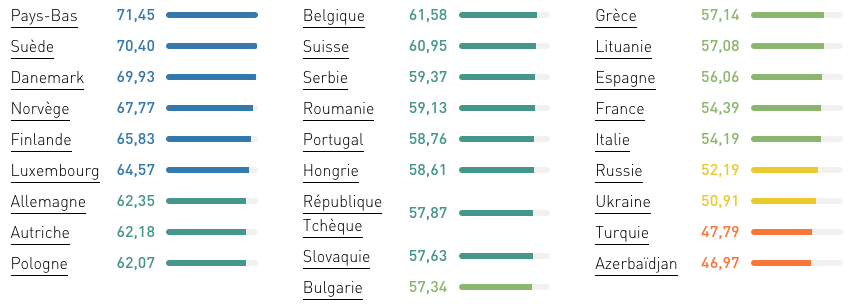
\includegraphics[scale=.5]{../img/french-english-level-in-europe}
    
    \label{fig:1}
  \end{figure}
\item niveau en anglais par rapport \href{http://doyouspeakenglish.fr/numero-1-en-tourisme-mais-dernier-en-anglais/}{au
    reste du monde}\footnote{Vous pouvez aller directement sur mon blog
  \url{http://doyouspeakenglish.fr/numero-1-en-tourisme-mais-dernier-en-anglais/} pour observer l'étude complète.}
(~derrière la République Dominicaine et la Corée du Sud s'il vous
plaît\ldots{} voir la figure \ref{fig:2} page \pageref{fig:2} pour
plus de détails~)
  \begin{figure}[h]
    \centering
    \caption[L'anglais dans le monde]{Niveau d'anglais dans le monde}\vspace{.1cm}
    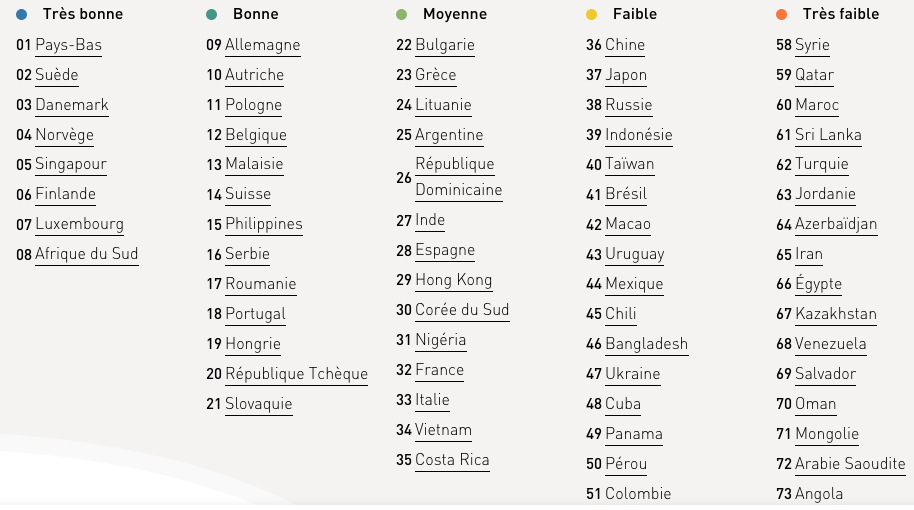
\includegraphics[scale=.5]{../img/english-level-in-the-world}
    
    \label{fig:2}
  \end{figure}
\item encore des
  \href{http://doyouspeakenglish.fr/les-francais-et-les-langues-en-quelques-chiffres/}{chiffres
    accablants}\footnote{Consulter mon article sur \url{http://doyouspeakenglish.fr/les-francais-et-les-langues-en-quelques-chiffres/}}
   
  \begin{figure}[h]
    \centering
    \caption[L'anglais en France]{Niveau d'anglais en France}\vspace{.1cm}
    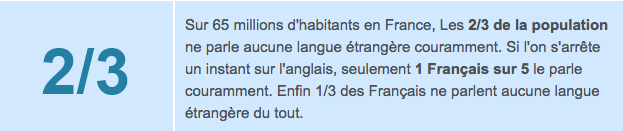
\includegraphics[scale=.725]{../img/french-english-level-in-france}
    
    \label{fig:3}
  \end{figure}
\end{itemize}
Loin de moi l'idée de vous assommer avec des chiffres et encore moins
de partir dans l'auto-flagellation. Néanmoins, il faut être lucide, il
y a un problème franco-français (~qui est très bien expliqué dans cet
\href{http://www.larevuedesressources.org/les-francais-et-les-langues-etrangeres,2920.html}{essai}~). 
Ce problème est très bien développé et analysé dans l'essai du
professeur Daniel Emilio Rojas\footnote{Lisez-le c'est gratuit, très
  bien écrit et instructif : \url{http://www.larevuedesressources.org/les-francais-et-les-langues-etrangeres,2920.html}} (~hispanophone natif qui parle et écrit
probablement beaucoup mieux le français que 90\% d'entre
nous~). Cependant, je me permettrais de vous proposer un raccourci\footnote{Forcément réducteur.} pédagogique en vous rappelant un fait
élémentaire mais que l'on oublie trop souvent. Parfois les solutions
sont tellement \underline{bêtes} qu'on oublie d'y penser. Attention, je ne
prétends pas vous proposer de recette miracle. L'anglais est une
langue difficile\footnote{Des linguistes professionnels et moi-même te
  le montrent dans cet article \url{http://doyouspeakenglish.fr/langlais-une-langue-facile/} }, bizarre, complexe et
illogique\footnote{Comme beaucoup de langues et notamment le
  français.}; et je ne suis pas le seul à le dire puisque certains anglophones natifs (~et
linguistes de surcroît~) le disent et l'écrivent par exemple dans cet \href{http://doyouspeakenglish.fr/langlais-une-langue-facile/}{article} qui permet également d'être
écouté\footnote{Comme je le montre dans cette vidéo
  \url{https://youtu.be/6wLbtx2iL7c}}. Donc oui l'anglais est
difficile, \underline{mais} avec un peu de bon sens et de persévérence
vous pouvez y arriver\footnote{Bon, il y a une triste vérité qu'il
  faut accepter, vous ne parlerez \underline{jamais} comme un natif (~\underline{sauf}
  si vous décidez de vous installer dans un pays anglophone~).}. 

\newpage
\section{Le truc tout bête}\label{sec:truc}
Mais quel est donc ce truc \underline{tout bête} que l'on oublierait et dont je
ne vous ai toujours pas parlé ? Minute papillon ! Non ! Je n'essaie
pas de noyer le poisson, je vais vous révéler mon \underline{truc}. Je vous
préviens, vous allez être probablement déçu, mais pourtant c'est une
évidence. \par
Allons-y ! Et bien, je ne sais pas pour vous mais pour moi\footnote{Et il me
semble pour la plupart des gens aussi.}, l'acquisition de ma langue
maternelle a commencé par l'oral et non par l'écrit. Pendant au moins
5 ans\footnote{Avant l'entrée au CP ou tout autre système scolaire qui
apprend à lire et à écrire.}, j'ai pratiqué en priorité l'écoute et la
méthode essai/erreur\footnote{En anglais on dit \exEN{try and guess} ce qui veut
dire \exFR{essayer et deviner}, qui est un point de vue plus positif (
attitude plus répandue chez les anglophones et en particulier chez les américains).}. Ben
oui, quand on est enfant on baigne dans un environnement linguistique
oral. Et dès les premiers mois de la vie on essaie (~avec beaucoup de
difficultés au début~) de produire ou plutôt reproduire des \textcolor{teal}{sons} que
l'on a entendu. Et croyez-moi, si vous avez oublié allez faire un tour
chez votre frère, soeur, cousin, cousine, ami, amie qui a (~ont~) des
enfants en bas âge et cela vous raffraichira la mémoire. La parole est
si importante pour l'humanité qu'elle a été pendant des siècles (~ des
millénaires même!~) le seul et unique vecteur de
communication. D'ailleurs aujourd'hui encore parmi les presque 7~000
\href{http://www.museedelhomme.fr/fr/combien-langues-sont-parlees-monde}{langues dans le monde} la plupart ne possèdent pas de système
d'écriture. Pour plus de précisions sur la répartition linguistique
dans le monde vous pouvez consulter \href{http://www.axl.cefan.ulaval.ca/Langues/1div\_recens.htm}{ce site canadien} qui tire ses
sources statistiques du \underline{Summer Institute of Linguistics} du
Texas\footnote{Voici l'url du site
  \url{http://www.axl.cefan.ulaval.ca/Langues/1div_recens.htm}}
(~2017~).\par

\newpage

\subsection{Quelques citations}\label{subsec:quote}

% \begin{bigquote}[1.0]
%   \begin{displayquote}[Extrait du livre \FL.][.]
%     Les Romains, déjà, ne parlaient pas exactement la langue qu'ils
%   écrivaient. Ainsi, \underline{cheval} vient d'un mot parlé,
%   \exLT{caballus}, alors que le latin classique écrit \exLT{equus} ---
%   d'où viendront des mots <<~savants~>> comme \underline{équidé} et
%   \underline{équitation}
%   \end{displayquote}
% \end{bigquote}  
        
\begin{center}
  \shadowbox{
    \begin{minipage}{\textwidth}
      {\fontfamily{Skia}\selectfont
        \blockquote[Extrait du livre \FL.][.]{%
          Les Romains, déjà, ne parlaient pas exactement la langue
          qu'ils écrivaient. Ainsi, \underline{cheval} vient d'un mot
          parlé, \exLT{caballus}, alors que le latin classique écrit
          \exLT{equus} --- d'où viendront des mots <<~savants~>> comme
          \underline{équidé} et \underline{équitation}%
        }
      }
    \end{minipage}%
  }
\end{center}

D'ailleurs comme le montre la première vidéo dans
\href{http://doyouspeakenglish.fr/prescriptiviste-ou-descriptiviste/}{cet
  article}, les zones du cerveau actives pour la parole et pour l'écriture sont différentes.\par

\begin{center}
  \shadowbox{
    \begin{minipage}{\textwidth}
      {\fontfamily{Skia}\selectfont
      \blockquote[Extrait du livre \FL.][.]{%
        Longtemps, le français s'est écrit comme il se parlait; vice versa,
        toutes les lettres se prononçaient, comme en latin. La notion même
        d'orthographe n'existait pas% 
      }%
      }
    \end{minipage}%
  }
\end{center}

En lisant ce dernier extrait je parie que certains d'entre vous sont en train
de chercher un moyen pour inventer une machine à remonter le temps. 

Vous vous demandez sûrement où je veux en venir. Mon but est de vous
faire comprendre ou plutôt de vous rappeler qu'une langue ça s'écoute
et ça se parle pendant un certain temps (~jusqu'à ce que ça devienne
naturel~) avant d'apprendre à l'écrire et d'étudier toutes les
subtilités de la grammaire. \href{https://fr.wikipedia.org/wiki/Django\_Reinhardt}{Django Reinhardt} et \href{https://fr.wikipedia.org/wiki/Louis\_Armstrong}{Louis Amstrong} ne
savaient ni lire ni écrire la musique et pourtant ils sont des
musiciens vénérés de leur vivant et encore aujourd'hui.\par

\newpage

\section{Une langue est une musique}\label{sec:music}
Et oui une langue c'est également une musique ! Une langue a une
musicalité et un rythme. Pas de chance pour nous le français (~ou
plutôt le \underline{parisien}\footnote{J'en parlerais plus en détails
  dans un prochain livre mais si vous êtes impatient alors je vous
  recommande de vous procurer \FL.}~)
n'est pas très chantant. Mais pourtant si l'on écoute les accents du
midi il y a tout de suite plus de mélodies qui chatouillent nos
oreilles. 

En résumé, ce que je vais partager avec vous dans ce livre, ce
sont les \textcolor{teal}{sons} de la langue anglaise. Les \href{https://pronunciationstudio.com/45-Sounds/}{45 \textcolor{teal}{sons}} (~certains en
décrivent 44, pour le français\footnote{Selon le \GE il y a 36 \textcolor{teal}{sons}
  <<~\exFR{purement}~>> français auquel on ajoute le \son~\phon{ŋ}
  hérité de l'anglais et notamment utilisé dans \exEN{parking}.} c'est
pareil, certains disent 36 d'autres 37~).\par

%\begin{itemize}
% \item Dans une première partie je vous présenterai la phonétique du
% français. En effet, il me semble plus judicieux d'approcher ce nouvel
% ensemble de symbole qui décrit les \textcolor{teal}{sons} avec précisément des \textcolor{teal}{sons} que
% vous utilisez déjà tous les jours.
Pour conclure cette introduction je rappelerai deux faits que l'on a tendance à oublier mais qu'il faut \underline{absolument garder à l'esprit} :

\begin{enumerate}
\item Le français est une langue syllabique alors que l'anglais est
  une langue accentuelle\footnote{Consulter mon \href{http://doyouspeakenglish.fr/laccent-tonique-en-anglais/}{article} de
    blog pour plus de détals.}.
\item En français il y a 36 \textcolor{teal}{sons}\footnote{Selon le
    \GE 36 mais selon Sousa auteur du livre \HTEBL il
    n'y en aurait que 32. Pour ce chiffre j'accorderai plus de crédit
    au \GE pour la bonne et simple raison qu'en tant que linguiste
    francophone il me semble plus compétant que Sousa qui est
    anglophone.} et 250 façons\footnote{Encore une fois les
    estimations diffèrent \GE n'en compte que 130 ce qui accentue
    encore plus la complexité de l'anglais.} de les écrire alors qu'en
  anglais il y a 44 \textcolor{teal}{sons} pour 1~100 façons de les écrire\footnote{Les
    chiffres concernant les façons d'écrire sont issus des
    comparaisons présentées dans le livre \HTEBL Chapter 4 Teaching
    English Language Reading and Writing page 84 Table 4.1.}.
\end{enumerate}

Par conséquent \underline{la prononciation, l'accent et le rythme} ne sont pas
superflus mais \underline{obligatoire en anglais}.\par

% Dans la deuxième partie du livre je vais vous présenter 45
% \textcolor{teal}{sons} qui sont absolument \underline{fondamentaux}
% dans la langue anglaise. En insistant particulièrement sur ceux qui
% n'apparaissent pas du tout dans la langue française.
% Et pour bien
% faire la différence il était important de commencer par la phonétique
% de la langue française que vous ne connaissez probablement pas
% encore. C'est pour cette raison qu'il est vivement recommandé de lire ce livre dans l'ordre.
%\end{itemize}

\newpage
\section{Mini conclusion de cette introduction}\label{sec:mini}
J'ai dit qu'on apprend d'abord à parler avant d'écrire, c'est vrai,
mais a priori, si vous lisez ce livre c'est que vous savez lire. Et
comme vous savez lire et bien on va en profiter pour apprendre encore
plus efficacement en utilisant
l'\href{https://fr.wikipedia.org/wiki/Alphabet_phon\%C3\%A9tique_international}{API}\CW{https://fr.wikipedia.org/wiki/Alphabet_phon\%C3\%A9tique_international}
(~Alphabet Phonétique International~). En anglais on l'écrit
IPA\CW{https://en.wikipedia.org/wiki/International_Phonetic_Alphabet}
(~International Phonetic Alphabet~).\par

Et cerise sur le gâteau, ceci
vous sera utile pour toutes les autres langues que vous souhaitez
apprendre ou que vous parlez déjà (~cela va même améliorer votre
français~). D'ailleurs, contrairement à ce que certaines personnes
pourraient penser, apprendre une autre langue, et en particulier
l'anglais, améliore votre niveau de français\footnote{En effet il existe plus de 25~000 mots anglais
  d'origine française et vous pouvez en découvrir quelques-uns grâce
  aux cartes mémoires que j'ai créé :
  \url{https://tinycards.duolingo.com/decks/6VNKUdba/english-words-with-french-origin}
et au livre plus complet \HSQMYP.}. Ce n'est pas magique,
mais c'est véridique. Alors c'est parti, allons découvrir les 45 \textcolor{teal}{sons}\footnote{Vous pouvez déjà vous entraîner grauitement grâce
  aux cartes mémoires que j'ai créé : \url{https://tiny.cards/decks/6YTEvyrN/english-phonetics}}
de la langue anglaise (~qui n'a plus grand chose à voir avec
Shakespeare de la même manière qu'on ne parle plus la langue de
Molière~).

\newpage
\minitoc



% \part{Phonétique du français}
% Ce qui m'a frappé lors de mes recherches en apprentissage des langues,
% et en particulier en ce qui concerne les ressources francophones,
% c'est que la phonétique du français n'est présentée que pour les
% étrangers. En effet, à part dans les travaux universitaires de
% chercheurs, il rare de voir des cours de langue qui commencent par
% présenter la phonétique du français avant de présenter celle de la
% langue cible, en l'occurrence ici l'anglais. C'est comme si on vous
% apprenait la grammaire anglaise sans que vous ne connaissiez votre
% propre grammaire ou pire, si on vous apprenez le vocabulaire anglais
% sans que vous ne sachiez les liaisons qu'il existe entre les deux
% vocabulaire\footnote{Hélas c'est exactement le cas, il est très rare
%   de voir des gens présenter l'immense importance du nombre de mots
%   anglais d'origine française. Je ne saurais que trop vous recommander
% mes
% \href{https://tinycards.duolingo.com/decks/6VNKUdba/english-words-with-french-origin}{cartes
%   mémoires gratuites} et ce livre
% \href{https://www.amazon.fr/gp/product/225315444X/ref=as_li_tl?ie=UTF8&camp=1642&creative=6746&creativeASIN=225315444X&linkCode=as2&tag=wwwbecomefree-21&linkId=5317e7b0e063b4d6c7c676b11420e49d}{Honni
%   soit qui mal y pense} qui en parle plus en profondeur.}.\par
% Puisque l'on est jamais mieux servi que par soi-même j'ai décidé
% d'agir ! Alors je souhaite corriger ça en commençant par vous
% présenter la phonétique de la langue que vous utilisez au
% quotidien\footnote{Au moins lorsque vous lirez ces lignes.}, le
% français\footnote{Et si vous voulez connaître son histoire je vous
%   recommande cette série de \href{https://www.youtube.com/watch?v=rHSIPt_ehvc&list=PLH2hhYn999aRfv2odG4SozTXCHbZaX_ji}{vidéo}}. Pour
% chaque son je vous proposerai trois exemples de mots qui le
% contiennent et pour chaque mot vous trouverez une phrase d'exemple
% l'illustrant en français et la traduction de cette phrase en
% anglais. En effet, le but de ce livre et de vous permettre
% d'apprivoiser la phonétique anglaise afin de découvrir ou de parfaire
% votre apprentissage de l'anglais. De façon un peu grossière ou
% simpliste je dirais que le français est fondamentalement une langue de
% l'écrit alors que l'anglais est plutôt une langue de l'oral.\par
% Bien sûr, je ne remets aucunement en cause la richesse de la
% littérature anglaise. Mon but est simplement de souligner l'extrême
% complexité de la langue anglaise parlée en comparaison avec le
% français.\par

%\chapter{Bref historique du français en 5 étapes
  clés}\label{chap:hist}

Tout d'abord il me semble important de souligner que je ne suis ni
historien, ni linguiste, ni prof de français. Par conséquent si vous
souhaitez plus d'exhaustivité sur ce sujet je vous recommande vivement
la série de vidéos présenté par le professeur au Collège de France
Claude Hagège disponible gratuitement sur
\href{https://youtu.be/fjAuHvOMXFE}{YouTube}. Je me base
essentiellement sur l'ouvrage remarquablement concis et précis
\href{https://www.amazon.fr/gp/product/2844100015/ref=as\_li\_tl?ie=UTF8\&camp=1642\&creative=6746\&creativeASIN=2844100015\&linkCode=as2\&tag=wwwbecomefree-21\&linkId=985f3a849fd44728e8480993cf2d5490}{français
  lycée} écrit par
\href{https://fr.wikipedia.org/wiki/Pierre_Brunel#Autres}{Pierre
  Brunel}.

\begin{quote}
  \'Elève à l'\'Ecole normale supérieure (1958), il est
  reçu premier à l'agrégation de lettres classiques en 1962, puis
  prépare deux thèses sur Paul Claudel, obtenant son doctorat d'\'Etat
  en 1970.
\end{quote}

Voilà pour une brève présentation de Monsieur Brunel qui fera office
de source principale pour ce que je présenterai dans ce chapitre. Si
vous souhaitez absolument un ouvrage de référence sur le sujet alors
je ne saurais que trop vous recommander l'ouvrage complet, rigoureux
et sérieux du linguiste français Alain Rey\footnote{Attention, il
  s'agit d'un ouvrage conséquent 672 pages rien que pour le tome1 et
  donc il y a aussi un tome~2 !} \href{https://www.amazon.fr/gp/product/2262033110/ref=as_li_tl?ie=UTF8&camp=1642&creative=6746&creativeASIN=2262033110&linkCode=as2&tag=wwwbecomefree-21&linkId=2be27c37e2162a822bb18af72db66042}{Mille ans de langue
  française tome 1}.\par

Et si vous vous intéressez en particulier à l'histoire de France alors
je vous recommande l'excellent ouvrage de Jean-Paul
Demoule\footnote{Vous pouvez déjà consulter son intervention dans
  une émission de Mediapart disponible sur \href{https://youtu.be/IMpHyq2gq7g?t=15m18s}{YouTube}.} \href{https://www.amazon.fr/gp/product/B00GNJHMUI/ref=as_li_tl?ie=UTF8&camp=1642&creative=6746&creativeASIN=B00GNJHMUI&linkCode=as2&tag=wwwbecomefree-21&linkId=d4b515d26f9ade9ea3e0759b397590a2}{On
  a retrouvé l'histoire de France}.\par

Bon après toutes ces recommandations de lectures textuelles ou
visuelles, passons à présent au vif du sujet.\par

Alors voici le plan en 5 étapes :

\begin{enumerate}
\item Les origines de la langue française
\item Du français au latin
\item L'unification de la langue
\item La fixation de l'orthographe
\item La fixation de la grammaire
\end{enumerate}

Bien entendu, si vous êtes fâché avec l'histoire, ou si vous voulez
uniquement acquérir une compétence technique, ou si vous n'avez pas le
temps vous pouvez directement passer au chapitre n\no~\ref{chap:voy} page~\pageref{chap:voy}. En revanche,
dans tous les cas je vous recommande d'étudier la phonétique française
\underline{avant} celle de l'anglais.

\newpage
\minitoc
\newpage
\section{Les origines de la langue française}\label{sec:orgfr}

\begin{quote}
  Le français est au croisement du latin et du germain, l'ancien
  allemand. Le fond celte -- gaulois -- est presque totalement oublié,
  sauf dans quelques noms de lieux.
\end{quote}

Dès le départ le ton est donné dans l'ouvrage de Pierre
Brunel\footnote{Il s'agit de l'introduction  de la partie du livre \href{https://www.amazon.fr/gp/product/2844100015/ref=as\_li\_tl?ie=UTF8\&camp=1642\&creative=6746\&creativeASIN=2844100015\&linkCode=as2\&tag=wwwbecomefree-21\&linkId=985f3a849fd44728e8480993cf2d5490}{français
  lycée} consacrée aux origines de la langue française.}. Bon, comme
annoncé plus haut, je ne suis ni historien, ni linguiste, ni prof de
français par conséquent je vais aller droit au but.\par

\subsection{Le fond latin}\label{subsec:lat}

Entre 58 et 52 avant notre ère la Gaule est conquise par les
Romains. Conséquence immédiate, le peuple de Gaule\footnote{Comme la
  plupart des autres régions dominées par l'empire romain\dots à part
  d'irréductible <<~grands-bretons~>> et autres écossais\dots mais
  c'est une autre histoire dont nous parlerons dans un prochain
  chapitre.} se met à parler le latin (par forcément par gaieté de
c{\oe}ur nous en conviendrons).\par

Laissez mijoter pendant deux siècles environ et voilà pourquoi lorsque
les barbares arrivent\dots ben les Gaulois parlent vraiment latin.

\subsection{Le fond germanique}\label{subsec:germ}

Les invasions germaniques au moment de la chute de Rome, en 410, sont
à l'origine d'une nouvelle transformation linguistique. Mais cette
fois-ci c'est l'envahisseur qui va adopter la langue locale et non
imposer la sienne. D'ailleurs il me semble avoir appris à l'école que
le commencement de la France serait le baptême de Clovis, rois des
Francs originaires de Saxe\footnote{Comment appelle-t-on les habitants
de la Saxe déjà ? Les Saxons ! C'est marrant c'est comme dans
anglo-saxon\dots élémentaire mon cher Watson !} en 496.\par
En résumé, après avoir été latinisés, les gaulois ont été germanisés
mais ont gardé le latin et la chrétienté comme héritage culturel
dominant.

\section{Du latin au français}\label{sec:lat2fr}

\begin{quote}
  Les Romains ont envahi la Gaule par le sud : les langues d'oc sont
  donc plus proches du latin que les langues d'oïl.
\end{quote}

La citation du livre de Pierre Brunel\footnote{Comme annoncé plus haut
je me base toujours sur le livre \href{https://www.amazon.fr/gp/product/2844100015/ref=as\_li\_tl?ie=UTF8\&camp=1642\&creative=6746\&creativeASIN=2844100015\&linkCode=as2\&tag=wwwbecomefree-21\&linkId=985f3a849fd44728e8480993cf2d5490}{français
  lycée} que je recommande chaleureusement pour plus de détails.} a le
mérite d'être claire, concise et limpide.

\subsection{Langue d'oc, langue d'oïl}\label{subsec:langOcOil}

\begin{quotation}
  Oc et oil sont les deux manières de dire oui, au sud et au nord de
  la Loire, qui figure la barrière symbolique entre les deux parties
  du territoire.\par
  Plus proches de la langue cultivée qu'est le latin, les langues d'oc
  -- qui donneront son nom à la région Languedoc -- correspondent
  également à une civilisation moins brutale que celle du Nord. [\dots]
\end{quotation}

Je précise que l'auteur n'a pas mis le tréma mais sur
\href{https://fr.wikipedia.org/wiki/Langue_d\%27o\%C3\%AFl}{Wikipédia}\footnote{Qui propose en plus la phonétique ce qui m'incite à
  leur faire plus confiance sur ce point particulier (prononciation :
  o-il [ɔ.il], ou-il [u.il], oui [wi], o-ille [ɔj]).}


\begin{subfigures}
  \label{fig:fig4a5}
  %
  \begin{figure}
    \centering
    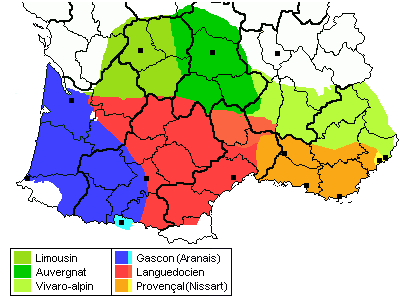
\includegraphics[scale=.725]{../img/langOc.png}
    \caption{Langue d'Oc}
    \label{fig:fig4}
  \end{figure}
  %
  \begin{figure}
    \centering
    \includegraphics[scale=.0725]{../img/langOil.png}
    \caption{Langue d'Oïl}
    \label{fig:fig5}
  \end{figure}
  %
\end{subfigures}

\subsection{L'ancien français}\label{subsec:ancienfr}

\begin{quotation}
  C'est la langue parlée au nord de la Loire. Du latin, elle garde
  l'essentiel de son vocabulaire, transformé par les prononciations
  locales, ainsi qu'une petite partie de sa grammaire, simplifiée :
  l'ancien français a encore une déclinaison, mais à deux cas
  seulement -- sujet et régime -- là ou le latin en comptait
  six. L'ordre des mots usuel\footnote{Vous trouverez facilement sur
    internet ou dans des ouvrages l'abréviation SVO pour \exFR{Sujet Verbe
    Objet} (\exEN{Subject Verb Object}).} -- sujet / verbe / complément -- est
  inédit : le latin s'exprimait dans l'ordre sujet / complément / verbe.
\end{quotation}

Pierre Brunel a tout dit dans cette sous-section alors passons à la
suite.

\subsection{Langue savante, langue vivante}\label{subsec:lslv}

\begin{quotation}
  Le latin populaire évolue très vite parce qu'il est parlé, souvent
  mal\footnote{Exactement comme l'anglais aujourd'hui.}, dans tout
  l'Empire. Il est à l'origine de l'ensemble des langues romanes que
  nous connaissons aujourd'hui -- italien, espagnol, portugais,
  roumain -- ainsi que de l'essentiel du français.
  La tradition du latin écrit est perpétuée par les moines. Elle fixe
  rapidement une langue de culture opposée aux langues populaires qui
  ne s'écrivent que très tardivement.
\end{quotation}

Durant le Moyen Âge 80\% de la littérature européenne est écrite en
latin, véritable lingua franca des élites intellectuelles. C'est aussi
la langue des sciences (et ça le restera encore
longtemps\footnote{Pensez à Newton qui a écrit son ouvrage majeur
  Principia Mathematica en latin.}). C'est d'ailleurs l'\'Eglise qui
contrôle les universités en Europe.


\section{L'unification de la langue}\label{sec:unifr}

\begin{quote}
  Le français s'est imposé très lentement, non seulement dans l'usage
  littéraire, dominé par le latin, mais dans la vie de tous les jours,
  où règnaient les langues régionales.
\end{quote}

\subsection{Un royaume éclaté en provinces}\label{subsec:roysplit}

\begin{quotation}
  Le sud de la France qui n'est pas, au Moyen Âge, encore intégré au
  royaume, est déjà framenté en divers <<~pays~>> dont les langues,
  pour proches qu'elles soient, ne sont pas absolument semblables.
  Ainsi, l4auvergne parle une langue d'oc que comprennent mal les gens
  de Bordeaux ou de Toulon.
  Au nord, la situation se complique. Seuls l'Île-de-France,
  l'Orléanais, la Picardie, la Normandie et l'Artois parlent français,
  avec des variantes.
  La Bourgogne -- du nord de Lyon aux Ardennes et de la Champagne à
  l'Alsace -- est pour l'essentiel un territoire germanique.
  La Bretagne est le refuge des derniers Celtes.
  Aux langues se superposent, de plus, des <<~patois~>>, utilisés sur
  des aires géographique plus restreintes, qui sont pafois peu compréhensibles.
\end{quotation}

\subsection{Le triomphe du Nord}\label{subsec:trinord}

\begin{quote}
  La plus grande unité politique de la France du Nord, la volonté
  expansionniste des rois de France, le fait que le Sud soit dans
  l'aire d'expansion arabe -- ce qui l'enrichit mais aussi le menace
  -- tout se ligue pour imposer la langue d'oil.
  Mais il faut attendre le \textsc{\romannumeral 15}\up{e}~siècle pour
  que la domination politique devienne une domination culturelle.
\end{quote}

\subsection{La langue du roi}\label{subsec:langroy}
\begin{quotation}
  L'édit de Villers-Cotterêts\footnote{Certaines personnes remettent
    en cause son importance comme dans cette \href{https://youtu.be/x3TQkQO_XMc}{vidéo}}, promulgué par François
  {\scshape{\romannumeral 1}}\up{er} en 1539, impose l'usage de la langue
  française dans les tribunaux. Ceux-ci utilisaient jusqu'alors
  exclusivement le latin et leurs décisions étaient donc mal comprises
  par le peuple.
  L'installation définitive de la cour du roi en Île-de-France impose
  peu à peu l'usage de la langue française aux seigneurs qui entourent
  le souverain.
\end{quotation}

\section{La fixation de l'orthographe}\label{sec:orthofix}

\begin{quote}
  Longtemps, le français s'est écrit comme il se parlait; vice versa,
  toutes les lettres se prononçaient, comme en latin. La notion même
  d'orthographe n'existait pas.
\end{quote}

\subsection{L'anarchie médiévale}\label{subsec:arnar}

\begin{quotation}
  Au Moyen Âge, il y a autant d'orthographes que de scripteurs. Les
  scribes, surtout des moines, sont plus intéressés par l'esthétique
  de leurs manuscrits que par une <<~correction~>> dont l'idée même
  n'existe pas. Ils ajoutent parfois des lettres, transforment un i en
  y pour bénéficier d'une courbe élégante.
  Les aristocrates, qui peu à peu apprennent à écrire, se soucient peu
  d'orthographe. 
\end{quotation}

\subsection{Les réformateurs du \textsc{\romannumeral
    16}\up{e}~siècle}\label{subsec:ref}
\begin{quotation}
  Plusieurs grammairiens comme Robert Estienne veulent écrire le
  français comme on l'entend et proposent des réformes visant à
  simplifier la graphie.
  On invente les accents pour rendre compte de la prononciation. On
  tente de supprimer les lettres qui ne se prononcent pas -- par
  exemple certains s terminaux hérités de la déclinaison de l'ancien
  français et la plupart des lettres doubles.
  L'absence de dictionnaire et, surtout, le manque d'intérêt des
  dirigeants, rendent toute généralisation difficile, d'autant que
  certains réformateurs, des humanistes tentés par la Réforme,
  manquent d'appuis à la Cour.
\end{quotation}

\subsection{Le triomphe des latinisants}\label{subsec:trilat}

\begin{quotation}
  Du Bellay affirme que le français vaut bien le latin : toutefois,
  langue et culture latines restent exemplaires. On justifie donc
  l'orthographe par l'étymologie et on invente des séries de mots sur
  leur modèle latin. Ainsi, à partir de confidentia, qui avait évolué
  en confiance, on fabrique confidence.
\end{quotation}

\section{La fixation de la grammaire}\label{sec:fixgram}

\begin{quote}
  Largement tributaire du latin pour son vocabulaire, le français s'en
  dégage radicalement dans sa grammaire. Mais il n'a imposé ses
  différences que peu à peu.
\end{quote}

\subsection{La fin des déclinaisons}\label{subsec:findec}

\begin{quotation}
  Entre l'ancien français (\textsc{\romannumeral 9}\up{e} -
\textsc{\romannumeral 16}\up{e}~siècle) et le français moderne (à
partir du \textsc{\romannumeral 16}\up{e}~siècle), on distingue
souvent une période intermédiaire de <<~moyen français~>>
(\textsc{\romannumeral 15}\up{e}~siècle) durant laquelle se fixent les
caractères de la langue moderne -- en particulier, la disparition de
la déclinaison. L'ancien français avait deux cas, afin de distinguer
les sujets et les autres fonctions.
Dorénavant, seules subsistent les distinctions entre singulier et pluriel.
\end{quotation}

\subsection{L'ordre des mots de la phrase}\label{subsec:ordmot}

\begin{quotation}
  Le latin, surtout en poésie, pouvait se permettre un ordre des mots
  fantaisiste, puisque les déclinaisons indiquaient la fonction
  grammaticale. Il en est de même, de façon très atténuée, en ancien
  français. C'est la disparition des déclinaisons qui impose l'ordre
  régulier de la phrase de base -- sujet / verbe / complément --, que
  seuls les poètes oseront encore enfreindre. De même, la disparition
  de finales discriminantes impose l'usage généralisé de l'article,
  que le latin ignorait et que l'ancien français pratiquait modérément.
\end{quotation}

\subsection{Une langue épurée}\label{langpur}

\begin{quotation}
  Les poètes de la Pléiade manifestaient une grande liberté
  d'invention lexicale.
  Mais, dès le début du \textsc{\romannumeral 17}\up{e}~siècle,
  Malherbe reprend en main la grammaire et le lexique en fixant des
  bornes très étroites à l'innovation.
  Les mots d'origine provinciales sont bannis pour <<~gasconnisme~>>
  -- du nom de la province de Gascogne. On crée le terme éloquent de
  <<~barbarisme~>> -- <<~propre à la façon de parler des barbares~>>
  -- pour désigner tout mot peu conforme au <<~génie de la
  langue~>>. L'axe Rouen-Paris domine la vie intellectuelle de façon
  autoritaire. On épure la langue au nom du roi\dots pour mieux
  l'imposer au roi -- Henri \textsc{\romannumeral 4} est Gascon --
  ainsi qu'à son entourage, souvent composés d'<<~étrangers~>>. On
  interdira bientôt l'usage de tel ou tel terme décrété
  <<~mal-sonnant~>> ou <<~bas~>>. La langue littéraire ne vivra
  désormais plus que dans une atmosphère raréfiée.
\end{quotation}

\newpage
\minitoc


%\chapter{Voyelles}\label{chap:voy}
Que celui ou celle qui a dit <<~consonne~>> juste après avoir lu le
titre du chapitre sorte immédiatement\footnote{Toute référence à une
  émission de la télévision française serait purement fortuite, un
  coup du hasard si j'ose pousser légèrement la prose.}!\par
Plus sérieusement, lorsqu'on regroupe les voyelles\footnote{Puisque ce
  livre parle de phonétique on s'occupe des sons donc de l'oral et pas
  de l'écrit (donc on se fiche qu'il y ait six voyelles écrites).} on
découvre deux grandes catégories : les voyelles dites \exFR{Orales} et
les voyelles dites \exFR{Nasales}\footnote{Que les anglophones ont du
  mal à prononcer correcement.}.

Un son de voyelle est fait en façonnant l'air comme il quitte la
bouche. Nous utilisons les articulateurs pour façonner l'air - les
lèvres, la mâchoire, la langue. La langue française parlée compte
ainsi seize voyelles, 12 orales et 4 nasales.

\section{Voyelles orales}\label{sec:orales}
\subsection{Le son [a]}\label{subsec:afr}

C'est le son que l'on trouve dans les mots \exFR{arrêt} (/aʀɛ/),
\exFR{bar} (/baʀ/), \exFR{chat} (/ʃa/), et bien
d'autres. 

Observons un exemple pour chacun d'entre eux et voyons leurs
traductions anglaises :\par

\begin{enumerate}
\item \exFR{arrêt} (/aʀɛ/)
  \begin{itemize}
  \item \exFR{Ce matin j'ai attendu à l'arrêt de
      bus pendant dix  minutes.}
    \item \exEN{This morning I waited at the bus stop for ten minutes.}
    \end{itemize}
    Le mot \exEN{stop} est même utilisé dans la langue française
    au point que certaines personnes le conjuguent (\textquote[][.]{\exFR{J'ai stoppé net quand j'ai vu la voiture arriver}}).
    Cependant en anglais on
    prononce
    \href{https://en.oxforddictionaries.com/definition/stop}{/stɒp/}
    alors qu'en français on le prononce
    \href{http://www.wordreference.com/fren/stop}{/stɔp/}\footnote{Les
      sons [ɒ] et [ɔ] sont bien distincts}.
\item \exFR{bar} (/baʀ/)
  \begin{itemize}
  \item \exFR{Dans la rue où j'ai grandi il y
      avait un bar juste en bas de chez moi.}
  \item \exEN{In the street where I grew up there was a bar just down from my house.}
  \end{itemize}
    Attention ! Les deux mots sont homographes\footnote{Deux mots sont
      dits homographes s'ils s'écrivent de la même manière (avec les
      mêmes lettres).} mais ils ne sont pas homophones\footnote{Deux
      mots sont dits homophones s'ils se prononcent de la même façon
      (même son).} ! En effet, en anglais on prononce
    \href{https://en.oxforddictionaries.com/definition/bar}{/bɑː/}
    alors qu'en français on dit \href{http://www.wordreference.com/fren/bar}{/baʀ/}; voilà un exemple qui illustre parfaitement l'intérêt
    d'étudier la phonétique.
  \item \exFR{chat} (/ʃa/)
    \begin{itemize}
    \item \exFR{Le chat des voisins vient souvent nous rendre visite.}
    \item \exEN{The neighbor's cat often comes to visit us.}
    \end{itemize}
    Ici on a d'une part \exFR{chat} qui se prononce
    \href{http://www.wordreference.com/fren/chat}{/ʃa/} en français et
    \exEN{cat} en anglais qui se prononce
    \href{http://www.wordreference.com/enfr/cat}{/kæt/}. Attention !
    Le verbe anglais \exEN{to chat}\footnote{\exEN{To chat} signifie
      bavarder.} se prononce
    \href{https://en.oxforddictionaries.com/definition/chat}{/tʃæt/}. 
\end{enumerate}

\subsection{Le son [ɑ]}\label{subsec:ɑfr}

C'est le son que l'on trouve dans les mots \exFR{bâton} (/bɑtɔ̃ /),
\exFR{mât} (/mɑ/), \exFR{pâte} (/pɑt/), et bien d'autres.

Observons un exemple pour chacun d'entre eux et voyons leurs
traductions anglaises :\par

\begin{enumerate}
\item \exFR{bâton} (/bɑtɔ̃ /)
  \begin{itemize}
  \item \exFR{Souvent dans la liste des fournitures scolaires on demande
      un bâton de colle.}
    \item \exEN{Often in the list of school supplies we ask for a stick of glue.}
    \end{itemize}
    Le mot \exEN{stick}\footnote{Le mot \exEN{stick} signifie \exFR{bâton} et
      peut aussi vouloir dire \exFR{matraque}.} se prononce en anglais \href{https://en.oxforddictionaries.com/definition/stick}{/stɪk/}.
\item \exFR{mât} (/mɑ/)
  \begin{itemize}
  \item \exFR{Avant l'invention du moteur les bateaux étaient tous à
      voile et par conséquent il fallait bien que quelqu'un grimpe au
      sommet du mât pour l'accrocher.}
  \item \exEN{Before the invention of the engine the boats were all sailing and therefore it was necessary that someone climbs to the top of the mast to hang it.}
  \end{itemize}
  En anglais le mot \exEN{mast} se prononce
  \href{https://en.oxforddictionaries.com/definition/mast}{/mɑːst/}. En
  quelques sortes on peut dire qu'il est une prolongation sonore de son
  équivalent français.

  \item \exFR{pâte} (/pɑt/)
    \begin{itemize}
    \item \exFR{Pour faire des crêpes il faut d'abord préparer la pâte.}
    \item \exEN{To make pancakes it is necessary to first prepare the dough.}
    \end{itemize}
    On notera que le mot français \exFR{pâte}\footnote{Vous pouvez consulter
      directement les traductions disponibles sur \url{http://www.wordreference.com/fren/p\%C3\%A2te}} admet de nombreux
    équivalents anglais \exEN{pastry} (pour les tartes ou
    pâtisseries), \exEN{dough} (pour le pain et les crêpes),
    \exEN{base} (pour les pizzas) et j'en passe et des meilleurs ! 
\end{enumerate}

\subsection{Le son [e]}\label{subsec:efr}

C'est un son que l'on trouve par exemple dans les mots \exFR{créer}
(/kʀee/), \exFR{pré} (/pʀe/), \exFR{république} (/ʀepyblik/), et bien d'autres.

Observons un exemple pour chacun d'entre eux et voyons leurs
traductions anglaises :\par

\begin{enumerate}
\item \exFR{créer} (/kʀee/)
  \begin{itemize}
  \item \exFR{Créer est un acte souvent solitaire mais qui s'appuie
      également sur les travaux des autres.}
    \item \exEN{Creating is often a lonely act, but it is also based on the work of others.}
    \end{itemize}
    Le verbe anglais \exEN{create} se prononce
    \href{https://en.oxforddictionaries.com/definition/create}{/kriːˈeɪt/}.
\item \exFR{pré} (/pʀe/)
  \begin{itemize}
  \item \exFR{Dans le pré il y a les vaches qui broutent de l'herbe.}
  \item \exEN{In the meadow there are cows grazing grass.}
  \end{itemize}
  

\item \exFR{république} (/ʀepyblik/)
  \begin{itemize}
  \item \exFR{La France est une république.}
  \item \exEN{France is a republic.}
  \end{itemize}
  Même si les deux mots se ressemblent beaucoup graphiquement, ils
  ne se prononcent pas de la même manière. En effet, le mot
  \exEN{republic} se prononce \href{https://en.oxforddictionaries.com/definition/republic}{/rɪˈpʌblɪk/}. 
\end{enumerate}

  
\subsection{Le son [ɛ]}\label{subsec:ɛfr}

C'est un son que l'on trouve par exemple dans les mots \exFR{carrière}
(/kaʀjɛʀ/), \exFR{mère} (/mɛʀ/), \exFR{taire} (/tɛʀ/), et bien d'autres.

Observons un exemple pour chacun d'entre eux et voyons leurs
traductions anglaises :\par

\begin{enumerate}
\item \exFR{carrière} (/kaʀjɛʀ/)
  \begin{itemize}
  \item \exFR{Généralement les sportifs de haut niveau finissent leur
      carrière avant 40 ans.}
    \item \exEN{Generally top athletes finish their career before 40 years.}
    \end{itemize}
    Le mot français \exFR{carrière} est polysémique\footnote{Il a
      plusieurs significations différentes.} mais en anglais chaque
    sens du mot français\footnote{Vous pouvez en consulter une liste
      ici \url{http://www.wordreference.com/fren/carri\%C3\%A8re}.}  correspond à un mot différent. Par exemple
    \exEN{quarry}
    (\href{https://en.oxforddictionaries.com/definition/quarry}{
      /ˈkwɒrɪ/}) pour les carrières de pierres ou encore \exEN{career}
    (\href{https://en.oxforddictionaries.com/definition/career}{/kəˈrɪə/})
    pour la carrière professionnelle.
\item \exFR{mère} (/mɛʀ/)
  \begin{itemize}
  \item \exFR{C'est à toutes les mères que je dédicace ce livre.}
  \item \exEN{It is to all the mothers that I dedicate this book.}
  \end{itemize}

  
\item \exFR{taire} (/tɛʀ/)
  \begin{itemize}
  \item \exFR{Parfois pour plaire il vaut mieux se taire.}
  \item \exEN{Sometimes to please it is better to be quiet.}
  \end{itemize}
   
\end{enumerate}

\subsection{Le son [ə]}\label{subsec:əfr}

C'est un son que l'on trouve par exemple dans les mots
\exFR{appartement} (/apaʀtəmɑ̃ /), \exFR{chemin} (/ʃ(ə)mɛ̃ /), \exFR{venin} (/vənɛ̃ /), et bien d'autres.

Observons un exemple pour chacun d'entre eux et voyons leurs
traductions anglaises :\par

\begin{enumerate}
\item \exFR{appartement} (/apaʀtəmɑ̃ /)
  \begin{itemize}
  \item \exFR{En ce moment je loue un appartement.}
    \item \exEN{At the moment I am renting an apartment.}
    \end{itemize}
    
\item \exFR{chemin} (/ʃ(ə)mɛ̃ /)
  \begin{itemize}
  \item \exFR{Le chemin de gauche permet de mieux voir la nature.}
  \item \exEN{The path on the left makes it easier to see nature.}
  \end{itemize}

  
\item \exFR{venin} (/vənɛ̃ /)
  \begin{itemize}
  \item \exFR{Gare aux serpents qui ont du venin.}
  \item \exEN{Beware of snakes with venom.}
  \end{itemize}
   
\end{enumerate}

\subsection{Le son [i]}\label{subsec:ifr}

C'est un son que l'on trouve par exemple dans les mots
\exFR{cri} (/kʀi/), \exFR{ravi} (/ʀavi/), \exFR{tri} (/tʀi/), et bien d'autres.

Observons un exemple pour chacun d'entre eux et voyons leurs
traductions anglaises :\par

\begin{enumerate}
\item \exFR{cri} (/kʀi/)
  \begin{itemize}
  \item \exFR{Je marchais seul dans la rue quand soudain j'entendis un
      cri !}
    \item \exEN{I walked alone in the street when suddenly I heard a scream!}
    \end{itemize}
    
\item \exFR{ravi} (/ʀavi/)
  \begin{itemize}
  \item \exFR{Je suis ravi de faire votre connaissance.}
  \item \exEN{I'm delighted to meet you.}
  \end{itemize}

  
\item \exFR{tri} (/tʀi/)
  \begin{itemize}
  \item \exFR{De temps en temps il est bon de faire du tri dans les
      fichiers et dossiers de l'ordinateur.}
  \item \exEN{From time to time it is good to sort through the files
      and folders of the computer.}
  \end{itemize}
   
\end{enumerate}

\subsection{Le son [o]}\label{subsec:ofr}

C'est un son que l'on trouve par exemple dans les mots
 \exFR{arroser} (/aʀoze/), \exFR{prose} (/pʀoz/), \exFR{rose} (/ʀoz/), et bien d'autres.

Observons un exemple pour chacun d'entre eux et voyons leurs
traductions anglaises :\par

\begin{enumerate}
\item  \exFR{arroser} (/aʀoze/)
  \begin{itemize}
  \item \exFR{N'oublie pas d'arroser les plantes.}
    \item \exEN{Do not forget to water the plants.}
    \end{itemize}
    
\item \exFR{prose} (/pʀoz/)
  \begin{itemize}
  \item \exFR{La prose est un style littéraire.}
  \item \exEN{Prose is a literary style.}
  \end{itemize}

  
\item \exFR{rose} (/ʀoz/)
  \begin{itemize}
  \item \exFR{À Paris, aux terrasses de café, il y a souvent des vendeurs de roses qui viennent vous demander d'en acheter.}
  \item \exEN{In Paris, on the terraces of coffee, there are often vendors of roses who come to ask you to buy some.}
  \end{itemize}
   
\end{enumerate}


\subsection{Le son [ɔ]}\label{subsec:ɔfr}

C'est un son que l'on trouve par exemple dans les mots
\exFR{cote} (/kɔt/), \exFR{note} (/nɔt/), \exFR{vote} (/vɔt/), et bien d'autres.

Observons un exemple pour chacun d'entre eux et voyons leurs
traductions anglaises :\par

\begin{enumerate}
\item  \exFR{cote} (/kɔt/)
  \begin{itemize}
  \item \exFR{Le président n'a plus la même cote de popularité qu'auparavant.}
    \item \exEN{The president no longer has the same popularity rating as before.}
    \end{itemize}
    
\item \exFR{note} (/nɔt/)
  \begin{itemize}
  \item \exFR{La question de la note est souvent un sujet qui fâche.}
  \item \exEN{The question of the note is often an annoying subject.}
  \end{itemize}

\item \exFR{vote} (/vɔt/)
  \begin{itemize}
  \item \exFR{Une chose est sûre, le résultat du vote ne fera pas que
      des heureux.}
  \item \exEN{One thing is certain, the result of the vote will not only make people happy.}
  \end{itemize}
   
\end{enumerate}
         
\subsection{Le son [ø]}\label{subsec:øfr}

C'est un son que l'on trouve par exemple dans les mots
\exFR{cieux} (/sjø/), \exFR{lieu} (/ljø/), \exFR{pieu} (/pjø/), et bien d'autres.

Observons un exemple pour chacun d'entre eux et voyons leurs
traductions anglaises :\par

\begin{enumerate}
\item  \exFR{cieux} (/sjø/)
  \begin{itemize}
  \item \exFR{Les anciens regardaient vers les cieux dans l'espoir d'y
    trouver des réponses à leurs questionnements.}
    \item \exEN{The elders looked to the heavens in the hope of finding answers to their questions.}
    \end{itemize}
    
\item \exFR{lieu} (/ljø/)
  \begin{itemize}
  \item \exFR{Voici notre lieu de rendez-vous.}
  \item \exEN{Here is our meeting place.}
  \end{itemize}

\item \exFR{pieu} (/pjø/)
  \begin{itemize}
  \item \exFR{Dans les films de vampires on préconise de leur planter
      un pieu dans le c{\oe}ur pour s'en débarrasser.}
  \item \exEN{In vampire movies it is recommended to plant a stake in the heart to get rid of it.}
  \end{itemize}
   
\end{enumerate}         

\subsection{Le son [œ]}\label{subsec:œfr}

C'est un son que l'on trouve par exemple dans les mots
\exFR{frayeur} (/fʀɛjœʀ/), \exFR{peur} (/pœʀ/), \exFR{tailleur} (/tɑjœʀ/), et bien d'autres.

Observons un exemple pour chacun d'entre eux et voyons leurs
traductions anglaises :\par

\begin{enumerate}
\item \exFR{frayeur} (/fʀɛjœʀ/)
  \begin{itemize}
  \item \exFR{Tu m'as fait une frayeur toute à l'heure quand tu as
      traversé la route sans regarder.}
    \item \exEN{You scared me earlier when you crossed the road without looking.}
    \end{itemize}
    
\item \exFR{peur} (/pœʀ/)
  \begin{itemize}
  \item \exFR{Est-ce que tu aimes avoir peur au cinéma ?}
  \item \exEN{Do you like to be afraid in the cinema?}
  \end{itemize}

\item \exFR{tailleur} (/tɑjœʀ/)
  \begin{itemize}
  \item \exFR{Pour méditer il est recommandé de s'asseoir en tailleur.}
  \item \exEN{To meditate it is recommended to sit cross-legged.}
  \end{itemize}
   
\end{enumerate}         
        
\subsection{Le son [u]}\label{subsec:ufr}

C'est un son que l'on trouve par exemple dans les mots
\exFR{nous} (/nu/), \exFR{sous} /su/, \exFR{tous} (/tus/), et bien d'autres.

Observons un exemple pour chacun d'entre eux et voyons leurs
traductions anglaises :\par

\begin{enumerate}
\item \exFR{nous} (/nu/)
  \begin{itemize}
  \item \exFR{Nous avons plutôt bien avancé, je suis fier de vous.}
    \item \exEN{We have made quite good progress, I am proud of you.}
    \end{itemize}
    
\item \exFR{sous} /su/
  \begin{itemize}
  \item \exFR{Sous le soleil exactement.}
  \item \exEN{Exactly under the sun.}
  \end{itemize}

\item \exFR{tous} (/tus/)
  \begin{itemize}
  \item \exFR{Un pour tous et tous pour un.}
  \item \exEN{One for all and all for one.}
  \end{itemize}
   
\end{enumerate}         
        
\subsection{Le son [y]}\label{subsec:yfr}

C'est un son que l'on trouve par exemple dans les mots
\exFR{fur} (/fyʀ/), \exFR{pur} (/pyʀ/), \exFR{saturer} (/satyʀe/), et bien d'autres.

Observons un exemple pour chacun d'entre eux et voyons leurs
traductions anglaises :\par

\begin{enumerate}
\item \exFR{fur} (/fyʀ/)
  \begin{itemize}
  \item \exFR{Au fur et à mesure de la pratique l'expérience
      s'acquiert patiemment.}
    \item \exEN{As the practice progresses, experience is patiently acquired.}
    \end{itemize}
\item \exFR{pur} (/pyʀ/)
  \begin{itemize}
  \item \exFR{Paradoxalement, un son pur\footnote{Je ne peux que vous
        recommander le livre \href{https://www.amazon.fr/gp/product/2841691527/ref=as_li_tl?ie=UTF8&camp=1642&creative=6746&creativeASIN=2841691527&linkCode=as2&tag=wwwbecomefree-21&linkId=bae3b8d9f1cf846547085459e99db652}{Histoire de l'acoustique
          musicale} qui explique très bien cela, bien mieux que je ne
        saurais le faire ici.} est très désagréable à l'oreille.}
  \item \exEN{Paradoxically, a pure sound is very unpleasant to the ear.}
  \end{itemize}

\item \exFR{saturer} (/satyʀe/)
  \begin{itemize}
  \item \exFR{C'est Jimi Hendrix qui a lancé la mode qui consiste à
      saturer le son de sa guitare électrique.}
  \item \exEN{Jimi Hendrix launched the fashion of saturating the sound of his electric guitar.}
  \end{itemize}
   
\end{enumerate}         


\section{Voyelles nasales}\label{sec:nasales}
\subsection{Le son [ɑ̃]}\label{subsec:atfr}
C'est un son que l'on trouve par exemple dans les mots
\exFR{arranger} (/aʀɑ̃ ʒe/), \exFR{frange} (/fʀɑ̃ ʒ/), \exFR{manger} (/mɑ̃ ʒe/), et bien d'autres.

Observons un exemple pour chacun d'entre eux et voyons leurs
traductions anglaises :\par

\begin{enumerate}
\item \exFR{arranger} (/aʀɑ̃ ʒe/)
  \begin{itemize}
  \item \exFR{J'espère que les choses vont s'arranger pour vous.}
    \item \exEN{I hope things will work out for you.}
    \end{itemize}
\item \exFR{frange} (/fʀɑ̃ ʒ/)
  \begin{itemize}
  \item \exFR{Il y a des femmes pour lesquelles la frange est un bon choix.}
  \item \exEN{There are women for whom bangs are a good choice.}
  \end{itemize}
\item \exFR{manger} (/mɑ̃ ʒe/)
  \begin{itemize}
  \item \exFR{Il faut manger pour vivre et non vivre pour manger.}
  \item \exEN{You have to eat to live and not live to eat.}
  \end{itemize}
\end{enumerate}         

\subsection{Le son [ɛ̃]}\label{subsec:etfr}
C'est un son que l'on trouve par exemple dans les mots
\exFR{larcin} (/laʀsɛ̃ /), \exFR{matin} (/matɛ̃ /), \exFR{pantin} (/pɑ̃ tɛ̃ /), et bien d'autres.

Observons un exemple pour chacun d'entre eux et voyons leurs
traductions anglaises :\par

\begin{enumerate}
\item \exFR{larcin} (/laʀsɛ̃ /)
  \begin{itemize}
  \item \exFR{Arsène Lupin était surnommé le roi du larcin.}
    \item \exEN{Arsene Lupine was nicknamed the king of larceny.}
    \end{itemize}
    Arsène Lupin est un personnage fictif qui a connu un certain
    succès au siècle dernier\footnote{En témoigne la
      \href{https://www.amazon.fr/gp/product/B01N7I8WHS/ref=as_li_tl?ie=UTF8&camp=1642&creative=6746&creativeASIN=B01N7I8WHS&linkCode=as2&tag=wwwbecomefree-21&linkId=b8a42c0dbe0bb02385db28679d7e46fd}{bibliographie}
      et le nombre d'exemplaires vendus.}.
\item \exFR{matin} (/matɛ̃ /)
  \begin{itemize}
  \item \exFR{Chaque matin de nouvelles opportuinités s'offrent à vous.}
  \item \exEN{Every morning new opportunities are available to you.}
  \end{itemize}
\item \exFR{pantin} (/pɑ̃ tɛ̃ /)
  \begin{itemize}
  \item \exFR{Pinocchio est probablement le pantin le plus célèbre.}
  \item \exEN{Pinocchio is probably the most famous puppet.}
  \end{itemize}
\end{enumerate}         

\subsection{Le son [ɔ̃]}\label{subsec:ctfr}
C'est un son que l'on trouve par exemple dans les mots
\exFR{chaton} (/ʃatɔ̃ /), \exFR{maison} (/mɛzɔ̃ /), \exFR{saison} (/sɛzɔ̃ /), et bien d'autres.

Observons un exemple pour chacun d'entre eux et voyons leurs
traductions anglaises :\par

\begin{enumerate}
\item \exFR{chaton} (/ʃatɔ̃ /)
  \begin{itemize}
  \item \exFR{Le chaton aime ronronner sur les cuisses de sa maîtresse.}
    \item \exEN{The kitten likes to purr on the thighs of his mistress.}
    \end{itemize}
\item \exFR{maison} (/mɛzɔ̃ /)
  \begin{itemize}
  \item \exFR{Dans chaque maison il y a une porte d'entrée.}
  \item \exEN{In each house there is an entrance door.}
  \end{itemize}
\item \exFR{saison} (/sɛzɔ̃ /)
  \begin{itemize}
  \item \exFR{Dans les zones tempérées l'année se découpe en saisons.}
  \item \exEN{In temperate zones the year is divided into seasons.}
  \end{itemize}
\end{enumerate}         

\subsection{Le son [œ̃]}\label{subsec:oetfr}
C'est un son que l'on trouve par exemple dans les mots
\exFR{brun} (/bʀœ̃ /), \exFR{jeûn} (/ʒœ̃ /), \exFR{lundi} (/lœ̃ di/), et bien d'autres.

Observons un exemple pour chacun d'entre eux et voyons leurs
traductions anglaises :\par

\begin{enumerate}
\item \exFR{brun} (/bʀœ̃ /)
  \begin{itemize}
  \item \exFR{En Europe du sud il y a plus de bruns que de blonds.}
    \item \exEN{In southern Europe there are more browns than blondes.}
    \end{itemize}
\item \exFR{jeûn} (/ʒœ̃ /)
  \begin{itemize}
  \item \exFR{Au réveil on est à jeûn parce qu'on ne mange pas en dormant.}
  \item \exEN{When we wake up we are fasting because we do not eat while sleeping.}
  \end{itemize}
\item \exFR{lundi} (/lœ̃ di/)
  \begin{itemize}
  \item \exFR{Comment ça va ? Comme un lundi.}
  \item \exEN{How is it going ? Like a monday.}
  \end{itemize}
\end{enumerate}         


%\chapter{Consonnes}\label{chap:cons}

Les consnones sont des bruits de frottement ou d'explosion produits
par le souffle qui, portant ou non les vibrations des cordes vocales,
rencontre dans la bouche divers obstacles résultant de la fermeture ou
du resserrement des organes de la parole.
\newpage
\minitoc
\newpage

\begin{itemize}
\item D'après le degré d'ouverture ou de fermeture des organes, on
  distingue :
  \begin{itemize}
  \item les consonnes occlusives (ou explosives)
  \item les consonnes constrictives (ou fricatives)
  \item la consonne latérale
  \item la consonne vibrante
  \end{itemize}
\item D'après l'endroit où les organes buccaux se touchent, on
  distingue :
  \begin{itemize}
  \item les consonnes bilabiales (lèvres) et labio-dentales (lèvres et
    dents)
  \item les consonnes dentales (langue et incisives)
  \item les consonnes alvéolaires (langue et alvéoles)
  \item les consonnes palatales (langue et partie dure du palais)
  \item les consonnes vélaires (langue et voile du palais)
  \end{itemize}
\item Les consonnes diffèrent par la présence ou l'absence de
  vibrations des cordes vocales :
  \begin{itemize}
  \item elles sont sonores quand le souffle qui les produit provoque
    des vibrations des cordes vocales
  \item elles sont sourdes quand le souffle qui les produit ne
    provoque pas de vibrations des cordes vocales 
  \end{itemize}
\item D'après la voie d'échappement du souffle par la bouche ou par le
  nez, on distingue :
  \begin{itemize}
  \item les consonnes orales
  \item les consonnes nasales
  \end{itemize}
\item Il y a trois semi-consonnes  
\end{itemize}

\section{ Par degré d'ouverture ou de fermeture des
  organes}\label{sec:ouvr}
\subsection{Les occlusives du français}\label{subsec:occ}

Le français contient les occlusives suivantes\footnote{Voir
  \href{https://fr.wikipedia.org/wiki/Consonne_occlusive}{Wikipédia} pour plus de détails sur cette classification.} :
\begin{itemize}
\item orales sourdes (non voisées) :
  \begin{itemize}
  \item \son{p} comme dans les mots
    \exFR{papa} (\href{http://www.wordreference.com/fren/papa}{\exPH{papa}}),
  \item \son{t} comme dans les mots
    \exFR{tonton}
    (\href{http://www.wordreference.com/fren/tonton}{\exPH{tɔ̃ tɔ̃ }}),
  \item \son{k} comme dans les mots
    \exFR{kermesse} (\href{http://www.wordreference.com/fren/kermesse}{\exPH{kɛʀmɛs}}), 
  \end{itemize}
\item orales sonores (voisées) :
  \begin{itemize}
  \item \son{b} comme dans les mots
    \exFR{ballon}
    (\href{http://www.wordreference.com/fren/ballon}{\exPH{balɔ̃ }}),
  \item \son{d} comme dans les mots 
    \exFR{décrire} (\href{http://www.wordreference.com/fren/d\%C3\%A9crire}{\exPH{dekʀiʀ}}), 
  \end{itemize}
\item nasales sonores (voiées) :
  \begin{itemize}
  \item \son{m} comme dans les mots :
    \exFR{madame}
    (\href{http://www.wordreference.com/fren/madame}{\exPH{medam}}),
  \item \son{n} comme dans les mots : 
    \exFR{nana}
    (\href{http://www.wordreference.com/fren/nana}{\exPH{nana}}), 
  \item \son{ɲ} comme dans les mots :
    \exFR{régner}
    (\href{http://www.wordreference.com/fren/r\%C3\%A9gner}{\exPH{ʀeɲe}})
  \end{itemize}
\end{itemize}

\newpage
\minitoc


%\part{English phonetics}

\parttoc

%\chapter{A short history of English}\label{chap:hist-en}


J'attire votre attention sur 2 points importants afin d'éviter toute
confusion :
\begin{enumerate}
\item D'une part, en anglais il n'y a que 5 voyelles écrites :
  \exEN{a}, \exEN{e}, \exEN{i}, \exEN{o} et \exEN{u}, et non pas 6
  comme en \exFR{français}, parce que le \exEN{y} n'est pas  considéré
  comme une voyelle écrite par les anglophones.
\item D'autre part, en phonétique on s'intéresse aux sons et non pas aux
  lettres, par conséquent lorsqu'on parlera de voyelle cela
  sous-entendra toujours\footnote{Sauf mention explicite du
    contraire.} que l'on parle de \underline{voyelle sonore}. En
  effet, la phonétique étant la science de la production sonore du
  langage cela ne ferait pas sens de s'intéresser aux lettres qui sont
  indépendantes de la physique du son et de la biologie de notre anatomie.
\end{enumerate}
Selon \href{https://fr.wikipedia.org/wiki/Phon\%C3\%A9tique}{Wikipédia} :
\begin{quote}
  La phonétique (du grec « phônê » qui signifie la « voix », le « son ») est une branche de la linguistique qui étudie les sons utilisés dans la communication parlée. À la différence de la phonologie, qui étudie comment sont agencés les phonèmes d'une langue pour former des mots, la phonétique concerne les sons eux-mêmes (les unités phonétiques, les « phones »), leur production, leur variation plutôt que leur contexte. La sémantique ne fait donc pas partie de ce niveau d'analyse linguistique.
\end{quote}

Un \textcolor{teal}{son} de \textcolor{teal}{voyelle}\CW{https://en.wikipedia.org/wiki/English_phonology\#Vowels}
est fait en façonnant l'air comme il quitte la
bouche. Nous utilisons les articulateurs pour façonner l'air --- les
lèvres, la mâchoire, la langue. L'\exEN{anglais} britannique utilise
12 positions de la bouche\footnote{Vous pouvez les voir et les
  entendre en consultant ce \href{https://pronunciationstudio.com/vowel02/}{site}.}.  

Pour accéder à une banque de \textcolor{teal}{sons} de
\textcolor{teal}{voyelles} avec la figure~\ref{fig:ipa-vowels} ci-dessous rendez-vous sur
la page \url{https://en.wikipedia.org/wiki/Vowel\#Audio_samples}.

\begin{center}
  \begin{figure}[h]
    \centering
    \includegraphics[scale=.5]{../img/IPA_vowel_chart_2005}
    \caption{\href{https://en.wikipedia.org/wiki/Vowel\#Audio_samples}{IPA Vowels}}
    \label{fig:ipa-vowels}
  \end{figure}
\end{center}

\chapter{Front Vowels (langue vers l'avant)}\label{chap:frontvow}

\speech{4}{voyelles antérieures\CW{https://fr.wikipedia.org/wiki/Voyelle_ant\%C3\%A9rieure}}

\begin{center}
  \begin{figure}[h]
    \centering
    \includegraphics[scale=.75]{../img/Esling_vowel_chart.png}
    \caption[\exEN{Front
     Vowels}]{\exEN{Front
          Vowels}, Source : \href{https://en.wikipedia.org/w/index.php?curid=46937434}{Wikipedia}}
    \label{fig:front-vowels}
  \end{figure}
\end{center}


\newpage
\minitoc
\newpage


% Front Vowel chart
% By Kwamikagami - modified my file IPA vowel chart 2005.png, CC BY-SA 3.0, https://en.wikipedia.org/w/index.php?curid=46937434

\section{Le \son \phon{iː}}\label{sec:ilong}

\hypertarget{ilong}{Ce \son} a pour nom technique\dyse{clear-front-unrounded-vowel} :

\begin{itemize}
\item \exEN{Close Front Unrounded Vowel\CW{https://en.wikipedia.org/wiki/Close_front_unrounded_vowel}.}
\item \exFR{Voyelle fermée antérieure non arrondie\CW{https://fr.wikipedia.org/wiki/Voyelle_ferm\%C3\%A9e_ant\%C3\%A9rieure_non_arrondie}.}
\end{itemize}

\begin{center}
  \begin{figure}[h]
    \centering
    \includegraphics{../img/non-arrondies-wikipedia.png}
    \caption{Voyelles non-arrondies, source : Wikipédia}
    \label{fig:voy-ferm}
  \end{figure}
\end{center}

\indicsound

\properukus{https://youtu.be/EuZa9-QbhG8}{https://youtu.be/PIu5WDIco0I}

\begin{enumerate}
\item \exEN{\href{http://www.wordreference.com/enfr/need}{need}} qui s'écrit en phonétique \href{https://en.oxforddictionaries.com/definition/need}{\phonm{niːd}}

  \begin{itemize}
  \item\exEN{I \href{https://youtu.be/p0quLJutRC8}{need} to work every day if I want to \href{https://www.youtube.com/watch?v=xqMozc4K4pg&list=PLE_vQWWxgaiHUFB8zsbcEYqJL0GHGdMLi}{improve} my level.}
  \item\exFR{Je dois travailler tous les jours si je veux
      améliorer mon niveau.}
  \end{itemize}

  \youglish{need}


\item \exEN{\href{http://www.wordreference.com/enfr/tea}{tea}} qui s'écrit en phonétique \href{https://en.oxforddictionaries.com/definition/tea}{\phonm{tiː}}

  \begin{itemize}
  \item\exEN{\href{https://youtu.be/S8SdWEQg6cE}{Every morning} we are
      used to drinking \href{https://youtu.be/Euh8dY4EU9o}{tea}.}
  \item\exFR{Tous les matins on a l'habitude de boire du thé.}
  \end{itemize}

  \youglish{tea}

\item \exEN{\href{http://www.wordreference.com/enfr/believe}{believe}}
  qui s'écrit phonétiquement
  \href{https://en.oxforddictionaries.com/definition/believe}{\phonm{bɪˈliːv}}
  
  \begin{itemize}
  \item\exEN{\href{https://youtu.be/GIQn8pab8Vc}{I believe I can fly.}}
  \item\exFR{Je crois que je peux voler.}
  \end{itemize}

  \youglish{believe}
  
\item \exEN{\href{http://www.wordreference.com/enfr/see}{see}} qui s'écrit
  phonétiquement
  \href{https://en.oxforddictionaries.com/definition/see}{\phonm{siː}}
  
  \begin{itemize}
  \item\exEN{What You \href{https://youtu.be/Dpf2yHjBVYM}{See} Is What You Get (\href{https://fr.wikipedia.org/wiki/What\_you\_see\_is\_what\_you\_get}{WYSIWYG})}
  \item\exFR{Ce que vous voyez est ce que vous obtenez.}
  \end{itemize}

  \youglish{see}
  
\end{enumerate}
\newpage

\section{Le \son \phon{ɪ}}\label{sec:soni}

\hypertarget{soni}{Ce \son} a pour nom technique\dyse{near-close-near-front-unrounded-vowel} :

\begin{itemize}
\item \exEN{Near-Close Near-Front Unrounded Vowel\CW{https://en.wikipedia.org/wiki/Near-close_near-front_unrounded_vowel}.}
\item \exFR{Voyelle pré-fermée antérieure non arrondie\CW{https://fr.wikipedia.org/wiki/Voyelle_pr\%C3\%A9-ferm\%C3\%A9e_ant\%C3\%A9rieure_non_arrondie}.}
\end{itemize}

\begin{center}
  \begin{figure}[h]
    \centering
    \includegraphics{../img/non-arrondies-wikipedia.png}
    \caption{Voyelles non-arrondies, source : Wikipédia}
    \label{fig:voy-ferm}
  \end{figure}
\end{center}

\indicsound

\properukus{https://youtu.be/7PpuPMrISVc}{https://youtu.be/Ok_HG-0lNCA}

\begin{enumerate}
\item \exEN{\href{http://www.wordreference.com/enfr/england}{England}} qui s'écrit en phonétique \href{https://en.oxforddictionaries.com/definition/england}{\phonm{ˈɪŋɡlənd}}

  \begin{itemize}
  \item\exEN{Last \href{https://youtu.be/j9xSxJRsmx0}{summer} I went to \href{https://youtu.be/QUPBesOdax8}{England}.}
  \item\exFR{L'été dernier je suis allé en Angleterre.}
  \end{itemize}

  \youglish{England}
  
\item \exEN{\href{http://www.wordreference.com/enfr/thin}{thin}} qui s'écrit en phonétique \href{https://en.oxforddictionaries.com/definition/thin}{\phonm{θɪn}}

  \begin{itemize}
  \item\exEN{Usually \href{https://youtu.be/IpRSyVcHu-k}{top models} are \href{https://youtu.be/LekA62H17bo}{thin}.}
  \item\exFR{Habituellement les mannequins sont minces.}
  \end{itemize}

  \youglish{thin}
  
\item \exEN{\href{http://www.wordreference.com/enfr/big}{big}} qui s'écrit phonétiquement \href{https://en.oxforddictionaries.com/definition/big}{\phonm{bɪɡ}}

  \begin{itemize}
  \item\exEN{\href{https://youtu.be/do7w0j4ybeY}{New York} has a nickname: the \href{https://youtu.be/Jha4OkG-ixw}{Big} Apple.}
  \item\exFR{New York a un surnom : la grosse pomme.}
  \end{itemize}

  \youglish{big}
  
\item \exEN{\href{http://www.wordreference.com/enfr/which}{which}} qui s'écrit phonétiquement \href{https://en.oxforddictionaries.com/definition/which}{\phonm{wɪtʃ}}

  \begin{itemize}
  \item\exEN{\href{https://youtu.be/DN74ZuSrtxY}{Pick up} a glass from the table. \href{https://youtu.be/5fR\_\_LXDkRg}{Which} one?}
  \item\exFR{Choisis un verre sur la table. Lequel ?}
  \end{itemize}

  \youglish{which}
  
\end{enumerate}
\newpage

\section{Le \son \phon{ɛ}  parfois noté \phon{\href{https://dictionary.cambridge.org/dictionary/english/bed}{e}}
  }\label{sec:sone}

Il est important de préciser que le \son \phon{e} n'existe pas en anglais
pour la bonne et simple raison que ce symbole phonétique représente le
<<~\exFR{é}~>> comme dans le mot français \exFR{beauté}. Je n'ai pas réussi à
trouver d'explication suffisamment détaillée si ce n'est une <<~raison
historique~>> évoquée sur une page de
\href{http://teflpedia.com/IPA_phonetic_symbol_\%E3\%80\%9A\%C9\%9B\%E3\%80\%9B}{teflpedia}\footnote{Teflpedia
est un site inspiré de Wikipédia consacré au TEFL: Teaching English as
a Foreign Language (Enseignement de l'Anglais comme Langue \'Etrangère
équivalent du FLE : Français Langue \'Etrangère).}.

\begin{center}
  \begin{figure}[h]
    \centering
    \includegraphics[scale=.75]{../img/teflopedia-tab-1}
    \caption[Quel symbole phonétique pour le son <<~\exFR{è}~>>]{Démocratiquement
      la notation \textcolor{teal}{[ɛ]} est préférable à l'ancienne \textcolor{teal}{[e]}}
    \label{fig:teflpedia-1}
  \end{figure}
\end{center}

Paradoxalement, alors que le tableau de la
figure~\ref{fig:teflpedia-1} montre clairement que la majorité des
dictionnaires utilisent à raison le symbole \textcolor{teal}{[ɛ]},
ils\footnote{teflpedia} font partie de la minorité qui persite à
utiliser le symbole \textcolor{teal}{[e]}. Ceci est un problème pour
nous autres francophones parce que ce symbole \textcolor{teal}{[e]}
nous sert à représenter le son <<~\exFR{é}~>> qui n'existe pas en
anglais. Ce détail est \underline{très important} parce que le but de
l'API est précisément de fournir un alphabet international afin que
tous les linguistes (et les utilisateurs de la phonétique) puissent se 
comprendre. Cet ensemble de symboles ne sert pas uniquement pour
apprendre à prononcer l'anglais. Il est valable pour toutes les
langues humaines (y compris celles qui n'ont pas d'alphabet). Alors je
trouve ça très dérangeant qu'un groupe qui a vocation à enseigner
l'anglais aux étrangers persiste à maintenir la confusion. Hélas, ils
ne sont pas les seuls et certains manuels faits par des francophones
pour des francophones perpétuent l'erreur\footnote{Ce qui est d'autant
  plus blâmable puisqu'il s'agit d'une négation de la phonétique
  française !}.

\notation

\hypertarget{sone}{Ce \son} a pour nom technique\dyse{open-mid-front-unrounded-vowel} :

\begin{itemize}
\item \exEN{Open-Mid Front Unrounded Vowel\CW{https://en.wikipedia.org/wiki/Open-mid_front_unrounded_vowel}.}
\item \exFR{Voyelle mi-ouverte antérieure non arrondie\CW{https://fr.wikipedia.org/wiki/Voyelle_mi-ouverte_ant\%C3\%A9rieure_non_arrondie}.}
\end{itemize}

\begin{center}
  \begin{figure}[h]
    \centering
    \includegraphics{../img/non-arrondies-wikipedia.png}
    \caption{Voyelles non-arrondies, source : Wikipédia}
    \label{fig:voy-ferm}
  \end{figure}
\end{center}

\indicsound

\properukus{https://youtu.be/JhBH_rtOXGA}{https://youtu.be/xKxV8XfigaE}

\begin{enumerate}
\item \exEN{\href{http://www.wordreference.com/enfr/bed}{bed}} qui s'écrit
  phonétiquement
  \href{https://en.oxforddictionaries.com/definition/bed}{\phonm{bɛd}}

  \begin{itemize}
  \item\exEN{\href{https://youtu.be/LnshfLOhr2Q}{It's time to go} to \href{https://youtu.be/urARKkLo6MY}{bed}.}
  \item\exFR{C'est l'heure d'aller se coucher.}
  \end{itemize}

  \youglish{bed}
  
\item \exEN{\href{http://www.wordreference.com/enfr/bread}{bread}} qui s'écrit phonétiquement \href{https://en.oxforddictionaries.com/definition/bread}{\phonm{brɛd}}
  
  \begin{itemize}
  \item\exEN{\href{https://youtu.be/yxgE3ifjZ94}{French people} are famous for their \href{https://youtu.be/Ynm9Wrznz4I}{bread}.}
  \item\exFR{Les Français sont célèbres pour leur pain.}
  \end{itemize}

  \youglish{bread}
  
\item \exEN{\href{http://www.wordreference.com/enfr/said}{said}} qui s'écrit
  phonétiquement
  \href{https://en.oxforddictionaries.com/definition/said}{\phonm{sɛd}}

  \begin{itemize}
  \item\exEN{\href{https://www.azlyrics.com/lyrics/beatles/yesterday.html}{Yesterday} you said that \href{https://youtu.be/9IDogHTQgM4}{same thing}.}
  \item\exFR{Hier tu as dit cette même chose.}
  \end{itemize}

  \youglish{said}
  
\item \exEN{\href{http://www.wordreference.com/enfr/friend}{friend}} qui
  s'écrit phonétiquement
  \href{https://en.oxforddictionaries.com/definition/friend}{\phonm{frɛnd}}

  \begin{itemize}
  \item\exEN{\href{https://youtu.be/q-9kPks0IfE}{I'll be there for you} my \href{https://youtu.be/CY8E6N5Nzec}{friend}.}
  \item\exFR{Je serais là pour toi mon ami(e).}
  \end{itemize}

  \youglish{friend}

% % \item Mot français qui utilise le même son
% % \label{chap:motfr}
% % \exFR{\href{http://www.wordreference.com/fren/m\%25C3\%25A8re}{mère}} qui s'écrit phonétiquement \href{http://www.larousse.fr/dictionnaires/francais-\exEN{anglais}/m\%25c3\%25a8re/50499}{\phonm{mεr}}
  
\end{enumerate}
\newpage

\section{Le \son \phon{æ} noté aussi parfois
\phon{\href{https://en.oxforddictionaries.com/definition/cat}{a}}
  }\label{sec:sonae}

  \notation
  
\hypertarget{sonae}{Ce \son} a pour nom technique\dyse{near-open-front-unrounded-vowel} :

\begin{itemize}
\item \exEN{Near-Open Front Unrounded Vowel\CW{https://en.wikipedia.org/wiki/Near-open_front_unrounded_vowel}.}
\item \exFR{Voyelle ouverte antérieure non arrondie\CW{https://fr.wikipedia.org/wiki/Voyelle_pr\%C3\%A9-ouverte_ant\%C3\%A9rieure_non_arrondie}.}
\end{itemize}

\begin{center}
  \begin{figure}[h]
    \centering
    \includegraphics{../img/non-arrondies-wikipedia.png}
    \caption{Voyelles non-arrondies, source : Wikipédia}
    \label{fig:voy-ferm}
  \end{figure}
\end{center}

\indicsound

\properukus{https://youtu.be/NavmTDkd8Z8}{https://youtu.be/mynucZiy-Ug}

\begin{enumerate}
\item \exEN{\href{http://www.wordreference.com/enfr/bat}{bat}} qui s'écrit
  phonétiquement
  \href{https://dictionary.cambridge.org/dictionary/english/bat}{\phonm{bæt}}
  
  \begin{itemize}
  \item\exEN{Have you ever noticed that \href{https://youtu.be/ulOLYnOthIw}{Batman} means the \href{https://youtu.be/WfGMYdalClU}{man} who
      is a \href{https://youtu.be/eozL5n2Plmc}{bat}?}
  \item\exFR{As-tu déjà remarqué que Batman signifie l'homme qui
      est une chauve-souris ?}
  \end{itemize}

  \youglish{bat}
  
\item \exEN{\href{http://www.wordreference.com/enfr/cat}{cat}} qui s'écrit
  phonétiquement
  \href{https://dictionary.cambridge.org/dictionary/english/cat}{\phonm{kæt}}

  \begin{itemize}
  \item\exEN{What \href{https://youtu.be/7FjChUY0zgQ}{about} Catwoman? Is she a \href{https://youtu.be/eNQazP-wdj4}{cat}?}
  \item\exFR{Qu'en est-il de Catwoman ? Est-elle une chatte ?}
  \end{itemize}

  \youglish{cat}
  
\item \exEN{\href{http://www.wordreference.com/enfr/that}{that}} qui s'écrit phonétiquement \href{https://dictionary.cambridge.org/dictionary/english/that}{\phonm{ðæt}} 
\begin{itemize}
\item\exEN{\href{https://youtu.be/HAlz5TiKOCM}{That} house is \href{https://youtu.be/qYvXk_bqlBk}{really} big.}
\item\exFR{Cette maison est vraiment grande.}
\end{itemize}

\youglish{that}

\item \exEN{\href{http://www.wordreference.com/enfr/hand}{hand}} qui s'écrit
  phonétiquement
  \href{https://dictionary.cambridge.org/dictionary/english/hand}{\phonm{hænd}}

  \begin{itemize}
  \item\exEN{\href{https://youtu.be/-ccNkksrfls}{Maradona} scored with his \href{https://youtu.be/KDKBY9FqwQg}{hand} during a famous
      match between Argentina and England.}
  \item\exFR{Maradona avait marqué avec sa main durant un célèbre
      match entre l'Argentine et l'Angleterre.}
  \end{itemize}

  \youglish{hand}
  
\end{enumerate}

\begin{center}
  \begin{figure}[h]
    \centering
    \includegraphics[scale=.75]{../img/Cardinal_vowel_tongue_position-front.svg.png}
    \caption[\exEN{Idealistic Tongue Positions}]{\exEN{Idealistic Tongue Positions}, Source : \href{https://en.wikipedia.org/wiki/Vowel\#Backness}{Wikipedia}}
    \label{fig:front-vowels-in-the-mouth}
  \end{figure}
\end{center}



\newpage
\minitoc
\newpage

\chapter{Centre Vowels (langue relativement plate)}\label{chap:centvow}

\begin{center}
  \begin{figure}[h]
    \centering
    \includegraphics[scale=.85]{../img/cpp/cent-vow-cpp}
    \caption[\exEN{Centre Vowels}]{\exEN{Centre Vowels}, Source : \cpp}
    \label{fig:centr-vow}
  \end{figure}
\end{center}

\speech{4}{voyelles centrales\CW{https://fr.wikipedia.org/wiki/Voyelle_centrale}}

\newpage
\minitoc
\newpage

\section{Le \son \phon{ə} à ne pas confondre avec \href{https://en.wikipedia.org/wiki/Open-mid_central_unrounded_vowel}{\phon{ɜ}} }\label{sec:sonenv}

\notation

\hypertarget{sonenv}{Ce \son} a pour nom technique\dyse{mid-central-vowel} :

\begin{itemize}
\item \exEN{Mid-Central Vowel\CW{https://en.wikipedia.org/wiki/Mid_central_vowel}.}
\item \exFR{Voyelle moyenne centrale\CW{https://fr.wikipedia.org/wiki/Voyelle_moyenne_centrale}.}
\end{itemize}

\indicsound

\properukus{https://youtu.be/RVvn6204I_Y}{https://youtu.be/m1mDSUSwNls}

\begin{enumerate}
\item \exEN{\href{http://www.wordreference.com/enfr/ago}{ago}} qui s'écrit
  phonétiquement
  \href{https://en.oxforddictionaries.com/definition/ago}{\phonm{əˈɡəʊ}}

  \begin{itemize}
  \item\exEN{I started to \href{https://youtu.be/G5dViczwTXo}{learn English} when I was in Middle School
      twenty-five years \href{https://youtu.be/RO4fWbM3WA8}{ago}! Was
    it \href{https://youtu.be/Z9SfV4BDdHg}{really} a \href{https://youtu.be/0OCyFTT0kCY}{good way} to learn it?}
  \item\exFR{J'ai commencé à apprendre l'anglais quand j'étais au
      Collège il y a vingt-cinq ans ! \'Etait-ce réellement une bonne
      façon de l'apprendre ?}
  \end{itemize}
  
\item \exEN{\href{http://www.wordreference.com/enfr/today}{today}} qui
  s'écrit phonétiquement
  \href{https://en.oxforddictionaries.com/definition/today}{\phonm{təˈdeɪ}}

  \begin{itemize}
  \item\exEN{\href{https://youtu.be/yCSLK0WCUd8}{Today} is \href{https://youtu.be/Sox7KmmAEZI}{Wednesday}.}
  \item\exFR{Aujourd'hui c'est mercredi.}
  \end{itemize}
  
\item \exEN{\href{http://www.wordreference.com/enfr/rhythm}{rhythm}}
  (attention il y a bien deux fois la lettre 'h') qui s'écrit phonétiquement
\href{https://en.oxforddictionaries.com/definition/rhythm}{\phonm{ˈrɪð(ə)m}}

\begin{itemize}
\item\exEN{Did you know that all \href{https://www.youtube.com/watch?v=W8B2E11TFe0&list=PLwwOk5fvpuuLgntaf5Z9QKh5uV2Vl2Xme}{languages} have their own \href{https://youtu.be/XQJVoS3SlX0}{rhythm}?}
\item\exFR{Saviez-vous que chaque langue a \son propre rythme ?}
\end{itemize}

\item \exEN{\href{http://www.wordreference.com/enfr/supply}{supply}} qui
  s'écrit phonétiquement
  \href{https://en.oxforddictionaries.com/definition/supply}{\phonm{səˈplʌɪ}}

  \begin{itemize}
  \item\exEN{Do not \href{https://youtu.be/Xh4ugYiXF-Q}{worry} I will always \href{https://youtu.be/qEd6QUbK2Mw}{supply} you with multimedia
      documents, audio links, videos, texts, and so on.}
  \item\exFR{Ne vous inquiétez pas, je vous fournirai toujours des
      documents multimédias, des liens audios, des vidéos, des textes\dots}
  \end{itemize}
\end{enumerate}
\newpage

\section{Le \son \phon{ɜː} qui se  note aussi parfois \href{https://en.oxforddictionaries.com/definition/bird}{\phon{əː}} }\label{sec:sonenvlong}

\notation

\hypertarget{sonenvlong}{Ce \son} a pour nom technique\dyse{open-mid-central-unrounded-vowel} :

\begin{itemize}
\item \exEN{Open-Mid Central Unrounded Vowel\CW{https://en.wikipedia.org/wiki/Open-mid_central_unrounded_vowel}.}
\item \exFR{Voyelle mi-ouverte centrale non arrondie\CW{https://fr.wikipedia.org/wiki/Voyelle_mi-ouverte_centrale_non_arrondie}.}
\end{itemize}

\begin{center}
  \begin{figure}[h]
    \centering
    \includegraphics{../img/non-arrondies-wikipedia.png}
    \caption{Voyelles non-arrondies, source : Wikipédia}
    \label{fig:voy-ferm}
  \end{figure}
\end{center}

\indicsound

\properukus{https://youtu.be/dweBtpz3gco}{https://youtu.be/Ehn6XixUBKs}

\begin{enumerate}
\item \exEN{\href{http://www.wordreference.com/enfr/bird}{bird}} qui s'écrit
  phonétiquement
  \href{https://dictionary.cambridge.org/fr/dictionnaire/anglais/bird}{\phonm{bɜːd}}
  
  \begin{itemize}
  \item\exEN{\href{https://genius.com/The-beatles-free-as-a-bird-lyrics}{Free as a bird.}}
  \item\exFR{Libre comme l'air (littéralement : libre tel un
      oiseau)}
  \end{itemize}
  
\item \exEN{\href{http://www.wordreference.com/enfr/turn}{turn}} qui s'écrit
  phonétiquement
  \href{https://dictionary.cambridge.org/fr/dictionnaire/anglais/turn}{\phonm{tɜːn}}
  
  \begin{itemize}
  \item\exEN{\href{https://youtu.be/WLTI2rWAlV4}{Turn} off your TV; in
      fact, you should \href{https://youtu.be/pixcJiRq6Tk}{sell it}.}
  \item\exFR{Éteins ta télé, en fait, tu devrais la vendre.}
  \end{itemize}
  
\item \exEN{\href{http://www.wordreference.com/enfr/worse}{worse}} qui
  s'écrit phonétiquement
  \href{https://dictionary.cambridge.org/fr/dictionnaire/anglais/worse}{\phonm{wɜːs}}

  \begin{itemize}
  \item\exEN{I don't know if watching silly cat videos on YouTube
      is \href{https://youtu.be/JHWhzS0zdOc}{worse} than watching TV, but you won't \href{https://youtu.be/-wcn2EbOIbQ}{improve} your
      intellectual level by doing so.}
  \item\exFR{Je ne sais pas si regarder des vidéos débiles avec des chats
      sur YouTube est pire que de regarder la télé, mais tu
      n'augmenteras pas ton niveau intellectuel en le faisant.}
  \end{itemize}
  
\item \exEN{\href{http://www.wordreference.com/enfr/learn}{learn}} qui
  s'écrit phonétiquement
  \href{https://dictionary.cambridge.org/fr/dictionnaire/anglais/learn}{\phonm{lɜːn}}
  
  \begin{itemize}
  \item\exEN{If you want to \href{https://youtu.be/1xXs7MAsB0w}{learn} \href{https://youtu.be/YEaSxhcns7Y}{English}, you need to \href{https://youtu.be/wmCAKUFKZ7Y}{practice}
      the sounds.}
  \item\exFR{Si tu veux apprendre l'anglais, il faut que tu
      pratiques les sons.}
  \end{itemize}
  
\end{enumerate}
\newpage

\section{Le \son \phon{ʌ}}\label{sec:sonup}

\hypertarget{sonup}{Ce \son} a pour nom technique\dyse{open-mid-back-unrounded-vowel} :

\begin{itemize}
\item \exEN{Open-mid Back Unrounded Vowel\CW{https://en.wikipedia.org/wiki/Open-mid_back_unrounded_vowel}.}
\item \exFR{Voyelle mi-ouverte postérieure non arrondie\CW{https://fr.wikipedia.org/wiki/Voyelle_mi-ouverte_post\%C3\%A9rieure_non_arrondie}.}
\end{itemize}

\begin{center}
  \begin{figure}[h]
    \centering
    \includegraphics{../img/non-arrondies-wikipedia.png}
    \caption{Voyelles non-arrondies, source : Wikipédia}
    \label{fig:voy-ferm}
  \end{figure}
\end{center}

\indicsound

\properukus{https://youtu.be/zUpF0pYoTZ8}{https://youtu.be/_63fTgbG-yQ}


\begin{enumerate}
\item \exEN{\href{http://www.wordreference.com/enfr/cup}{cup}} qui s'écrit
  phonétiquement
  \href{https://en.oxforddictionaries.com/definition/cup}{\phonm{kʌp}}

  \begin{itemize}
  \item\exEN{Do \href{https://youtu.be/R7iN71uJcG0}{you want} a \href{https://youtu.be/pjcOzqxu4JQ}{cup} of tea?}
  \item\exFR{Voulez-vous une tasse de thé ?}
  \end{itemize}
  
\item \exEN{\href{http://www.wordreference.com/enfr/something}{something}}
  qui s'écrit phonétiquement
  \href{https://en.oxforddictionaries.com/definition/something}{\phonm{ˈsʌmθɪŋ}}
  
  \begin{itemize}
  \item\exEN{She does \href{https://youtu.be/UelDrZ1aFeY}{something} special with \href{https://youtu.be/b4xcpMCPhfE}{her voice} that I can't
      \href{https://genius.com/The-beatles-something-lyrics}{describe}, but I like it.}
  \item\exFR{Elle fait quelque chose de spécial avec sa voix que
      je ne peux pas décrire, mais j'aime ça.}
  \end{itemize}
  
\item \exEN{\href{http://www.wordreference.com/enfr/fun}{fun}} qui s'écrit
  phonétiquement
  \href{https://en.oxforddictionaries.com/definition/fun}{\phonm{fʌn}}

  \begin{itemize}
  \item\exEN{Some studies have shown that having \href{https://youtu.be/KXJNoC6CuYE}{fun} is the \href{https://youtu.be/_f-qkGJBPts}{best}
      way to \href{https://youtu.be/p60rN9JEapg}{learn}.}
  \item\exFR{Des études ont montré que s'amuser est le meilleur
      moyen pour apprendre.}
  \end{itemize}
  
\item \exEN{\href{http://www.wordreference.com/enfr/luck}{luck}} qui s'écrit
  phonétiquement
  \href{https://en.oxforddictionaries.com/definition/luck}{\phonm{lʌk}}
  
  \begin{itemize}
  \item\exEN{They wish you good \href{https://youtu.be/LQCY2zL0Jr8}{luck} in your \href{https://youtu.be/o61dD6hwrdM}{studies}.}
  \item\exFR{Ils vous souhaietent bonne chance pour votre
      apprentissage.}
  \end{itemize}
  
\end{enumerate}
\newpage

\section{Le \son \phon{ɑː} qui devrait plutôt être noté \phon{aː}}\label{sec:sonalong}

\notation

\hypertarget{sonalong}{Ce \son} a pour nom technique\dyse{open-back-unrounded-vowel} :

\begin{itemize}
\item \exEN{Open Back Unrounded Vowel\CW{https://en.wikipedia.org/wiki/Open_back_unrounded_vowel}.}
\item \exFR{Voyelle arrière non arrondie\CW{https://fr.wikipedia.org/wiki/Voyelle_ouverte_post\%C3\%A9rieure_non_arrondie}.}
\end{itemize}

\begin{center}
  \begin{figure}[h]
    \centering
    \includegraphics{../img/non-arrondies-wikipedia.png}
    \caption{Voyelles non-arrondies, source : Wikipédia}
    \label{fig:voy-ferm}
  \end{figure}
\end{center}

\indicsound

\properukus{https://youtu.be/1F47WdIjn5U}{https://youtu.be/R5CY1UniS68}


\begin{enumerate}
\item \exEN{\href{http://www.wordreference.com/enfr/father}{father}} qui
  s'écrit phonétiquement
  \href{https://en.oxforddictionaries.com/definition/father}{\phonm{ˈfɑːðə}}
  
  \begin{itemize}
  \item\exEN{My \href{https://youtu.be/MZDAUbeSwNY}{father} used to
      tell me that you never \href{https://youtu.be/gYSZjGeK5VE}{waste
        your time} when you are thinking.}
  \item\exFR{Mon père avait l'habitude de me dire qu'on ne perd
      jamais son temps à réfléchir.}
  \end{itemize}
  
\item \exEN{\href{http://www.wordreference.com/enfr/arm}{arm}} qui s'écrit
  phonétiquement
  \href{https://en.oxforddictionaries.com/definition/arm}{\phonm{ɑːm}}

  \begin{itemize}
  \item\exEN{We are \href{https://youtu.be/H75AFiLGd8Y}{lucky} because we have two \href{https://youtu.be/tlhQghmuMf8}{arms} and two legs;
      less lucky if one of them is harmed.}
  \item\exFR{Nous avons la chance d'avoir deux bras et deux
      jambes; désolé si l'un d'eux est blessé.}
  \end{itemize}
  
\item \exEN{\href{http://www.wordreference.com/enfr/dance}{dance}} qui
  s'écrit phonétiquement
  \href{https://en.oxforddictionaries.com/definition/dance}{\phonm{dɑːns}}
  
  \begin{itemize}
  \item\exEN{Would you like to \href{https://youtu.be/VNgoPAq5UjU}{dance} with me \href{https://youtu.be/0zQHNygI_ko}{pretty lady}?}
  \item\exFR{Veux-tu danser avec moi jolie demoiselle ?}
  \end{itemize}
  
\item \exEN{\href{http://www.wordreference.com/enfr/half}{half}} qui s'écrit
  phonétiquement
  \href{https://en.oxforddictionaries.com/definition/half}{\phonm{hɑːf}}
  
  \begin{itemize}
  \item\exEN{\href{https://youtu.be/XWamnSNgiCM}{Half} time! This is the \href{https://youtu.be/2I2kKXWjwhM}{right time} to get some drinks!}
  \item\exFR{Mi-temps ! C'est le bon moment pour prendre à boire !}
  \end{itemize}
  
\end{enumerate}


\begin{center}
  \begin{figure}[h]
    \centering
    \includegraphics{../img/cpp/prim-card-vow-cpp}
    \caption{8 Voyelles primaires cardinales, source : \cpp}
    \label{fig:voy-prim-card}
  \end{figure}
\end{center}

\newpage
\minitoc
\newpage

\chapter{Back Vowels (langue vers l'arrière)}\label{chap:backvow}

\speech{4}{voyelles postérieures\CW{https://fr.wikipedia.org/wiki/Voyelle_post\%C3\%A9rieure}}

\newpage
\minitoc
\newpage

\section{Le \son \phon{uː} }\label{sec:ulong}

\hypertarget{ulong}{Ce \son} a pour nom technique\dyse{close-back-rounded-vowel} :

\begin{itemize}
\item \exEN{Close Back Rounded Vowel\CW{https://en.wikipedia.org/wiki/Close_back_rounded_vowel}.}
\item \exFR{Voyelle fermée postérieure arrondie\CW{https://fr.wikipedia.org/wiki/Voyelle_ferm\%C3\%A9e_post\%C3\%A9rieure_arrondie}.}
\end{itemize}

\begin{center}
  \begin{figure}[h]
    \centering
    \includegraphics{../img/arrondies-wikipedia.png}
    \caption{Voyelles arrondies, source : Wikipédia}
    \label{fig:voy-arr}
  \end{figure}
\end{center}

\indicsound

\properukus{https://youtu.be/qPB0Ajjs7nE}{https://youtu.be/lkM6CKBM2ns}

\begin{enumerate}
\item \exEN{\href{http://www.wordreference.com/enfr/too}{too}} qui s'écrit
  phonétiquement
  \href{https://en.oxforddictionaries.com/definition/too}{\phonm{tuː}}
  
  \begin{itemize}
  \item\exEN{I like to speak \href{https://youtu.be/H3r9bOkYW9s}{English}, and you? Me \href{https://youtu.be/RaveinO4\_vs}{too}.}
  \item\exFR{J'aime parler Anglais, et toi ? Moi aussi.}
  \end{itemize}
  
\item \exEN{\href{http://www.wordreference.com/enfr/few}{few}} qui s'écrit
  phonétiquement
  \href{https://en.oxforddictionaries.com/definition/few}{\phonm{fjuː}}
  
  \begin{itemize}
  \item\exEN{\href{https://youtu.be/r3TaGhdqEiA}{Few} people \href{https://youtu.be/kIzFz9T5rhI}{understand} the key role of \href{https://www.youtube.com/watch?v=dtf8zGQj9GY&list=PLfLdA1jGDSu6exdSf9yQJWKgNqPviO4b4}{phonetics}.}
  \item\exFR{Peu de gens comprennent le rôle clé de la phonétique.}
  \end{itemize}
  
\item \exEN{\href{http://www.wordreference.com/enfr/rule}{rule}} qui s'écrit
  phonétiquement
  \href{https://en.oxforddictionaries.com/definition/rule}{\phonm{ruːl}}
  
  \begin{itemize}
  \item\exEN{\href{https://youtu.be/rStL7niR7gs}{Do you want} \href{https://amzn.to/2GneMiu}{to rule?}}
  \item\exFR{Voulez-vous diriger ?}
  \end{itemize}
  
\item \exEN{\href{http://www.wordreference.com/enfr/lose}{lose}} qui s'écrit
  phonétiquement
  \href{https://en.oxforddictionaries.com/definition/lose}{\phonm{luːz}}
  
  \begin{itemize}
  \item\exEN{You \href{https://youtu.be/UNcCTgA5lzo}{lose} \href{https://amzn.to/2GnOFbd}{the game} this time, do you want to \href{https://youtu.be/-FkvBA3U5lg}{try again}?}
  \item\exFR{Vous avez perdu la partie cette fois, voulez-vous
      essayer à nouveau ?}
  \end{itemize}
  
\end{enumerate}

\newpage

\section{Le \son \phon{ʊ} }\label{sec:omega}

\hypertarget{omega}{Ce \son} a pour nom technique\dyse{near-close-near-back-rounded-vowel} :

\begin{itemize}
\item \exEN{Near-Close Near-Back Rounded Vowel\CW{https://en.wikipedia.org/wiki/Near-close_near-back_rounded_vowel}.}
\item \exFR{Voyelle pré-fermée postérieure arrondie\CW{https://fr.wikipedia.org/wiki/Voyelle_pr\%C3\%A9-ferm\%C3\%A9e_post\%C3\%A9rieure_arrondie}.}
\end{itemize}

\begin{center}
  \begin{figure}[h]
    \centering
    \includegraphics{../img/arrondies-wikipedia.png}
    \caption{Voyelles arrondies, source : Wikipédia}
    \label{fig:voy-arr}
  \end{figure}
\end{center}

\indicsound

\properukus{https://youtu.be/5lOF-zRg8x0}{https://youtu.be/moLTR-dLQQY}

\begin{enumerate}
\item \exEN{\href{http://www.wordreference.com/enfr/good}{good}} qui
  s'écrit phonétiquement
  \href{https://en.oxforddictionaries.com/definition/good}{\phonm{ɡʊd}}
  
  \begin{itemize}
  \item\exEN{Your \href{https://youtu.be/GihybX7JyG4}{book} is \href{https://youtu.be/o3TQSaqHBtM}{good}.}
  \item\exFR{Votre le livre est bon.}
  \end{itemize}
  
\item \exEN{\href{http://www.wordreference.com/enfr/put}{put}} qui s'écrit
  phonétiquement
  \href{https://en.oxforddictionaries.com/definition/put}{\phonm{pʊt}}
  
  \begin{itemize}
  \item\exEN{\href{https://youtu.be/BSpoa7TsiD0}{Put} your energy in \href{https://youtu.be/bLMwe6kFFg0}{something you like}.}
  \item\exFR{Mettez votre énergie dans quelque chose que vous
      aimez.}
  \end{itemize}
  
\item \exEN{\href{http://www.wordreference.com/enfr/would}{would}} qui
  s'écrit phonétiquement
  \href{https://en.oxforddictionaries.com/definition/would}{\phonm{wʊd}}
  
  \begin{itemize}
  \item\exEN{\href{https://youtu.be/wRSNm3pr100}{Would} you like to \href{https://youtu.be/tiDvgH8yNhg}{drink} something?}
  \item\exFR{Voulez-vous boire quelque chose ?}
  \end{itemize}
  
\item \exEN{\href{http://www.wordreference.com/enfr/look}{look}} qui s'écrit
  phonétiquement
  \href{https://en.oxforddictionaries.com/definition/look}{\phonm{lʊk}}

  \begin{itemize}
  \item\exEN{\href{https://youtu.be/b4xcpMCPhfE}{Look} at \href{https://youtu.be/_SXm5nnzZJk}{this}!}
  \item\exFR{Regarde ça !}
  \end{itemize}
  
\end{enumerate}

\newpage

\section{Le \son \phon{ɔː} }\label{sec:oouvert}

\hypertarget{oouvert}{Ce \son} a pour nom technique\dyse{open-mid-back-rounded-vowel} :

\begin{itemize}
\item \exEN{Open-Mid Back Rounded Vowel\CW{https://en.wikipedia.org/wiki/Open-mid_back_rounded_vowel}.}
\item \exFR{Voyelle mi-ouverte postérieure arrondie\CW{https://fr.wikipedia.org/wiki/Voyelle_mi-ouverte_post\%C3\%A9rieure_arrondie}.}
\end{itemize}

\begin{center}
  \begin{figure}[h]
    \centering
    \includegraphics{../img/arrondies-wikipedia.png}
    \caption{Voyelles arrondies, source : Wikipédia}
    \label{fig:voy-arr}
  \end{figure}
\end{center}

\indicsound

\properukus{https://youtu.be/Bc1tCtP2ZSg}{https://youtu.be/pr_KAu-_Hmo}

\begin{enumerate}
\item \exEN{\href{http://www.wordreference.com/enfr/pork}{pork}} qui s'écrit
  phonétiquement
  \href{https://en.oxforddictionaries.com/definition/pork}{\phonm{pɔːk}}
  
  \begin{itemize}
  \item\exEN{Do you \href{https://youtu.be/ZJeI2VIEDY8}{eat} \href{https://youtu.be/WqTJbyfewzw}{pork}?}
  \item\exFR{Mangez-vous du porc ?}
  \end{itemize}

  \youglish{pork}
  
\item \exEN{\href{http://www.wordreference.com/enfr/law}{law}} qui s'écrit
  phonétiquement
  \href{https://en.oxforddictionaries.com/definition/law}{\phonm{lɔː}}

  \begin{itemize}
  \item\exEN{\href{https://youtu.be/us5CUAsH0U0}{Hackers like to say: code is law.}}
  \item\exFR{Les hackers aiment dire que le code est la loi.}
  \end{itemize}

  \youglish{law}
  
\item \exEN{\href{http://www.wordreference.com/enfr/taught}{taught}} qui
  s'écrit phonétiquement
  \href{https://en.oxforddictionaries.com/definition/taught}{\phonm{tɔːt}}
  
  \begin{itemize}
  \item\exEN{I \href{https://youtu.be/U2BG2\_K2fGk}{taught} you how to write \href{https://youtu.be/o8KppNXfx2k}{English phonetics} yesterday.}
  \item\exFR{Hier je t'ai enseigné comment écrire la phonétique anglaise.}
  \end{itemize}

  \youglish{taught}
  
\item \exEN{\href{http://www.wordreference.com/enfr/thought}{thought}} qui
  s'écrit phonétiquement
  \href{https://en.oxforddictionaries.com/definition/thought}{\phonm{θɔːt}}
  
  \begin{itemize}
  \item\exEN{\href{https://youtu.be/XO273RIGifY}{Tell me} your \href{https://youtu.be/8kR-GDbYHhc}{thoughts}.}
  \item\exFR{Raconte-moi tes pensées.}
  \end{itemize}

  \youglish{thought}
  
\end{enumerate}

\newpage

\section{Le \son \phon{ɒ}}\label{sec:oa}

\hypertarget{oa}{Ce \son} a pour nom technique\dyse{open-back-rounded-vowel} :

\begin{itemize}
\item \exEN{Open Back Rounded Vowel\CW{https://en.wikipedia.org/wiki/Open_back_rounded_vowel}.}
\item \exFR{Voyelle ouverte postérieure arrondie\CW{https://fr.wikipedia.org/wiki/Voyelle_ouverte_post\%C3\%A9rieure_arrondie}.}
\end{itemize}

\begin{center}
  \begin{figure}[h]
    \centering
    \includegraphics{../img/arrondies-wikipedia.png}
    \caption{Voyelles arrondies, source : Wikipédia}
    \label{fig:voy-arr}
  \end{figure}
\end{center}

\indicsound

\begin{center}
  \uks{https://youtu.be/A3l-yWQfIW4}
\end{center}


\begin{enumerate}
\item \exEN{\href{http://www.wordreference.com/enfr/got}{got}} qui s'écrit
  phonétiquement
  \href{https://en.oxforddictionaries.com/definition/got}{\phonm{ɡɒt}}

  \begin{itemize}
  \item\exEN{I \href{https://youtu.be/Bo09BiPb24Y}{got} you. (slang: \href{https://youtu.be/EWRaAbVUkjA}{Gotcha})}
  \item\exFR{Je t'ai eu.} (argot : Gotcha)
  \end{itemize}

  \youglish{got}
  
\item \exEN{\href{http://www.wordreference.com/enfr/watch}{watch}} qui
  s'écrit phonétiquement
  \href{https://en.oxforddictionaries.com/definition/watch}{\phonm{wɒtʃ}}
  
  \begin{itemize}
  \item\exEN{\href{https://youtu.be/qOs8MagOfwg}{Watch} this video \href{https://youtu.be/cnIanivwpSU}{carefully}.}
  \item\exFR{Regardez attentivement cette vidéo.}
  \end{itemize}

  \youglish{watch}
  
\item \exEN{\href{http://www.wordreference.com/enfr/rob}{rob}} qui s'écrit
  phonétiquement
  \href{https://en.oxforddictionaries.com/definition/rob}{\phonm{rɒb}}

  \begin{itemize}
  \item\exEN{Are you planning to \href{https://youtu.be/X3uZ0Gf104A}{rob} a bank? I \href{https://youtu.be/CILQJnsD128}{discourage} you to do
      that.}
  \item\exFR{Êtes-vous en train d'envisager de cambrioler une
      banque~? Je vous déconseille de faire ça.}
  \end{itemize}

  \youglish{rob}
  
\item \exEN{\href{http://www.wordreference.com/enfr/top}{top}} qui s'écrit
  phonétiquement
  \href{https://en.oxforddictionaries.com/definition/top}{\phonm{tɒp}}

  \begin{itemize}
  \item\exEN{\href{https://youtu.be/gPaD513xWOY}{Top} videos are sometime very \href{https://youtu.be/M9i2HAE-ZSw}{boring}.}
  \item\exFR{Les vidéos de top sont parfois très ennuyeuses.}
  \end{itemize}

  \youglish{top}
  
\end{enumerate}

\newpage
\minitoc
\newpage

\chapter{Diphthong Vowels}\label{chap:diphtong}

\begin{center}
  \begin{figure}[h]
    \centering
    \includegraphics[scale=.75]{../img/ogden/rp-cent-diph-ogden}
    \caption{Diphtongues centrales, source : \ogden }
    \label{fig:diph-cent}
  \end{figure}
\end{center}

\speech{8}{diphtongues\CW{https://fr.wikipedia.org/wiki/Diphtongue}}

\begin{center}
  \begin{figure}[h]
    \centering
    \includegraphics[scale=.75]{../img/ogden/rp-clos-diph-ogden}
    \caption{Diphtongues fermantes, source : \ogden }
    \label{fig:diph-ferm}
  \end{figure}
\end{center}


\newpage
\minitoc
\newpage

\section{Le \son \phon{eɪ} }\label{sec:ei}

\diph{e}{ɪ}{eɪ}{diphthong-1-7}{Le \son \phon{e} n'existe pas à l'état isolé en
  anglais et pour le \son \phon{ɪ} voir page~\pageref{sec:soni}.}{ei}
\flags
\properukus{https://youtu.be/oTAzk9xm5i8}{https://youtu.be/0RXzfRcjk-s}

\begin{enumerate}
\item \exEN{\href{http://www.wordreference.com/enfr/snake}{snake}} qui
  s'écrit phonétiquement
  \href{https://en.oxforddictionaries.com/definition/snake}{\phonm{sneɪk}}

  \begin{itemize}
  \item\exEN{\href{https://youtu.be/MOltIVdyAHQ}{Snakes} regularly shed their \href{https://youtu.be/6kjaagQcYkc}{skin}.}
  \item\exFR{Les serpents perdent régulièrement leur peau.}
  \end{itemize}

  \youglish{snake}
  
\item \exEN{\href{http://www.wordreference.com/enfr/pay}{pay}} qui s'écrit
  phonétiquement
  \href{https://en.oxforddictionaries.com/definition/pay}{\phonm{peɪ}}

  \begin{itemize}
  \item\exEN{How much \href{https://youtu.be/wRSNm3pr100}{would} you be able to \href{https://youtu.be/mBuLm5XeF44}{pay} for additional
      content?}
  \item\exFR{Combien seriez-vous capable de payer pour du contenu
      supplémentaire ?}
  \end{itemize}

  \youglish{pay}
  
\item \exEN{\href{http://www.wordreference.com/enfr/mail}{mail}} qui s'écrit
  phonétiquement
  \href{https://en.oxforddictionaries.com/definition/mail}{\phonm{meɪl}}
  
  \begin{itemize}
  \item\exEN{The \href{https://youtu.be/CFNaCU3sXh8}{post office} redirected the \href{https://youtu.be/KX1CSSZa1v0}{mail} to my new address.}
  \item\exFR{Le bureau de poste a fait suivre le courrier à ma
      nouvelle adresse.}
  \end{itemize}

  \youglish{mail}
  
\item \exEN{\href{http://www.wordreference.com/enfr/great}{great}} qui
  s'écrit phonétiquement
  \href{https://en.oxforddictionaries.com/definition/great}{\phonm{ɡreɪt}}
  
  \begin{itemize}
  \item\exEN{Your \href{https://youtu.be/dBnpr3pkFlk}{content} is \href{https://youtu.be/e0qM84DWXzA}{great}!}
  \item\exFR{Ton contenu est génial !}
  \end{itemize}

  \youglish{great}
  
\end{enumerate}

\newpage

\section{Le \son \phon{ɔɪ} }\label{sec:oouverti}

\diph{ɔː}{ɪ}{ɔɪ}{diphthong-2-7}{Le \son \phon{ɔː} a été étudié page~\pageref{sec:oouvert} et pour le \son \phon{ɪ} voir page~\pageref{sec:soni}.}{oi}
\flags
\properukus{https://youtu.be/M-8ZqxVJMf8}{https://youtu.be/ZfjPBN22mK8}

\begin{enumerate}
\item \exEN{\href{http://www.wordreference.com/enfr/toy}{toy}} qui s'écrit
  phonétiquement
  \href{https://en.oxforddictionaries.com/definition/toy}{\phonm{tɔɪ}}

  \begin{itemize}
  \item\exEN{The \href{https://youtu.be/UyzQMSlhQik}{little} boy was delighted with all his \href{https://youtu.be/1qbuZhVUj\_g}{toys}.}
  \item\exFR{Le petit garçon était enchanté par tous ses jouets.}
  \end{itemize}

  \youglish{toy}
  
\item \exEN{\href{http://www.wordreference.com/enfr/choice}{choice}} qui
  s'écrit phonétiquement
  \href{https://en.oxforddictionaries.com/definition/choice}{\phonm{tʃɔɪs}}

  \begin{itemize}
  \item\exEN{\href{https://youtu.be/2yKfkr2lqQM}{Looking} at my additional content is your \href{https://youtu.be/qBfeK\_IIHag}{choice}.}
  \item\exFR{Regarder mon contenu supplémentaire est votre choix.}
  \end{itemize}

  \youglish{choice}
  
\item \exEN{\href{http://www.wordreference.com/enfr/joy}{joy}} qui s'écrit
  phonétiquement
  \href{https://en.oxforddictionaries.com/definition/joy}{\phonm{dʒɔɪ}}

  \begin{itemize}
  \item\exEN{The music \href{https://youtu.be/jzUp8mdionM}{creates} a sensation of \href{https://youtu.be/-GjW1pSYgUk}{joy} and playfulness.}
  \item\exFR{La musique crée une sensation de joie et de gaieté.}
  \end{itemize}

  \youglish{joy}
  
\item \exEN{\href{http://www.wordreference.com/enfr/oyster}{oyster}} qui
  s'écrit phonétiquement
  \href{https://en.oxforddictionaries.com/definition/oyster}{\phonm{ˈɔɪstə}}

  \begin{itemize}
  \item\exEN{\href{https://youtu.be/arj7oStGLkU}{Inside} the \href{https://youtu.be/PVn6b9QQZeM}{oyster}, I found a pearl.}
  \item\exFR{À l'intérieur de l'huître, j'ai trouvé une perle.}
  \end{itemize}

  \youglish{oyster}
  
\end{enumerate}

\newpage

\section{Le \son \phon{aɪ} }\label{sec:ai}

\diph{aː}{ɪ}{aɪ}{diphthong-3-7}{Le \son \phon{aː} a été étudié
  page~\pageref{sec:sonalong} et pour le \son \phon{ɪ} voir
  page~\pageref{sec:soni}.}{ai}
\flags
\properukus{https://youtu.be/ub9ONgsThKc}{https://youtu.be/8uD-GuuSgyk}

\begin{enumerate}
\item \exEN{\href{http://www.wordreference.com/enfr/my}{my}} qui s'écrit
  phonétiquement
  \href{https://dictionary.cambridge.org/dictionary/english/my}{\phonm{maɪ}}

  \begin{itemize}
  \item\exEN{\href{https://youtu.be/nMRyjZ1rbB0}{My} content is made to help you \href{https://www.youtube.com/watch?v=m\_uWS6K-VF8\&list=PL0J5xb8JH3VukoRHgk86Yr9BSVeBewCuZ}{progress in English}.}
  \item\exFR{Mon contenu est fait pour vous aider à progresser en
      anglais.}
  \end{itemize}

  \youglish{my}
  
\item \exEN{\href{http://www.wordreference.com/enfr/while}{while}} qui
  s'écrit phonétiquement
  \href{https://dictionary.cambridge.org/dictionary/english/while}{\phonm{waɪl}}

  \begin{itemize}
  \item\exEN{\href{https://youtu.be/O040xuq2FR0}{She} partied \href{https://youtu.be/8q182kWAhiM}{while} I worked.}
  \item\exFR{Elle faisait la fête alors que je travaillais.}
  \end{itemize}

  \youglish{while}
  
\item \exEN{\href{http://www.wordreference.com/enfr/might}{might}} qui
  s'écrit phonétiquement
  \href{https://dictionary.cambridge.org/dictionary/english/might}{\phonm{maɪt}}

  \begin{itemize}
  \item\exEN{\href{https://youtu.be/gGMSfiH850o}{Hurricanes} show us the \href{https://youtu.be/Nqlr35WnqTk}{might} of nature.}
  \item\exFR{Les ouragans nous démontrent la puissance de la
      nature.}
  \end{itemize}

  \youglish{might}
  
\item \exEN{\href{http://www.wordreference.com/enfr/life}{life}} qui s'écrit
  phonétiquement
  \href{https://dictionary.cambridge.org/dictionary/english/life}{\phonm{laɪf}}. Exemple
  d'utilisation du mot :

  \begin{itemize}
  \item\exEN{The author \href{https://youtu.be/5x0ARyfNyGc}{withdrew} from public \href{https://youtu.be/zyKGKoGACVk}{life}.}
  \item\exFR{L'auteur s'est retiré de la vie publique.}
  \end{itemize}

  \youglish{life}
  
\end{enumerate}

\newpage

\section{Le \son \phon{əʊ} (UK) et \phon{oʊ} (US)}\label{sec:enenvomegaenv}

\RCLF{\phon{əʊ}}{https://youtu.be/Z-pZswbP0-g}{\phon{oʊ}}{https://youtu.be/Civ7UBZP99}

% \begin{tikzpicture}[remember picture,overlay]
% \node[anchor=east,inner sep=0pt] at (current page text
% area.east|-0,3cm) {\uks{https://youtu.be/Z-pZswbP0-g}\quad \uss{https://youtu.be/Civ7UBZP99}};
% \end{tikzpicture}

\notation

\begin{itemize}
\item Pour l'anglais britannique on a :
  
  \diph{ə}{ʊ}{əʊ}{diphthong-4-7}{Le \son \phon{ə} a été étudié
  page~\pageref{sec:sonenv} et pour le \son \phon{ʊ} voir
  page~\pageref{sec:omega}.}{eo}\uks{https://youtu.be/Z-pZswbP0-g}
\item \hypertarget{oohm}{Pour l'anglais américain} on a :
  \diph{o}{ʊ}{oʊ}{diphthong-4-7}{Le \son \phon{o} n'a pas
    véritablement été étudié parce que ce n'est pas un symbole
    phonétique dans la langue anglaise et pour le \son \phon{ʊ} voir
    page~\pageref{sec:omega}.}{ou}\uss{https://youtu.be/Civ7UBZP99}
\end{itemize}

\begin{enumerate}
\item \exEN{\href{http://www.wordreference.com/enfr/alone}{alone}} qui
  s'écrit phonétiquement
  \href{https://en.oxforddictionaries.com/definition/alone}{\phonm{əˈləʊn}}

  \begin{itemize}
  \item\exEN{I experience real \href{https://youtu.be/cnsk7iXFCtY}{joy} when I am alone in \href{https://youtu.be/9wAft7t8k2c}{nature}.}
  \item\exFR{Je ressens une joie réelle quand je suis seul dans la
      nature.}
  \end{itemize}

  \youglish{alone}
  
\item \exEN{\href{http://www.wordreference.com/enfr/goat}{goat}} qui s'écrit
  phonétiquement
  \href{https://en.oxforddictionaries.com/definition/goat}{\phonm{ɡəʊt}}

  \begin{itemize}
  \item\exEN{Behind a door there is a \href{https://youtu.be/VXw0XGOVQvw}{sports} car and behind each of
      the other two there is a \href{https://youtu.be/4Lb-6rxZxx0}{goat}.}
  \item\exFR{Derrière une porte il y a une voiture de sport et
      derrière chacune des deux autres il y a une chèvre.}
  \end{itemize}

  \youglish{goat}
  
\item \exEN{\href{http://www.wordreference.com/enfr/hope}{hope}} qui s'écrit
  phonétiquement
  \href{https://en.oxforddictionaries.com/definition/hope}{\phonm{həʊp}}

  \begin{itemize}
  \item\exEN{I \href{https://youtu.be/\_pKcv0Fml-A}{hope} you will \href{https://youtu.be/aGSKrC7dGcY}{enjoy} your stay.}
    \item\exFR{J'espère que vous apprécierez votre séjour.}
    \end{itemize}

    \youglish{hope}
    
\item \exEN{\href{http://www.wordreference.com/enfr/road}{road}} qui s'écrit
  phonétiquement
  \href{https://en.oxforddictionaries.com/definition/road}{\phonm{rəʊd}}

  \begin{itemize}
  \item\exEN{\href{https://youtu.be/jzmy6iUGDo8}{Body like a back road.}}
  \item\exFR{Un corps comme une route de retour.}
  \end{itemize}

  \youglish{road}
  
\end{enumerate}

\newpage

\section{Le \son \phon{ʊə} (UK) et juste \phon{ʊ} (US)}\label{sec:omegaenvenenv}

\RCLF{\phon{ʊə}}{https://youtu.be/feseqejnkL0}{\phon{ʊ}}{https://youtu.be/moLTR-dLQQY}

\notation

\begin{itemize}
\item Pour l'anglais britannique on a :
  
  \diph{ʊ}{ə}{ʊə}{diphthong-8}{Le \son \phon{ʊ} a été étudié
  page~\pageref{sec:omega} et pour le \son \phon{ə} voir
  page~\pageref{sec:sonenv}.}{oe}\uks{https://youtu.be/feseqejnkL0}
\item Pour l'anglais américain voir le \son \phon{ʊ} page~\pageref{sec:omega}.  \uss{https://youtu.be/moLTR-dLQQY}
\end{itemize}

\begin{enumerate}
\item \exEN{\href{http://www.wordreference.com/enfr/tourist}{tourist}} qui
  s'écrit phonétiquement
  \href{https://en.oxforddictionaries.com/definition/tourist}{\phonm{ˈtʊərɪst}}

  \begin{itemize}
  \item\exEN{As a \href{https://youtu.be/98H5AN_vfOY}{tourist} I like to go where \href{https://youtu.be/PCco_YBsU3w}{others} don't.}
  \item\exFR{En tant que touriste j'aime aller là où les autres ne
      vont pas.}
  \end{itemize}

  \youglish{tourist}
  
\item \exEN{\href{http://www.wordreference.com/enfr/boor}{boor}} qui s'écrit
  phonétiquement
  \href{https://en.oxforddictionaries.com/definition/boor}{\phonm{bʊə}}

  \begin{itemize}
  \item\exEN{Nowadays it is difficult to know how to \href{https://youtu.be/Gp2GMujyC58}{behave} with women
      in order to avoid to be considered as a \href{https://youtu.be/nHe5NgSRw3A}{boor} or a boring man.}
  \item\exFR{De nos jours il est difficile de savoir comment se
      comporter avec les femmes afin d'éviter d'être considéré comme
      un rustre ou un homme ennuyeux.}
  \end{itemize}

  \youglish{boor}
  
\item \exEN{\href{http://www.wordreference.com/enfr/pure}{pure}} qui s'écrit
  phonétiquement
  \href{https://en.oxforddictionaries.com/definition/pure}{\phonm{pjʊə}}

  \begin{itemize}
  \item\exEN{It is \href{https://youtu.be/kw7tpfeRHFI}{pure} chance if you
      are an English \href{https://youtu.be/ChZJ1Q3GSuI}{native} speaker or not because nobody choose his parents.}
    \item\exFR{C'est du pur hasard si vous êtes un anglophone natif ou
        pas parce que personne ne choisit ses parents.}
    \end{itemize}

    \youglish{pure}
    
\item \exEN{\href{http://www.wordreference.com/enfr/sure}{sure}} qui s'écrit
  phonétiquement
  \href{https://en.oxforddictionaries.com/definition/sure}{\phonm{ʃʊə}}

  \begin{itemize}
  \item\exEN{I'm \href{https://youtu.be/4HPR8WDwWb0}{sure} you will \href{https://youtu.be/QG2p53z67vk}{succeed}.}
  \item\exFR{Je suis sûr que tu vas réussir.}
  \end{itemize}

  \youglish{sure}
  
\end{enumerate}

\newpage

\section{Le \son \phon{aʊ} }\label{sec:aomega}

\diph{aː}{ʊ}{aʊ}{diphthong-5-7}{Le \son \phon{aː} a été étudié
  page~\pageref{sec:sonalong} et pour le \son \phon{ʊ} voir
  page~\pageref{sec:omega}.}{ao}
\flags
\properukus{https://youtu.be/JrWuLH_AYM4}{https://youtu.be/-V690OA75bA}

\begin{enumerate}
\item \exEN{\href{http://www.wordreference.com/enfr/now}{now}} qui s'écrit
  phonétiquement
  \href{https://en.oxforddictionaries.com/definition/now}{\phonm{naʊ}}

  \begin{itemize}
  \item\exEN{I am \href{https://youtu.be/xcpxjx2fy\_E}{now} completely free and \href{https://youtu.be/q86Z6Xw_C0w}{unencumbered}.}
  \item\exFR{Je suis désormais complètement libre et sans contrainte.}
  \end{itemize}

  \youglish{now}
  
\item \exEN{\href{http://www.wordreference.com/enfr/round}{round}} qui
  s'écrit phonétiquement
  \href{https://en.oxforddictionaries.com/definition/round}{\phonm{raʊnd}}

  \begin{itemize}
  \item\exEN{The \href{https://youtu.be/LV7JviaH-HU}{boxer} won the fight in the second \href{https://youtu.be/oGTBax-Cu4Q}{round}.}
  \item\exFR{Le boxeur a gagné le combat au deuxième round.}
  \end{itemize}

  \youglish{round}
  
\item \exEN{\href{http://www.wordreference.com/enfr/mouth}{mouth}} qui
  s'écrit phonétiquement
  \href{https://en.oxforddictionaries.com/definition/mouth}{\phonm{maʊθ}}

  \begin{itemize}
  \item\exEN{In \href{https://youtu.be/FYH8DsU2WCk}{order} to produce a vowel you need to open your
      \href{https://youtu.be/kkDHKSNrJ5g}{mouth}.}
  \item\exFR{Afin de produire une voyelle vous devez ouvrir votre
      bouche.}
  \end{itemize}

  \youglish{mouth}
  
\item \exEN{\href{http://www.wordreference.com/enfr/brown}{brown}} qui
  s'écrit phonétiquement
  \href{https://en.oxforddictionaries.com/definition/brown}{\phonm{braʊn}}

  \begin{itemize}
  \item\exEN{\href{https://youtu.be/OwTXBBU0JLo}{Brown} is just a \href{https://youtu.be/ufWtK3qizPA}{colour}.}
  \item\exFR{Le marron est juste une couleur.}
  \end{itemize}

  \youglish{brown}
  
\end{enumerate}

\newpage

\section{Le \son \phon{ɪə} }\label{sec:ieenv}

\RCLF{\phon{ɪə}}{https://www.youtube.com/watch?v=AnjNcqUKSsE}{\phon{ɪ}}{https://youtu.be/-km81q6DIlM}
\begin{itemize}
\item Pour l'anglais britannique on a :
  
  \diph{ɪ}{ə}{ɪə}{diphthong-6-7}{Le \son \phon{ɪ} a été étudié
  page~\pageref{sec:soni} et pour le \son \phon{ə} voir
  page~\pageref{sec:sonenv}.}{ie}
  \uks{https://www.youtube.com/watch?v=AnjNcqUKSsE}
\item Pour l'anglais américain ce n'est pas une diphtongue c'est tout
  simplement le \son \phon{ɪ} qui a été étudié page~\pageref{sec:soni}.
  \uss{https://youtu.be/-km81q6DIlM}
\end{itemize}

\begin{enumerate}
\item \exEN{\href{http://www.wordreference.com/enfr/weird}{weird}} qui s'écrit phonétiquement \href{https://en.oxforddictionaries.com/definition/weird}{\phonm{wɪəd}}

  \begin{itemize}
  \item\exEN{He always has \href{https://youtu.be/fcdUXnt87ng}{weird} dreams that \href{https://youtu.be/FikYhD7bXYE}{nobody} understands.}
  \item\exFR{Il fait toujours des rêves bizarres que personne ne
      comprend.}
  \end{itemize}

  \youglish{weird}
  
\item \exEN{\href{http://www.wordreference.com/enfr/beer}{beer}} qui s'écrit
  phonétiquement
  \href{https://en.oxforddictionaries.com/definition/beer}{\phonm{bɪə}}

  \begin{itemize}
  \item\exEN{\href{https://youtu.be/71du169Hn90}{Football} supporters usually drink \href{https://youtu.be/I1fsk4k-bOs}{beer}.}
  \item\exFR{Les supporters de foot boivent habituellement de la
      bière (attention à consommer avec modération).}
  \end{itemize}
  
\item \exEN{\href{http://www.wordreference.com/enfr/near}{near}} qui s'écrit
  phonétiquement
  \href{https://en.oxforddictionaries.com/definition/near}{\phonm{nɪə}}. 

  \begin{itemize}
  \item\exEN{\href{https://youtu.be/0TZg_a6T-Cw}{UK} is \href{https://youtu.be/xIS9K-bNt3M}{near} from France.}
  \item\exFR{Le Royaume-Uni est proche de la France.}
  \end{itemize}

  \youglish{near}
  
\item \exEN{\href{http://www.wordreference.com/enfr/steer}{steer}} qui
  s'écrit phonétiquement
  \href{https://en.oxforddictionaries.com/definition/steer}{\phonm{stɪə}}

  \begin{itemize}
  \item\exEN{The politician \href{https://youtu.be/z\_vSRFODAxU}{steered} the conversation to a different
      \href{https://youtu.be/pjYVTe0mcGg}{topic}.}
  \item\exFR{L'homme politique a orienté la conversation vers un autre sujet.}
  \end{itemize}

  \youglish{steer}
  
\end{enumerate}

\newpage

\section{Le \son \phon{eə} qu'on devrait écrire \phon{ɛə}}\label{sec:eeteenv}

\diph{ɛ}{ə}{ɛə}{diphthong-7-7}{Le \son \phon{ɛ} a été étudié
  page~\pageref{sec:sone} et pour le \son \phon{ə} voir
  page~\pageref{sec:sonenv}.}{ee}
\flags
  \uks{https://youtu.be/Ff-MqM6Zb4Q}

\begin{enumerate}
\item \exEN{\href{http://www.wordreference.com/enfr/bear}{bear}} qui s'écrit
  phonétiquement
  \href{https://dictionary.cambridge.org/dictionary/english/bear}{\phonm{bɛə}}

  \begin{itemize}
  \item\exEN{This \href{https://youtu.be/bo_GZ3q_Ays}{noise} is difficult to \href{https://youtu.be/NJ6jv\_lPBN8}{bear}.}
  \item\exFR{Ce bruit est difficile à supporter.}
  \end{itemize}

  \youglish{bear}
  
\item \exEN{\href{http://www.wordreference.com/enfr/rare}{rare}} qui s'écrit
  phonétiquement
  \href{https://dictionary.cambridge.org/dictionary/english/rare}{\phonm{rɛə}}

  \begin{itemize}
  \item\exEN{The \href{https://youtu.be/a7nrDN15NPE}{consultant} is an expert in \href{https://youtu.be/hPncU3924fU}{rare} illnesses.}
  \item\exFR{Le médecin spécialiste est expert en maladies rares.}
  \end{itemize}

  \youglish{rare}
  
\item \exEN{\href{http://www.wordreference.com/enfr/there}{there}} qui
  s'écrit phonétiquement
  \href{https://dictionary.cambridge.org/dictionary/english/there}{\phonm{ðeər}}

  \begin{itemize}
  \item\exEN{My friend is always \href{https://youtu.be/fg9pkAYvrSM}{there} for me when I \href{https://youtu.be/rdUeq09cGJ0}{need} her.}
  \item\exFR{Mon amie est toujours là pour moi quand j'ai besoin
      d'elle.}
  \end{itemize}

  \youglish{there}
  
\item \exEN{\href{http://www.wordreference.com/enfr/care}{care}} qui s'écrit
  phonétiquement
  \href{https://dictionary.cambridge.org/dictionary/english/care}{\phonm{keər}}

  \begin{itemize}
  \item\exEN{\href{https://youtu.be/y1KIVZw7Jxk}{Babies} need constant \href{https://youtu.be/ClrSEz\_tBZw}{care}.}
  \item\exFR{Les bébés ont besoin d'une attention constante.}
  \end{itemize}

  \youglish{care}
  
\end{enumerate}

\begin{center}
  \begin{figure}[h]
    \centering
    \includegraphics[scale=.5]{../img/rp-diph}
    \caption[\exEN{RP Diphthongs}]{\exEN{RP Diphthongs}, Source : Wikipédia}
    \label{fig:front-vowels-in-the-mouth}
  \end{figure}
\end{center}

\newpage
\minitoc


\part{Consonant sounds}\label{chap:conson}


Un \textcolor{red}{son} de \textcolor{red}{consonne}\CW{https://en.wikipedia.org/wiki/English_phonology\#Consonants} est fait en bloquant l'air quand il quitte la
bouche. Nous utilisons la langue, les lèvres, les dents, la bouche et
la gorge pour bloquer l'air. Certains sons utilisent la voix
(exprimé), d'autres seulement l'air (sans voix).


\chapter{Plosive (un bloc d'air complet)}\label{chap:plosive}

\speech{7}{consonnes \exFR{occlusives\CW{https://fr.wikipedia.org/wiki/Consonne_occlusive}} (\exEN{plosive\CW{https://en.wikipedia.org/wiki/Stop_consonant}})}

\newpage
\minitoc
\newpage

\section{\son{p} }\label{sec:p}

Ce \textcolor{red}{son} a pour nom
technique\dyse{voiceless-bilabial-stop-p} :

\begin{itemize}
\item \exEN{Voiceless Bilabial Stop\CW{https://en.wikipedia.org/wiki/Voiceless_bilabial_stop}.}
\item \exFR{Consonne occlusive bilabiale sourde\CW{https://fr.wikipedia.org/wiki/Consonne_occlusive_bilabiale_sourde}.}
\end{itemize}

\indicsound

\properukus{https://youtu.be/W3bI_PE_kNc}{https://youtu.be/V_n_rUKQSew}


\begin{enumerate}
\item \exEN{\href{http://www.wordreference.com/enfr/pause}{pause}} qui
  s'écrit phonétiquement
  \href{https://en.oxforddictionaries.com/definition/pause}{\exPH{pɔːz}}
  
  \begin{itemize}
  \item\exEN{\href{https://youtu.be/LNHBMFCzznE}{After} a brief \href{https://youtu.be/v\_UlZ0Y9Vho}{pause}, I continued.}
  \item\exFR{Après une courte pause, j'ai recommencé.}
  \end{itemize}

  \youglish{pause}
  
\item \exEN{\href{http://www.wordreference.com/enfr/pin}{pin}} qui s'écrit phonétiquement \href{https://en.oxforddictionaries.com/definition/pin}{\exPH{pɪn}}

  \begin{itemize}
  \item\exEN{She wore a diamond \href{https://youtu.be/DMoeYWQmRuQ}{pin} on her evening \href{https://youtu.be/qKNj5zG3NjA}{dress}.}
  \item\exFR{Elle portait une broche en diamants sur sa robe du soir.}
  \end{itemize}

  \youglish{pin}
  
\item \exEN{\href{http://www.wordreference.com/enfr/purpose}{purpose}} qui s'écrit phonétiquement \href{https://en.oxforddictionaries.com/definition/purpose}{\exPH{ˈpəːpəs}}

  \begin{itemize}
  \item\exEN{The \href{https://youtu.be/J8yhsbMULsQ}{purpose} of the game is to score \href{https://youtu.be/_vroLokIrCo}{points}.}
  \item\exFR{Le but du jeu consiste à marquer des points.}
  \end{itemize}

  \youglish{purpose}

\item \exEN{\href{http://www.wordreference.com/enfr/cap}{cap}} qui s'écrit
  phonétiquement
  \href{https://en.oxforddictionaries.com/definition/cap}{\exPH{kap}}.
  
  \begin{itemize}
  \item\exEN{The \href{https://youtu.be/ROXqddQYBH4}{baseball} player is wearing a \href{https://youtu.be/Dkzh8b5Mj3s}{cap} on his head.}
  \item\exFR{Le joueur de base-ball porte une casquette sur la tête.}
  \end{itemize}

  \youglish{cap}

\end{enumerate}

\newpage

\section{\son{b} }\label{sec:b}

Ce \textcolor{red}{son} a pour nom
technique\dyse{voiced-bilabial-stop-b} :

\begin{itemize}
\item \exEN{Voiced Bilabial Stop\CW{https://en.wikipedia.org/wiki/Voiced_bilabial_stop}.}
\item \exFR{Consonne occlusive bilabiale voisée\CW{https://fr.wikipedia.org/wiki/Consonne_occlusive_bilabiale_vois\%C3\%A9e}.}
\end{itemize}

\indicsound

\properukus{https://youtu.be/MPdBni6svgQ}{https://youtu.be/LbCOXRz7Uf8}


\begin{enumerate}
\item \exEN{\href{http://www.wordreference.com/enfr/bag}{bag}} qui s'écrit
  phonétiquement
  \href{https://en.oxforddictionaries.com/definition/bag}{\exPH{baɡ}}
  
  \begin{itemize}
  \item\exEN{I \href{https://youtu.be/TY4uxdAt4-M}{put} the fruit in a \href{https://youtu.be/DLQhGy7BIjQ}{bag}.}
  \item\exFR{J'ai mis les fruits dans un sac.}
  \end{itemize}

  \youglish{bag}
  
\item \exEN{\href{http://www.wordreference.com/enfr/bubble}{bubble}}
  qui s'écrit phonétiquement
  \href{https://en.oxforddictionaries.com/definition/bubble}{\exPH{ˈbʌb(ə)l}}
  
  \begin{itemize}
  \item\exEN{The \href{https://youtu.be/FE14vq6CDJk}{hot} soup was \href{https://youtu.be/h6OhzwkBAEc}{bubbling} in the saucepan.}
  \item\exFR{La soupe chaude bouillonnait dans la casserole.}
  \end{itemize}

  \youglish{bubble}
  
\item \exEN{\href{http://www.wordreference.com/enfr/build}{build}} qui
  s'écrit phonétiquement
  \href{https://en.oxforddictionaries.com/definition/build}{\exPH{bɪld}}
  
  \begin{itemize}
  \item\exEN{I \href{https://youtu.be/OVcbTvoh0L4}{bezeled} some wooden rods to \href{https://youtu.be/UC4eCvuxjIU}{build} a picture frame.}
  \item\exFR{J'ai taillé en biseau des baguettes de bois pour fabriquer un cadre.}
  \end{itemize}

  \youglish{build}
  
\item \exEN{\href{http://www.wordreference.com/enfr/robe}{robe}} qui s'écrit
  phonétiquement
  \href{https://en.oxforddictionaries.com/definition/robe}{\exPH{rəʊb}}
  
  \begin{itemize}
  \item\exEN{The \href{https://youtu.be/fFaWJLc18xU}{judge} entered the court room wearing her \href{https://youtu.be/eiObDiqVcPk}{robe}.}
  \item\exFR{La juge a fait \textcolor{red}{son} entrée dans le tribunal portant sa robe.}
  \end{itemize}

  \youglish{robe}
  
\end{enumerate}

\newpage

\section{\son{t} }\label{sec:t}

  Ce \textcolor{red}{son} a pour nom technique\dyse{voiceless-alveolar-stop-t} :% #1: lien
                                % vers le blog
  %
  \begin{itemize}%
  \item \exEN{Voicless Alveolar Stop\CW{https://en.wikipedia.org/wiki/Voiceless_dental_and_alveolar_stops}.}% #2: sound name, #3: wiki EN
  \item \exFR{Consonne alvéolaire sourde\CW{voiceless-alveolar-stop-t}.}% #4: nom du son, #5: wiki FR sinon blog voir
                         % package ifthen pour gérer ça
  \end{itemize}%
  %
  \indicsound%
  %
  \properukus{https://youtu.be/8gP9ygo2988}{https://youtu.be/mLlotV_0dRI}% #6: UK YT, #7: US YT


\begin{enumerate}
\item \exEN{\href{http://www.wordreference.com/enfr/time}{time}} qui s'écrit phonétiquement \href{https://en.oxforddictionaries.com/definition/time}{tʌɪm/}

  \begin{itemize}
  \item\exEN{It takes \href{https://youtu.be/A7pI96Osp9c}{time} to get a good level in \href{https://youtu.be/H3r9bOkYW9s}{English}.}
  \item\exFR{Il faut du temps pour obtenir un bon niveau en anglais.}
  \end{itemize}

  \youglish{time}

\item \exEN{\href{http://www.wordreference.com/enfr/tow}{tow}} qui s'écrit
  phonétiquement
  \href{https://en.oxforddictionaries.com/definition/tow}{\exPH{təʊ}}
  
  \begin{itemize}
  \item\exEN{\href{https://youtu.be/h66Lvzlj1Uk}{Pleasure} craft are not permitted to \href{https://youtu.be/tGIx9uoJh9M}{tow} small personal
      boats or dinghies while transiting Canadian locks.}
  \item\exFR{Les embarcations de plaisance ne sont pas autorisées
      à remorquer de petits bateaux ou dériveurs personnels pendant
      le transit des écluses canadiennes.}
  \end{itemize}

  \youglish{tow}
    
\item \exEN{\href{http://www.wordreference.com/enfr/train}{train}} qui
  s'écrit phonétiquement
  \href{https://en.oxforddictionaries.com/definition/train}{\exPH{treɪn}}
  
  \begin{itemize}
  \item\exEN{I'm sorry, I \href{https://youtu.be/5EXC_rjs7tg}{missed} my \href{https://youtu.be/jgxKrH-O2Kk}{train} this morning.}
  \item\exFR{Je suis désolé, j'ai loupé mon train ce matin.}
  \end{itemize}

  \youglish{train}

\item \exEN{\href{http://www.wordreference.com/enfr/late}{late}} qui s'écrit
  phonétiquement
  \href{https://en.oxforddictionaries.com/definition/late}{\exPH{leɪt}}
  
  \begin{itemize}
  \item\exEN{It is very \href{https://youtu.be/YCGty3CBexc}{likely} that I will be \href{https://youtu.be/v\_HNcDj7-Kw}{late}.}
  \item\exFR{Il est très probable que j'arrive en retard.}
  \end{itemize}

  \youglish{late}
    
  \end{enumerate}

  \newpage
  
\section{\son{d}}\label{sec:d}

  Ce \textcolor{red}{son} a pour nom technique\dyse{voiced-alveolar-stop-d} :% #1: lien
                                % vers le blog
  %
  \begin{itemize}%
  \item \exEN{Voiced Alveolar Stop\CW{https://en.wikipedia.org/wiki/Voiced_dental_and_alveolar_stops}.}% #2: sound name, #3: wiki EN
  \item \exFR{Consonne alvéolaire voisée\CW{voiced-alveolar-stop-d}.}% #4: nom du son, #5: wiki FR sinon blog voir
                         % package ifthen pour gérer ça
  \end{itemize}%
  %
  \indicsound%
  %
  \properukus{https://youtu.be/6R6hh1aKDiE}{https://youtu.be/N73xPe0x79g}% #6: UK YT, #7: US YT

\begin{enumerate}
\item \exEN{\href{http://www.wordreference.com/enfr/day}{day}} qui s'écrit
  phonétiquement
  \href{https://en.oxforddictionaries.com/definition/day}{\exPH{deɪ}}
  
  \begin{itemize}
  \item\exEN{One \href{https://youtu.be/sl9voSKJmEU}{day} you'll understand that \href{https://youtu.be/S2DnMGnAGNs}{practice makes perfect}.}
  \item\exFR{Un jour tu comprendras que la perfection n'est approchable que par la répétition.}
  \end{itemize}

  \youglish{day}
  
\item \exEN{\href{http://www.wordreference.com/enfr/door}{door}} qui s'écrit
  phonétiquement
  \href{https://en.oxforddictionaries.com/definition/door}{\exPH{dɔː}}
  
  \begin{itemize}
  \item\exEN{The \href{https://youtu.be/eDW\_yAwaHnc}{doors} are opened so you can \href{https://youtu.be/KDXOzr0GoA4}{come} in.}
  \item\exFR{Les portes sont ouvertes donc tu peux entrer.}
  \end{itemize}

  \youglish{door}
  
\item \exEN{\href{http://www.wordreference.com/enfr/down}{down}} qui s'écrit
  phonétiquement
  \href{https://en.oxforddictionaries.com/definition/down}{\exPH{daʊn}}
  
  \begin{itemize}
  \item\exEN{Following the \href{https://youtu.be/K--kIdOpbJM}{storm}, many trees are \href{https://youtu.be/pn4oaQNiNQc}{down}.}
  \item\exFR{Suite à la tempête, de nombreux arbres sont à terre.}
  \end{itemize}

  \youglish{down}
  
\item \exEN{\href{http://www.wordreference.com/enfr/drive}{drive}} qui s'écrit phonétiquement \href{https://en.oxforddictionaries.com/definition/drive}{\exPH{drʌɪv}}

  \begin{itemize}
  \item\exEN{The \href{https://youtu.be/mPBCO17bFms}{drive} to work is \href{https://youtu.be/vDjcWlCT8rg}{short}.}
  \item\exFR{Le trajet jusqu'au travail est court.}
  \end{itemize}

  \youglish{drive}

\end{enumerate}

\newpage

\section{\son{k}}\label{sec:k}

  Ce \textcolor{red}{son} a pour nom technique\dyse{voiceless-velar-stop-k} :% #1: lien
                                % vers le blog
  %
  \begin{itemize}%
  \item \exEN{Voiceless Velar Stop\CW{https://en.wikipedia.org/wiki/Voiceless_velar_stop}.}% #2: sound name, #3: wiki EN
  \item \exFR{Consonne occlusive vélaire sourde\CW{https://fr.wikipedia.org/wiki/Consonne_occlusive_v\%C3\%A9laire_sourde}.}% #4: nom du son, #5: wiki FR sinon blog voir
                         % package ifthen pour gérer ça
  \end{itemize}%
  %
  \indicsound%
  %
  \properukus{https://youtu.be/6YJdNE8na9M}{https://youtu.be/zxrveu6yu6E}% #6: UK YT, #7: US YT

\begin{enumerate}
\item \exEN{\href{http://www.wordreference.com/enfr/cash}{cash}} qui s'écrit
  phonétiquement
  \href{https://en.oxforddictionaries.com/definition/cash}{\exPH{kaʃ}}
  
  \begin{itemize}
  \item\exEN{The \href{https://youtu.be/VJ1OnnkwjrM}{supermarket} only accepts \href{https://youtu.be/ALGi0tcFCcw}{cash}.}
  \item\exFR{Le supermarché n'accepte que les espèces.}
  \end{itemize}

  \youglish{cash}
  
\item \exEN{\href{http://www.wordreference.com/enfr/cricket}{cricket}} qui
  s'écrit phonétiquement
  \href{https://en.oxforddictionaries.com/definition/cricket}{\exPH{ˈkrɪkɪt}}
  
  \begin{itemize}
  \item\exEN{In March, India's \href{https://youtu.be/c5oZPB-grGI}{cricket} team will be visiting
      Pakistan for the first time in a \href{https://youtu.be/tBkxOQodLnE}{decade}.}
  \item\exFR{Au mois de mars, l'équipe de cricket indienne se rendra au Pakistan pour la première fois depuis dix ans.}
  \end{itemize}

  \youglish{cricket}
  
\item \exEN{\href{http://www.wordreference.com/enfr/quick}{quick}} qui
  s'écrit phonétiquement
  \href{https://en.oxforddictionaries.com/definition/quick}{\exPH{kwɪk}}
  
  \begin{itemize}
  \item\exEN{We would \href{https://youtu.be/4bGTjagyJkQ}{appreciate} a \href{https://youtu.be/OB-YD47ddWI}{quick} reply.}
  \item\exFR{Nous apprécierions une réponse rapide.}
  \end{itemize}

  \youglish{quick}
  
\item \exEN{\href{http://www.wordreference.com/enfr/sock}{sock}} qui s'écrit
  phonétiquement
  \href{https://en.oxforddictionaries.com/definition/sock}{\exPH{sɒk}}
  
  \begin{itemize}
  \item\exEN{I put on \href{https://youtu.be/Eu1fW2BafnM}{socks} before putting on my \href{https://youtu.be/4srOE3pCCo8}{shoes}.}
  \item\exFR{J'ai enfilé des chaussettes avant de mettre mes chaussures.}
  \end{itemize}

  \youglish{sock}
  
\end{enumerate}

\newpage

\section{\son{g}}\label{sec:g}

  Ce \textcolor{red}{son} a pour nom technique\dyse{voiced-velar-stop-g} :% #1: lien
                                % vers le blog
  %
  \begin{itemize}%
  \item \exEN{Voiced Velar Stop\CW{https://en.wikipedia.org/wiki/Voiced_velar_stop}.}% #2: sound name, #3: wiki EN
  \item \exFR{Consonne occlusive vélaire voisée\CW{https://fr.wikipedia.org/wiki/Consonne_occlusive_v\%C3\%A9laire_vois\%C3\%A9e}.}% #4: nom du son, #5: wiki FR sinon blog voir
                         % package ifthen pour gérer ça
  \end{itemize}%
  %
  \indicsound%
  %
  \properukus{https://youtu.be/8H_Xis2wigA}{https://youtu.be/vP5XKYvxe0Q}% #6: UK YT, #7: US YT
  
\begin{enumerate}
\item \exEN{\href{http://www.wordreference.com/enfr/girl}{girl}} qui s'écrit phonétiquement \href{https://en.oxforddictionaries.com/definition/girl}{\exPH{ɡəːl}}

  \begin{itemize}
  \item\exEN{\href{https://en.wikipedia.org/wiki/In\_the\_Pines}{My}
      \href{https://youtu.be/bpFuH8vcXbw}{girl},
      \href{https://genius.com/Nirvana-where-did-you-sleep-last-night-lyrics}{my}
      \href{https://youtu.be/PsfcUZBMSSg}{girl},
      \href{https://fr.wikipedia.org/wiki/Where\_Did\_You\_Sleep\_Last\_Night}{don't
        lie} to me.}
  \end{itemize}

  \youglish{girl}

\item \exEN{\href{http://www.wordreference.com/enfr/green}{green}} qui s'écrit phonétiquement \href{https://en.oxforddictionaries.com/definition/green}{ɡriːn/}. Exemple d'utilisation du mot :

  \begin{itemize}
  \item\exEN{The \href{https://youtu.be/Ej-qVhL1a-Q}{mayor} launched a \href{https://youtu.be/a1BS7XnEZqc}{green} initiative to plant more
      trees.}
  \item\exFR{Le maire a lancé une initiative écologique pour planter davantage d'arbres.}
  \end{itemize}

  \youglish{green}

\item \exEN{\href{http://www.wordreference.com/enfr/grass}{grass}} qui s'écrit phonétiquement \href{https://en.oxforddictionaries.com/definition/grass}{\exPH{ɡrɑːs}}

  \begin{itemize}
  \item\exEN{\href{https://youtu.be/6NzSxKpyS2I}{Cows} feed on fresh \href{https://youtu.be/QsfJscoMx5M}{grass}.}
  \item\exFR{Les vaches se nourrissent d'herbe fraîche.}
  \end{itemize}

  \youglish{grass}
  
\item \exEN{\href{http://www.wordreference.com/enfr/flag}{flag}} qui s'écrit
  phonétiquement
  \href{https://en.oxforddictionaries.com/definition/flag}{\exPH{flaɡ}}
  
  \begin{itemize}
  \item\exEN{The \href{https://youtu.be/fiyYoe678yI}{vessel} flies the British \href{https://youtu.be/EBl2PVjVNqA}{flag}.}
  \item\exFR{Le navire bat pavillon britannique.}
  \end{itemize}

  \youglish{flag}
  
\end{enumerate}

\newpage

\section{\son{?}  \href{https://en.wikipedia.org/wiki/Glottal\_stop}{glottal}
  }\label{sec:glottal}

  Ce \textcolor{red}{son} a pour nom technique\dyse{glottal-stop} :% #1: lien
                                % vers le blog
  %
  \begin{itemize}%
  \item \exEN{Glottal Stop\CW{https://en.wikipedia.org/wiki/Glottal_stop}.}% #2: sound name, #3: wiki EN
  \item \exFR{Coup de glotte \CW{https://fr.wikipedia.org/wiki/Coup_de_glotte}.}% #4: nom du son, #5: wiki FR sinon blog voir
                         % package ifthen pour gérer ça
  \end{itemize}%
  %
  \indicsound%
  %
  \properukus{https://youtu.be/A11_co6jJsI}{https://youtu.be/Vabg-EUHOQk}% #6: UK YT, #7: US YT
  
\begin{enumerate}
\item \exEN{\href{http://www.wordreference.com/enfr/football}{football}} qui
  s'écrit phonétiquement
  \href{https://www.phon.ucl.ac.uk/home/wells/phoneticsymbolsforenglish.htm}{\exPH{ˈfʊ?bɔːl}}
  
  \begin{itemize}
  \item\exEN{This summer the \href{https://youtu.be/6v5Ao0tYhBw}{football} \href{https://youtu.be/zVr3dTMY9Ag}{world cup} will be in Russia
      and twenty four years ago it was in \href{https://youtu.be/mAYvjOzh1ag}{America}.}
  \item\exFR{Cet été la coupe du monde de football sera en Russie
      et il y a vingt-quatre ans c'était en Amérique.}
  \end{itemize}

  \youglish{football}
  
\item \href{http://www.wordreference.com/enfr/department}{department}
  qui s'écrit phonétiquement
  \href{https://en.oxforddictionaries.com/definition/department}{\exPH{dɪˈpɑː?m(ə)nt}}
  
  \begin{itemize}
  \item\exEN{\href{https://youtu.be/dDxOyf-LLhw}{Guadeloupe} is an overseas \href{https://youtu.be/0CUWPGLVRoU}{department} of France.}
  \item\exFR{La Guadeloupe est un département d'outre-mer de la France.}
  \end{itemize}

  \youglish{department}

\item \exEN{\href{http://www.wordreference.com/enfr/apartment}{apartment}}
  qui s'écrit phonétiquement
  \href{https://tophonetics.com/}{\exPH{əˈpɑː?mənt}}
  
  \begin{itemize}
  \item\exEN{My \href{https://youtu.be/H0HjU9956Z8}{apartment} is not in your \href{https://youtu.be/XQ4h1sDpKno}{department}.}
  \item\exFR{Mon appartement n'est pas dans votre département.}
  \end{itemize}

  \youglish{apartment}

\item \exEN{\href{http://www.wordreference.com/enfr/button}{button}} qui
  s'écrit phonétiquement
  \href{https://en.wikipedia.org/wiki/Glottal\_stop}{\exPH{ˈbɐʔn̩n}}
  
  \begin{itemize}
  \item\exEN{Click the \href{https://youtu.be/IJcwc5Gz8K0}{button} to subscribe.}
  \item\exFR{Cliquez sur le bouton pour vous abonner.}
  \end{itemize}

  \youglish{button}
  
\end{enumerate}

\newpage
\minitoc
\newpage

\chapter{Fricative (une compression constante de
  l'air)}\label{chap:fricative}

\speech{9}{consonnes \exFR{fricatives\CW{https://fr.wikipedia.org/wiki/Consonne_fricative}} (\exEN{fricative\CW{https://en.wikipedia.org/wiki/Fricative_consonant}})}

\newpage
\minitoc
\newpage

\section{\son{f}}\label{sec:f}

  Ce \textcolor{red}{son} a pour nom technique\dyse{voiceless-labiodental-fricative-f} :% #1: lien
                                % vers le blog
  %
  \begin{itemize}%
  \item \exEN{Voiceless labiodental fricative\CW{https://en.wikipedia.org/wiki/Voiceless_labiodental_fricative}.}% #2: sound name, #3: wiki EN
  \item \exFR{Consonne fricative labio-dentale sourde \CW{https://fr.wikipedia.org/wiki/Consonne_fricative_labio-dentale_sourde}.}% #4: nom du son, #5: wiki FR sinon blog voir
                         % package ifthen pour gérer ça
  \end{itemize}%
  %
  \indicsound%
  %
  \properukus{https://youtu.be/4VcU0zNJUiU}{https://youtu.be/YejZ8gAQAfU}% #6: UK YT, #7: US YT

\begin{enumerate}
\item \exEN{\href{http://www.wordreference.com/enfr/fish}{fish}} qui s'écrit
  phonétiquement
  \href{https://en.oxforddictionaries.com/definition/fish}{\exPH{fɪʃ}}
  
  \begin{itemize}
  \item\exEN{He prefers \href{https://youtu.be/rEm4ynLtGx4}{fish} to \href{https://youtu.be/LnA7Au-DLUM}{meat}.}
  \item\exFR{Il préfère le poisson à la viande.}
  \end{itemize}

  \youglish{fish}

\item \exEN{\href{http://www.wordreference.com/enfr/friday}{friday}} qui
  s'écrit phonétiquement
  \href{https://en.oxforddictionaries.com/definition/friday}{\exPH{ˈfrʌɪdi}}
  
  \begin{itemize}
  \item\exEN{The \href{https://youtu.be/DFeDMHIYtlo}{ship} sailed from the port on \href{https://youtu.be/lQ\_pgrjjHLo}{Friday}.}
  \item\exFR{Le bateau a quitté le port vendredi.}
  \end{itemize}

  \youglish{friday}
  
\item \exEN{\href{http://www.wordreference.com/enfr/full}{full}} qui s'écrit
  phonétiquement
  \href{https://en.oxforddictionaries.com/definition/full}{\exPH{fʊl}}
  
  \begin{itemize}
  \item\exEN{The \href{https://youtu.be/LR73DrKX\_bs}{full} report is hundreds of pages \href{https://youtu.be/CwfoyVa980U}{long}.}
  \item\exFR{Le rapport complet fait des centaines de pages.}
  \end{itemize}

  \youglish{full}

\item \exEN{\href{http://www.wordreference.com/enfr/knife}{knife}} qui s'écrit phonétiquement \href{https://en.oxforddictionaries.com/definition/knife}{\exPH{nʌɪf}}

  \begin{itemize}
  \item\exEN{The blunt \href{https://youtu.be/JUyzH9HpkqE}{knife} could not cut the \href{https://youtu.be/LYoAScygp1w}{rope}.}
  \item\exFR{Le couteau émoussé ne pouvait pas couper la corde.}
  \end{itemize}

  \youglish{knife}

\end{enumerate}

\newpage

\section{\son{v}}\label{sec:v}

  Ce \textcolor{red}{son} a pour nom technique\dyse{voiced-labiodental-fricative-v} :% #1: lien
                                % vers le blog
  %
  \begin{itemize}%
  \item \exEN{Voiced labiodental fricative\CW{https://en.wikipedia.org/wiki/Voiced_labiodental_fricative}.}% #2: sound name, #3: wiki EN
  \item \exFR{Consonne fricative labio-dentale voisée \CW{https://fr.wikipedia.org/wiki/Consonne_fricative_labio-dentale_vois\%C3\%A9e}.}% #4: nom du son, #5: wiki FR sinon blog voir
                         % package ifthen pour gérer ça
  \end{itemize}%
  %
  \indicsound%
  %
  \properukus{https://youtu.be/0W5PcWptfYY}{https://youtu.be/nR-K3mrHFv0}% #6: UK YT, #7: US YT
  
\begin{enumerate}
\item \exEN{\href{http://www.wordreference.com/enfr/cave}{cave}} qui s'écrit
  phonétiquement
  \href{https://en.oxforddictionaries.com/definition/cave}{\exPH{keɪv}}
  
  \begin{itemize}
  \item\exEN{\href{https://youtu.be/CqGsg01ycpk}{Plato} is famous for his myth of the \href{https://youtu.be/kZQbkzwwinI}{cave}.}
  \item\exFR{Platon est célèbre pour \textcolor{red}{son} mythe de la caverne.}
  \end{itemize}

  \youglish{cave}
  
\item \exEN{\href{http://www.wordreference.com/enfr/vest}{vest}} qui s'écrit
  phonétiquement
  \href{https://en.oxforddictionaries.com/definition/vest}{\exPH{vɛst}}
  
  \begin{itemize}
  \item\exEN{The \href{https://youtu.be/QNMD29BQ9J4}{committee} was \href{https://youtu.be/E4cjvxydHuU}{vested} with the government's full
      authority.}
  \item\exFR{Le comité était investi de toute l'autorité du gouvernement.}
  \end{itemize}

  \youglish{vest}
  
\item \exEN{\href{http://www.wordreference.com/enfr/view}{view}} qui s'écrit
  phonétiquement
  \href{https://en.oxforddictionaries.com/definition/view}{\exPH{vjuː}}
  
  \begin{itemize}
  \item\exEN{There is a splendid \href{https://youtu.be/gODvA\_SdXCY}{view} from the \href{https://youtu.be/QEO-2jYvkto}{balcony}.}
  \item\exFR{Il y a une vue splendide depuis le balcon.}
  \end{itemize}

  \youglish{view}
  
\item \exEN{\href{http://www.wordreference.com/enfr/village}{village}} qui
  s'écrit phonétiquement
  \href{https://en.oxforddictionaries.com/definition/village}{\exPH{ˈvɪlɪdʒ}}
  
  \begin{itemize}
  \item\exEN{The \href{https://youtu.be/Xq8mt6WuD-E}{village} is peaceful at \href{https://youtu.be/nNa6F_fEtMw}{night}.}
  \item\exFR{Le village est tranquille la nuit.}
  \end{itemize}

  \youglish{village}
  
\end{enumerate}

\newpage

\section{\son{θ}}\label{sec:theta}

Ce \textcolor{red}{son} a pour nom technique\dyse{voiceless-dental-fricative} :% #1: lien
                                % vers le blog
  %
  \begin{itemize}%
  \item \exEN{Voiceless dental fricative\CW{https://en.wikipedia.org/wiki/Voiceless_dental_fricative}.}% #2: sound name, #3: wiki EN
  \item \exFR{Consonne fricative dentale sourde \CW{https://fr.wikipedia.org/wiki/Consonne_fricative_dentale_sourde}.}% #4: nom du son, #5: wiki FR sinon blog voir
                         % package ifthen pour gérer ça
  \end{itemize}%
  %
  \indicsound%
  %
  \properukus{https://youtu.be/Fq1atdudgh8}{https://youtu.be/qC0l6GQZtM4}% #6: UK YT, #7: US YT
  
\begin{enumerate}
\item \exEN{\href{http://www.wordreference.com/enfr/author}{author}} qui
  s'écrit phonétiquement
  \href{https://en.oxforddictionaries.com/definition/author}{\exPH{ˈɔːθə}}
  
  \begin{itemize}
  \item\exEN{I am the \href{https://youtu.be/lyGivD8aJi4}{author} of this \href{https://youtu.be/iUX18JVWNf8}{document}.}
  \item\exFR{Je suis l'auteur de ce document.}
  \end{itemize}

  \youglish{author}
  
\item \exEN{\href{http://www.wordreference.com/enfr/path}{path}} qui s'écrit
  phonétiquement
  \href{https://en.oxforddictionaries.com/definition/path}{\exPH{pɑːθ}}
  
  \begin{itemize}
  \item\exEN{A \href{https://youtu.be/9seb8hddeK4}{fork} in the road splits it into two \href{https://youtu.be/EZdFE-nnyyQ}{paths}.}
  \item\exFR{Un embranchement sur la route la divise en deux sentiers.}
  \end{itemize}

  \youglish{path}
  
\item \exEN{\href{http://www.wordreference.com/enfr/thing}{thing}} qui
  s'écrit phonétiquement
  \href{https://en.oxforddictionaries.com/definition/thing}{\exPH{θɪŋ}}
  
  \begin{itemize}
  \item\exEN{\href{https://youtu.be/tOd6l2g4XTw}{Windsurfing} is not really my \href{https://youtu.be/h-pmsrw8XNE}{thing}; I prefer surfing.}
  \item\exFR{La planche à voile n'est pas vraiment mon truc ; je
      préfère surfer.}
  \end{itemize}

  \youglish{thing}
  
\item \exEN{\href{http://www.wordreference.com/enfr/think}{think}} qui s'écrit phonétiquement \href{https://en.oxforddictionaries.com/definition/think}{\exPH{θɪŋk}}

  \begin{itemize}
  \item\exEN{I \href{https://youtu.be/PpD8OvMTRiE}{think} my solution is the \href{https://youtu.be/UfMnEEystJ0}{best}.}
  \item\exFR{Je considère que ma solution est la meilleure.}
  \end{itemize}

  \youglish{think}

\end{enumerate}

\newpage

\section{\son{ð}}\label{sec:th}

Ce \textcolor{red}{son} a pour nom technique\dyse{voiced-dental-fricative} :% #1: lien
                                % vers le blog
  %
  \begin{itemize}%
  \item \exEN{Voiced dental fricative\CW{https://en.wikipedia.org/wiki/Voiced_dental_fricative}.}% #2: sound name, #3: wiki EN
  \item \exFR{Consonne fricative dentale voisée \CW{https://fr.wikipedia.org/wiki/Consonne_fricative_dentale_vois\%C3\%A9e}.}% #4: nom du son, #5: wiki FR sinon blog voir
                         % package ifthen pour gérer ça
  \end{itemize}%
  %
  \indicsound%
  %
  \properukus{https://youtu.be/GdtdTJkRtkE}{https://youtu.be/EZb_EWVCUoE}% #6: UK YT, #7: US YT

\begin{enumerate}
\item \exEN{\href{http://www.wordreference.com/enfr/this}{this}} qui s'écrit phonétiquement \href{https://en.oxforddictionaries.com/definition/this}{\exPH{ðɪs}}

  \begin{itemize}
  \item\exEN{The \href{https://youtu.be/XGAvSsjVA8U}{implementation} of \href{https://youtu.be/KqzlYTmFBGY}{this} principle will, as a
      consequence, generate more data than currently available.}
  \item\exFR{L'application de ce principe va donc générer plus de
      données que ce qui est actuellement disponible.}
  \end{itemize}

  \youglish{this}
  
\item \exEN{\href{http://www.wordreference.com/enfr/other}{other}} qui
  s'écrit phonétiquement
  \href{https://en.oxforddictionaries.com/definition/other}{\exPH{ˈʌðə}}
  
  \begin{itemize}
  \item\exEN{The \href{https://youtu.be/ZhfWiU8wGCc}{woman} was selling apples and \href{https://youtu.be/9gXP8wcICqQ}{other} fruits.}
  \item\exFR{La femme vendait des pommes et d'autres fruits.}
  \end{itemize}

  \youglish{other}
  
\item \exEN{\href{http://www.wordreference.com/enfr/breathe}{breathe}} qui s'écrit phonétiquement \href{https://en.oxforddictionaries.com/definition/breathe}{\exPH{briːð}}

  \begin{itemize}
  \item\exEN{The \href{https://youtu.be/slC-emKLVBs}{air} we \href{https://youtu.be/V8rtJRlLdI8}{breathe} is invisible.}
  \item\exFR{L'air que nous respirons est invisible.}
  \end{itemize}

  \youglish{breathe}
  
\item \exEN{\href{http://www.wordreference.com/enfr/bathe}{bathe}} qui s'écrit phonétiquement \href{https://dictionary.cambridge.org/dictionary/english/bathe}{\exPH{beɪð}}

  \begin{itemize}
  \item\exEN{Can I \href{https://youtu.be/U9V8cx2buG0}{bathe} my baby from the first hours of their
      \href{https://youtu.be/aVvR8ABCPvU}{life}?}
  \item\exFR{Puis-je baigner mon bébé dès ses premières heures de vie~?}
  \end{itemize}

  \youglish{bathe}
  
\end{enumerate}

\newpage

\section{\son{s}}\label{sec:s}

Ce \textcolor{red}{son} a pour nom technique\dyse{voiceless-alveolar-sibilant-s} :% #1: lien
                                % vers le blog
  %
  \begin{itemize}%
  \item \exEN{Voiceless alveolar sibilants\CW{https://en.wikipedia.org/wiki/Voiceless_alveolar_fricative\#Voiceless_alveola}.}% #2: sound name, #3: wiki EN
  \item \exFR{Consonne fricative alvéolaire sourde \CW{https://fr.wikipedia.org/wiki/Consonne_fricative_alv\%C3\%A9olaire_sourde}.}% #4: nom du son, #5: wiki FR sinon blog voir
                         % package ifthen pour gérer ça
  \end{itemize}%
  %
  \indicsound%
  %
  \properukus{https://youtu.be/L3vyZaQF8vk}{https://youtu.be/xl-7mSeybmI}% #6: UK YT, #7: US YT
  
\begin{enumerate}
\item \exEN{\href{http://www.wordreference.com/enfr/kiss}{kiss}} qui s'écrit phonétiquement \href{https://en.oxforddictionaries.com/definition/kiss}{\exPH{kɪs}}

  \begin{itemize}
  \item\exEN{The princess \href{https://youtu.be/vMbVzr7WqIo}{kissed} the \href{https://youtu.be/qh7EY3geI0M}{frog}.}
  \item\exFR{La princesse a embrassé la grenouille.}
  \end{itemize}

  \youglish{kiss}
  
\item \exEN{\href{http://www.wordreference.com/enfr/cease}{cease}} qui s'écrit phonétiquement \href{https://en.oxforddictionaries.com/definition/cease}{\exPH{siːs}}

  \begin{itemize}
  \item\exEN{My \href{https://youtu.be/6d-rkoW4COE}{wife} never \href{https://youtu.be/6m9bEMejTKI}{ceases} to amaze me.}
  \item\exFR{Ma femme ne cesse de m'étonner.}
  \end{itemize}

  \youglish{cease}

\item \exEN{\href{http://www.wordreference.com/enfr/sister}{sister}} qui s'écrit phonétiquement \href{https://en.oxforddictionaries.com/definition/sister}{\exPH{ˈsɪstə}}

  \begin{itemize}
  \item\exEN{Many \href{https://youtu.be/SBNB13EeRx4}{sisters} live in the \href{https://youtu.be/U90ATbs49jc}{convent}.}
  \item\exFR{De nombreuses religieuses vivent dans le couvent.}
  \end{itemize}

  \youglish{sister}
  
\item \exEN{\href{http://www.wordreference.com/enfr/sight}{sight}} qui s'écrit phonétiquement \href{https://en.oxforddictionaries.com/definition/sight}{\exPH{sʌɪt}} 

  \begin{itemize}
  \item\exEN{I \href{https://youtu.be/Mo_mgcxGYYE}{witnessed} a strange \href{https://youtu.be/JeiVf30VDDU}{sight} in the street.}
  \item\exFR{J'ai été témoin d'une scène étrange dans la rue.}
  \end{itemize}

  \youglish{sight}
  
\end{enumerate}

\newpage

\section{\son{z}}\label{sec:z}

Ce \textcolor{red}{son} a pour nom technique\dyse{voiced-alveolar-sibilant-z} :% #1: lien
                                % vers le blog
  %
  \begin{itemize}%
  \item \exEN{Voiced alveolar sibilant \CW{https://en.wikipedia.org/wiki/Voiced_alveolar_fricative\#Voiced_alveolar_sibilant}.}% #2: sound name, #3: wiki EN
  \item \exFR{Consonne fricative alvéolaire voisée \CW{https://fr.wikipedia.org/wiki/Consonne_fricative_alv\%C3\%A9olaire_vois\%C3\%A9e}.}% #4: nom du son, #5: wiki FR sinon blog voir
                         % package ifthen pour gérer ça
  \end{itemize}%
  %
  \indicsound%
  %
  \properukus{https://youtu.be/7jhEYQI1954}{https://youtu.be/xl-7mSeybmI}% #6: UK YT, #7: US YT
  
\begin{enumerate}
\item \exEN{\href{http://www.wordreference.com/enfr/buzz}{buzz}} qui s'écrit phonétiquement \href{https://en.oxforddictionaries.com/definition/buzz}{\exPH{bʌz}}

  \begin{itemize}
  \item\exEN{The \href{https://youtu.be/hTPXDr9pbak}{news} caused a \href{https://youtu.be/OoQJUNv-Jlg}{buzz} in the audience.}
  \item\exFR{La nouvelle a provoqué l'effervescence du public.}
  \end{itemize}

  \youglish{buzz}
    
\item \exEN{\href{http://www.wordreference.com/enfr/crazy}{crazy}} qui s'écrit phonétiquement \href{https://en.oxforddictionaries.com/definition/crazy}{\exPH{ˈkreɪzi}}

  \begin{itemize}
  \item\exEN{My \href{https://youtu.be/SmXNnizCLyw}{aunt} is \href{https://youtu.be/U0EW0s1fN-8}{crazy} about her cats.}
  \item\exFR{Ma tante est dingue de ses chats.}
  \end{itemize}

  \youglish{crazy}

\item \exEN{\href{http://www.wordreference.com/enfr/lazy}{lazy}} qui
  s'écrit phonétiquement
  \href{https://en.oxforddictionaries.com/definition/lazy}{\exPH{ˈleɪzi}}
  
  \begin{itemize}
  \item\exEN{My \href{https://youtu.be/5ZIR0PJ0eXI}{son} is smart but incredibly \href{https://youtu.be/3ev7GXzFTPg}{lazy}.}
  \item\exFR{Mon fils est intelligent mais extrêmement paresseux.}
  \end{itemize}

  \youglish{lazy}
  
\item \exEN{\href{http://www.wordreference.com/enfr/nose}{nose}} qui s'écrit phonétiquement \href{https://en.oxforddictionaries.com/definition/nose}{\exPH{nəʊz}}

  \begin{itemize}
  \item\exEN{The \href{https://youtu.be/nNA9ru2Ox5o}{tip} of my \href{https://youtu.be/1G-nn-b4TJA}{nose} is cold.}
  \item\exFR{Le bout de mon nez est froid.}
  \end{itemize}

  \youglish{nose}
  
\end{enumerate}

\newpage

\section{\son{ʃ}}\label{chap:ts}

Ce \textcolor{red}{son} a pour nom technique\dyse{voiceless-postalveolar-fricative} :% #1: lien
                                % vers le blog
  %
  \begin{itemize}%
  \item \exEN{Voiceless postalveolar fricative \CW{https://en.wikipedia.org/wiki/Voiceless_postalveolar_fricative}.}% #2: sound name, #3: wiki EN
  \item \exFR{Consonne fricative palato-alvéolaire sourde \CW{https://fr.wikipedia.org/wiki/Consonne_fricative_palato-alv\%C3\%A9olaire_sourde}.}% #4: nom du son, #5: wiki FR sinon blog voir
                         % package ifthen pour gérer ça
  \end{itemize}%
  %
  \indicsound%
  %
  \properukus{https://youtu.be/iDjAf2AhjRc}{https://youtu.be/RxaLKZPPEvY}% #6: UK YT, #7: US YT

\begin{enumerate}
\item \exEN{\href{http://www.wordreference.com/enfr/cash}{cash}} qui s'écrit phonétiquement \href{https://en.oxforddictionaries.com/definition/cash}{\exPH{kaʃ}}

  \begin{itemize}
  \item\exEN{The \href{https://youtu.be/4ahHWROn8M0}{cash} he received for his \href{https://youtu.be/VyXKzKe0QXk}{invention} is a windfall.}
  \item\exFR{L'argent qu'il a reçu pour son invention est une aubaine.}
  \end{itemize}

  \youglish{cash}
    
\item
  \exEN{\href{http://www.wordreference.com/enfr/national}{national}}
  qui s'écrit phonétiquement
  \href{https://en.oxforddictionaries.com/definition/national}{\exPH{ˈnaʃ(ə)n(ə)l}}
  
  \begin{itemize}
  \item\exEN{The country's beautiful \href{https://youtu.be/kWLqbk5vRqo}{landscapes} are a subject of
      \href{https://youtu.be/xZvzCOQ-TPA}{national} pride.}
  \item\exFR{Les beaux paysages du pays sont un objet de fierté nationale.}
  \end{itemize}

  \youglish{national}
    
\item \exEN{\href{http://www.wordreference.com/enfr/crash}{crash}} qui s'écrit phonétiquement \href{https://en.oxforddictionaries.com/definition/crash}{\exPH{kraʃ}}

  \begin{itemize}
  \item\exEN{All \href{https://youtu.be/7BWWWQzTpNU}{passengers} on the plane survived the \href{https://youtu.be/Jw81bRYUzVM}{crash}.}
  \item\exFR{Tous les passagers de l'avion ont survécu à l'accident.}
  \end{itemize}

  \youglish{crash}
    
\item \exEN{\href{http://www.wordreference.com/enfr/ship}{ship}} qui s'écrit phonétiquement \href{https://en.oxforddictionaries.com/definition/ship}{\exPH{ʃɪp}}

  \begin{itemize}
  \item\exEN{The \href{https://youtu.be/o6-s1mlQB5U}{company} mainly \href{https://youtu.be/LLkGsfOfgUw}{ships} parcels to Europe.}
  \item\exFR{L'entreprise expédie principalement des colis vers l'Europe.}
  \end{itemize}

  \youglish{ship}
    
\end{enumerate}

\newpage

\section{\son{ʒ}}\label{chap:dj}

Ce \textcolor{red}{son} a pour nom technique\dyse{voiced-palato-alveolar-fricative} :% #1: lien
                                % vers le blog
  %
  \begin{itemize}%
  \item \exEN{Voiced palato-alveolar fricative \CW{https://en.wikipedia.org/wiki/Voiced_postalveolar_fricative}.}% #2: sound name, #3: wiki EN
  \item \exFR{Consonne fricative palato-alvéolaire voisée \CW{https://fr.wikipedia.org/wiki/Consonne_fricative_palato-alv\%C3\%A9olaire_vois\%C3\%A9e}.}% #4: nom du son, #5: wiki FR sinon blog voir
                         % package ifthen pour gérer ça
  \end{itemize}%
  %
  \indicsound%
  %
  \properukus{https://youtu.be/truPu_ReQ8Y}{https://youtu.be/RxaLKZPPEvY}% #6: UK YT, #7: US YT

\begin{enumerate}
\item \exEN{\href{http://www.wordreference.com/enfr/leisure}{leisure}} qui s'écrit phonétiquement \href{https://en.oxforddictionaries.com/definition/leisure}{\exPH{ˈlɛʒə}}

  \begin{itemize}
  \item\exEN{\href{https://youtu.be/IHkXl7L-lFA}{Everyone} needs moments of \href{https://youtu.be/VSRFE7E4qWI}{leisure} to relax.}
  \item\exFR{Tout le monde a besoin de moments de loisir pour se détendre.}
  \end{itemize}

  \youglish{leisure}
    
\item \exEN{\href{http://www.wordreference.com/enfr/measure}{measure}} qui s'écrit phonétiquement \href{https://en.oxforddictionaries.com/definition/measure}{\exPH{ˈmɛʒə}}

  \begin{itemize}
  \item\exEN{This application \href{https://youtu.be/bN60fb9fzKg}{measures} the speed of the \href{https://youtu.be/9hIQjrMHTv4}{Internet}
      connection.}
  \item\exFR{Cette application calcule la vitesse de la connexion Internet.}
  \end{itemize}

  \youglish{measures}
  
\item \exEN{\href{http://www.wordreference.com/enfr/pleasure}{pleasure}} qui s'écrit phonétiquement \href{https://en.oxforddictionaries.com/definition/pleasure}{\exPH{ˈplɛʒə}}

  \begin{itemize}
  \item\exEN{I \href{https://youtu.be/wv-mD-QHRMQ}{read} your book with great \href{https://youtu.be/Q4-VK5uqY34}{pleasure}.}
  \item\exFR{J'ai lu votre livre avec grand plaisir.}
  \end{itemize}

  \youglish{pleasure}
  
\item \exEN{\href{http://www.wordreference.com/enfr/vision}{vision}} qui s'écrit phonétiquement \href{https://en.oxforddictionaries.com/definition/vision}{\exPH{ˈvɪʒ(ə)n}}

  \begin{itemize}
  \item\exEN{The teacher's \href{https://youtu.be/lk7lIhAmwHI}{vision} was getting \href{https://youtu.be/rln_kZbYaWc}{fuzzy} so he put his
      glasses on.}
  \item\exFR{Comme sa vision devenait floue, le professeur a mis ses lunettes.}
  \end{itemize}

  \youglish{vision}

\end{enumerate}

\newpage

\section{\son{h}}\label{sec:h}

Ce \textcolor{red}{son} a pour nom technique\dyse{voiceless-glottal-fricative} :% #1: lien
                                % vers le blog
  %
  \begin{itemize}%
  \item \exEN{Voiceless glottal fricative \CW{https://en.wikipedia.org/wiki/Voiceless_glottal_fricative}.}% #2: sound name, #3: wiki EN
  \item \exFR{Consonne fricative glottale sourde \CW{https://fr.wikipedia.org/wiki/Consonne_fricative_glottale_sourde}.}% #4: nom du son, #5: wiki FR sinon blog voir
                         % package ifthen pour gérer ça
  \end{itemize}%
  %
  \indicsound%
  %
  \properukus{https://youtu.be/r0GW2q9gibY}{https://youtu.be/uOG-4ZjR7ic}% #6: UK YT, #7: US YT
  
\begin{enumerate}
\item \exEN{\href{http://www.wordreference.com/enfr/ahead}{ahead}} qui s'écrit phonétiquement \href{https://en.oxforddictionaries.com/definition/ahead}{\exPH{əˈhɛd}} 

  \begin{itemize}
  \item\exEN{It has been \href{https://youtu.be/kf9xGFd5dTU}{major}, important and time-consuming work,
      because we in actual fact have demanding and important tasks
      \href{https://youtu.be/1rLpIOzKaBA}{ahead} of us.}
  \item\exFR{C'est un travail énorme, important et très long, dans
      la mesure où les missions qui nous attendent sont importantes
      et exigeantes.}
  \end{itemize}

  \youglish{ahead}
  
\item \exEN{\href{http://www.wordreference.com/enfr/hello}{hello}} qui s'écrit phonétiquement \href{https://en.oxforddictionaries.com/definition/hello}{\exPH{hɛˈləʊ}}

  \begin{itemize}
  \item\exEN{\href{https://youtu.be/62XB9IbMnxQ}{Hello} \href{https://en.wikipedia.org/wiki/\%2522Hello,\_World!\%2522\_program}{world}!}
  \item\exFR{Bonjour le monde !}
  \end{itemize}

  \youglish{hello}
  
\item \exEN{\href{http://www.wordreference.com/enfr/high}{high}} qui s'écrit phonétiquement \href{https://en.oxforddictionaries.com/definition/high}{\exPH{hʌɪ}}

  \begin{itemize}
  \item\exEN{\href{https://youtu.be/F7lj4LknWO8}{High} walls surrounded the \href{https://youtu.be/hclQLklBHNs}{castle}.}
  \item\exFR{De hauts murs entouraient le château.}
  \end{itemize}

  \youglish{high}

\item \exEN{\href{http://www.wordreference.com/enfr/whole}{whole}} qui s'écrit phonétiquement \href{https://en.oxforddictionaries.com/definition/whole}{\exPH{həʊl}}

  \begin{itemize}
  \item\exEN{The \href{https://youtu.be/5eTCZ9L834s}{environment} concerns society as a \href{https://youtu.be/bJnw1ma6Xks}{whole}.}
  \item\exFR{L'environnement concerne l'ensemble de la société.}
  \end{itemize}

  \youglish{whole}

\end{enumerate}

\newpage
\minitoc
\newpage

\chapter{Affricate (plosive + fricative)}\label{chap:affricative}

\speech{2}{consonnes \exFR{affriquées\CW{https://fr.wikipedia.org/wiki/Consonne_affriqu\%C3\%A9e}} (\exEN{africate\CW{https://en.wikipedia.org/wiki/Affricate_consonant}})}

\newpage
\minitoc
\newpage

\section{\son{tʃ} }\label{sec:tss}

Ce \textcolor{red}{son} a pour nom technique\dyse{voiceless-postalveolar-affricate} :% #1: lien
                                % vers le blog
  %
  \begin{itemize}%
  \item \exEN{Voiceless postalveolar affricate \CW{https://en.wikipedia.org/wiki/Voiceless_postalveolar_affricate}.}% #2: sound name, #3: wiki EN
  \item \exFR{Consonne affriquée palato-alvéolaire sourde \CW{https://fr.wikipedia.org/wiki/Consonne_affriqu\%C3\%A9e_palato-alv\%C3\%A9olaire_sourde}.}% #4: nom du son, #5: wiki FR sinon blog voir
                         % package ifthen pour gérer ça
  \end{itemize}%
  %
  \indicsound%
  %
  \properukus{https://youtu.be/6SreswdXlAk}{https://youtu.be/unfuGPc3iXo}% #6: UK YT, #7: US YT

\begin{enumerate}
\item \exEN{\href{http://www.wordreference.com/enfr/cheese}{cheese}} qui
  s'écrit phonétiquement
  \href{https://en.oxforddictionaries.com/definition/cheese}{\exPH{tʃiːz}}
  
  \begin{itemize}
  \item\exEN{The \href{https://youtu.be/xYyP9o8wXtc}{cheese} had an \href{https://youtu.be/uxBg3KSeZO8}{awful} smell.}
  \item\exFR{Le fromage dégageait une odeur horrible.}
  \end{itemize}

  \youglish{cheese}
  
\item \exEN{\href{http://www.wordreference.com/enfr/match}{match}} qui
  s'écrit phonétiquement
  \href{https://en.oxforddictionaries.com/definition/match}{\exPH{matʃ}}
  
  \begin{itemize}
  \item\exEN{The password \href{https://youtu.be/-o\_IoZdtbWs}{matches} the one in the \href{https://youtu.be/FR4QIeZaPeM}{database}.}
  \item\exFR{Le mot de passe correspond à celui de la base de données.}
  \end{itemize}

  \youglish{match}
  
\item \exEN{\href{http://www.wordreference.com/enfr/nature}{nature}} qui
  s'écrit phonétiquement
  \href{https://en.oxforddictionaries.com/definition/nature}{\exPH{ˈneɪtʃə}}
  
  \begin{itemize}
  \item\exEN{Preserving \href{https://youtu.be/K\_jwPJM0QSc}{nature} is a \href{https://youtu.be/wyRy8kowyM8}{matter} of public concern.}
  \item\exFR{Préserver la nature est une question de responsabilité publique.}
  \end{itemize}

  \youglish{nature}
  
\item \exEN{\href{http://www.wordreference.com/enfr/watch}{watch}} qui
  s'écrit phonétiquement
  \href{https://en.oxforddictionaries.com/definition/watch}{\exPH{wɒtʃ}}
  
  \begin{itemize}
  \item\exEN{When my \href{https://youtu.be/jskG0yVDMLk}{parents} go out I have to \href{https://youtu.be/Eya0daHX-Fw}{watch} my little
      sister.}
  \item\exFR{Quand mes parents sortent je dois surveiller ma petite soeur.}
  \end{itemize}

  \youglish{watch}
  
\end{enumerate}

\newpage

\section{\son{dʒ} }\label{sec:dj}

Ce \textcolor{red}{son} a pour nom technique\dyse{voiced-postalveolar-affricate} :% #1: lien
                                % vers le blog
  %
  \begin{itemize}%
  \item \exEN{Voiced postalveolar affricate \CW{https://en.wikipedia.org/wiki/Voiced_postalveolar_affricate}.}% #2: sound name, #3: wiki EN
  \item \exFR{Consonne affriquée palato-alvéolaire voisée \CW{https://fr.wikipedia.org/wiki/Consonne_affriqu\%C3\%A9e_palato-alv\%C3\%A9olaire_vois\%C3\%A9e}.}% #4: nom du son, #5: wiki FR sinon blog voir
                         % package ifthen pour gérer ça
  \end{itemize}%
  %
  \indicsound%
  %
  \properukus{https://youtu.be/vqL9ivPb09A}{https://youtu.be/unfuGPc3iXo}% #6: UK YT, #7: US YT
  
\begin{enumerate}
\item \exEN{\href{http://www.wordreference.com/enfr/age}{age}} qui s'écrit
  phonétiquement
  \href{https://en.oxforddictionaries.com/definition/age}{\exPH{eɪdʒ}}
  
  \begin{itemize}
  \item\exEN{\href{https://youtu.be/wKU5khnuY\_Y}{Age} and inactivity reduce joint \href{https://youtu.be/sYrIMdOBHkg}{mobility}.}
  \item\exFR{L'âge et l'inactivité réduisent la mobilité articulaire.}
  \end{itemize}

  \youglish{age}
  
\item \exEN{\href{http://www.wordreference.com/enfr/joy}{joy}} qui s'écrit
  phonétiquement
  \href{https://en.oxforddictionaries.com/definition/joy}{\exPH{dʒɔɪ}}
  
  \begin{itemize}
  \item\exEN{The \href{https://youtu.be/TyYIxGL2p6c}{joy} of \href{https://www.amazon.fr/gp/product/B013RQ72R2/ref=as\_li\_tl?ie=UTF8\&camp=1642\&creative=6746\&creativeASIN=B013RQ72R2\&linkCode=as2\&tag=wwwbecomefree-21\&linkId=e8ebecacb076d66dd3e5a435789050d5}{phonetics}.}
  \item\exFR{La joie de la phonétique.}
  \end{itemize}

  \youglish{joy}
  
\item \exEN{\href{http://www.wordreference.com/enfr/juggle}{juggle}} qui
  s'écrit phonétiquement
  \href{https://en.oxforddictionaries.com/definition/juggle}{\exPH{ˈdʒʌɡ(ə)l}}
  
  \begin{itemize}
  \item\exEN{He can \href{https://youtu.be/kCt1bmSASCI}{juggle} with five \href{https://youtu.be/wLxMbzWm5Es}{balls}.}
  \item\exFR{Il peut jongler avec cinq balles.}
  \end{itemize}

  \youglish{juggle}
  
\item \exEN{\href{http://www.wordreference.com/enfr/soldier}{soldier}} qui
  s'écrit phonétiquement
  \href{https://en.oxforddictionaries.com/definition/soldier}{\exPH{ˈsəʊldʒə}}
  
  \begin{itemize}
  \item\exEN{The \href{https://youtu.be/ucoSdNM2Atw}{soldier} defused the \href{https://youtu.be/cYyQcWPywHo}{bomb}.}
  \item\exFR{Le soldat a désamorcé la bombe.}
  \end{itemize}

  \youglish{soldier}
  
\end{enumerate}

\newpage
\minitoc
\newpage

\chapter{Nasal (air libéré par le nez)}\label{chap:nasal}

\speech{3}{consonnes \exFR{nasales\CW{https://fr.wikipedia.org/wiki/Consonne_nasale}} (\exEN{nasal\CW{https://en.wikipedia.org/wiki/Nasal_consonant}})}

\newpage
\minitoc
\newpage

\section{\son{m}}\label{chap:m}

Ce \textcolor{red}{son} a pour nom
technique\dyse{bilabial-nasal} :

\begin{itemize}
\item \exEN{Bilabial Nasal\CW{https://en.wikipedia.org/wiki/Bilabial_nasal}.}
\item \exFR{Consonne nasale bilabiale voisée\CW{https://fr.wikipedia.org/wiki/Consonne_nasale_bilabiale_vois\%C3\%A9e}.}
\end{itemize}

\indicsound

\properukus{https://youtu.be/_o7H0eoj2SI}{https://youtu.be/tkiN8BsBEfA}

\begin{enumerate}
  
\item \exEN{\href{http://www.wordreference.com/enfr/calm}{calm}} qui s'écrit phonétiquement \href{https://en.oxforddictionaries.com/definition/calm}{\exPH{kɑːm}}

  \begin{itemize}
  \item\exEN{He kept \href{https://youtu.be/1tXBl3Q5Ibc}{calm} in order not to start a \href{https://youtu.be/e1il5yarxLU}{scrap}.}
  \item\exFR{Il est resté calme afin de ne pas déclencher une bagarre.}
  \end{itemize}

  \youglish{calm}


\item \exEN{\href{http://www.wordreference.com/enfr/hammer}{hammer}} qui s'écrit phonétiquement \href{https://en.oxforddictionaries.com/definition/hammer}{\exPH{ˈhamə}}

  \begin{itemize}
  \item\exEN{I need a \href{https://youtu.be/ReRiyfwW6-g}{screwdriver} and a \href{https://youtu.be/t5l2AUlD8Sk}{hammer} to fix the shelf.}
  \item\exFR{J'ai besoin d'un tournevis et d'un marteau pour
      réparer l'étagère.}
  \end{itemize}

  \youglish{hammer}

\item \exEN{\href{http://www.wordreference.com/enfr/mad}{mad}} qui s'écrit phonétiquement \href{https://en.oxforddictionaries.com/definition/mad}{\exPH{mad}}

  \begin{itemize}
  \item\exEN{The \href{https://youtu.be/0T3tg6Xwt7A}{scientist} must be \href{https://youtu.be/Oa-ae6\_okmg}{mad} to try such experiments.}
  \item\exFR{Le scientifique doit être dingue pour tenter de telles expériences.}
  \end{itemize}

  \youglish{mad}

\item \exEN{\href{http://www.wordreference.com/enfr/sum}{sum}} qui s'écrit phonétiquement \href{https://en.oxforddictionaries.com/definition/sum}{\exPH{sʌm}}
  
  \begin{itemize}
  \item\exEN{The \href{https://youtu.be/ymUTWzsoiIg}{sum} is indicated on the \href{https://youtu.be/MAwTnbtC3w4}{invoice}.}
  \item\exFR{Le total est indiqué sur la facture.}
  \end{itemize}

  \youglish{sum}

\end{enumerate}

\newpage

\section{\son{n}}\label{chap:n}

Ce \textcolor{red}{son} a pour nom
technique\dyse{alveolar-nasal} :

\begin{itemize}
\item \exEN{Alveolar Nasal\CW{https://en.wikipedia.org/wiki/Dental,_alveolar_and_postalveolar_nasals}.}
\item \exFR{Consonne nasale alvéolaire voisée\CW{https://fr.wikipedia.org/wiki/Consonne_nasale_alv\%C3\%A9olaire_vois\%C3\%A9e}.}
\end{itemize}

\indicsound

\properukus{https://youtu.be/vDrdgvk-G30}{https://youtu.be/1eyr7O4TFmI}

\begin{enumerate}
\item \exEN{\href{http://www.wordreference.com/enfr/know}{know}} qui s'écrit phonétiquement \href{https://en.oxforddictionaries.com/definition/know}{\exPH{nəʊ}}

  \begin{itemize}
  \item\exEN{I \href{https://youtu.be/j-CwwdwQV54}{know} a good restaurant \href{https://youtu.be/M2MofcPjonU}{nearby}.}
  \item\exFR{Je connais un bon restaurant à proximité.}
  \end{itemize}

  \youglish{know}

\item \exEN{\href{http://www.wordreference.com/enfr/nobody}{nobody}} qui s'écrit phonétiquement \href{https://en.oxforddictionaries.com/definition/nobody}{\exPH{ˈnəʊbədi}}

  \begin{itemize}
  \item\exEN{At the time \href{https://youtu.be/icE0AqVSnzo}{nobody} could have known that it would \href{https://youtu.be/bHp3ctfCaAU}{take}
      six months.}
  \item\exFR{Personne ne pouvait à ce moment savoir que ceci prendrait six mois.}
  \end{itemize}

  \youglish{nobody}

\item \exEN{\href{http://www.wordreference.com/enfr/funny}{funny}} qui s'écrit phonétiquement \href{https://en.oxforddictionaries.com/definition/funny}{\exPH{ˈfʌni}}
  
  \begin{itemize}
  \item\exEN{All \href{https://youtu.be/78cIuEMWaI4}{visitors}, especially the children, found the clown
      \href{https://youtu.be/CNXOu7gPEXM}{funny}.}
  \item\exFR{Tous les visiteurs, surtout les enfants, ont trouvé
      le clown amusant.}
  \end{itemize}

  \youglish{funny}

\item \exEN{\href{http://www.wordreference.com/enfr/turn}{turn}} qui s'écrit phonétiquement \href{https://en.oxforddictionaries.com/definition/turn}{\exPH{təːn}}

  \begin{itemize}
  \item\exEN{The \href{https://youtu.be/pjlPgJ1wBdM}{negotiations} have taken a decisive \href{https://youtu.be/z4g45vTgczE}{turn} today.}
  \item\exFR{Les négociations ont pris un tournant décisif
      aujourd'hui.}
  \end{itemize}

  \youglish{turn}

\end{enumerate}

\newpage

\section{\son{ŋ}}\label{chap:ing}

Ce \textcolor{red}{son} a pour nom
technique\dyse{velar-nasal} :

\begin{itemize}
\item \exEN{Velar Nasal\CW{https://en.wikipedia.org/wiki/Velar_nasal}.}
\item \exFR{Consonne nasale vélaire voisée\CW{https://fr.wikipedia.org/wiki/Consonne_nasale_v\%C3\%A9laire_vois\%C3\%A9e}.}
\end{itemize}

\indicsound

\properukus{https://youtu.be/-RfiBn9qPlM}{https://youtu.be/5xVq8T88oJw}


\begin{enumerate}
\item \exEN{\href{http://www.wordreference.com/enfr/anger}{anger}} qui s'écrit phonétiquement \href{https://en.oxforddictionaries.com/definition/anger}{\exPH{ˈaŋɡə}}

  \begin{itemize}
  \item\exEN{He suddenly \href{https://youtu.be/8jsC9KVI0A4}{unleashed} his \href{https://youtu.be/lw64e7JVRj0}{anger}.}
  \item\exFR{Il a soudainement déchaîné sa colère.}
  \end{itemize}

  \youglish{anger}

\item \exEN{\href{http://www.wordreference.com/enfr/bang}{bang}} qui s'écrit phonétiquement \href{https://en.oxforddictionaries.com/definition/bang}{\exPH{baŋ}}. Exemple d'utilisation de ce
  mot :
  
  \begin{itemize}
  \item\exEN{A loud \href{https://youtu.be/N-AgYXz2n9Y}{bang} woke me up in the \href{https://youtu.be/XAa11jc-LU0}{middle} of the night.}
  \item\exFR{Un grand fracas m'a réveillé en pleine nuit.}
  \end{itemize}

  \youglish{bang}

\item \exEN{\href{http://www.wordreference.com/enfr/king}{king}} qui s'écrit phonétiquement \href{https://en.oxforddictionaries.com/definition/king}{\exPH{kɪŋ}}

  \begin{itemize}
  \item\exEN{The \href{https://youtu.be/MRgFeZa\_I48}{king} and \href{https://youtu.be/wiDCwqpupj8}{queen} live in a magnificent palace.}
  \item\exFR{Le roi et la reine habitent dans un palais magnifique.}
  \end{itemize}

  \youglish{king}

\item \exEN{\href{http://www.wordreference.com/enfr/thanks}{thanks}} qui s'écrit phonétiquement \href{https://en.oxforddictionaries.com/definition/thanks}{\exPH{θaŋks}}
  
  \begin{itemize}
  \item\exEN{We solved the \href{https://youtu.be/nQpCuYS41Oo}{problem} \href{https://youtu.be/hQiipuDbbxw}{thanks} to a concerted effort.}
  \item\exFR{Nous avons résolu le problème grâce à un effort
      concerté.}
  \end{itemize}

  \youglish{thanks}

\end{enumerate}

\newpage
\minitoc
\newpage

\chapter{Approximant (bloc d'air partiel, semblable à une voyelle)}
\label{chap:approx}

\speech{5}{consonnes \exFR{spirantes\CW{https://fr.wikipedia.org/wiki/Consonne_spirante}} (\exEN{approximant\CW{https://en.wikipedia.org/wiki/Approximant_consonant}})}

\newpage
\minitoc
\newpage

\section{\son{w}}\label{sec:w}

Ce \textcolor{red}{son} a pour nom
technique\dyse{voiced-labio-velar-approximant} :

\begin{itemize}
\item \exEN{Voiced labio-velar Approximant\CW{https://en.wikipedia.org/wiki/Voiced_labio-velar_approximant}.}
\item \exFR{Consonne spirante labio-vélaire voisée\CW{https://fr.wikipedia.org/wiki/Consonne_spirante_labio-v\%C3\%A9laire_vois\%C3\%A9e}.}
\end{itemize}

\indicsound

\properukus{https://youtu.be/4MpDb-gTipY}{https://youtu.be/RW94L6606DE}

\begin{enumerate}
\item \exEN{\href{http://www.wordreference.com/enfr/one}{one}} qui s'écrit phonétiquement \href{https://en.oxforddictionaries.com/definition/one}{\exPH{wʌn}}

  \begin{itemize}
  \item\exEN{\href{https://youtu.be/aSNJ00iAZ7I}{One} never knows where to begin, so let's start with
      the number \href{https://youtu.be/jHRXlK2SnQ8}{one}.}
  \item\exFR{On ne sait jamais par où commencer, alors commençons
      par le numéro un.}
  \end{itemize}

  \youglish{one}

\item \exEN{\href{http://www.wordreference.com/enfr/queen}{queen}} qui s'écrit phonétiquement \href{https://en.oxforddictionaries.com/definition/queen}{\exPH{kwiːn}}

  \begin{itemize}
  \item\exEN{The \href{https://youtu.be/Jmd4OLzhQw0}{queen} chooses her \href{https://youtu.be/VYhbUyzUUrA}{entourage} very carefully.}
  \item\exFR{La reine choisit \textcolor{red}{son} entourage très soigneusement.}
  \end{itemize}

  \youglish{queen}

\item \exEN{\href{http://www.wordreference.com/enfr/wall}{wall}} qui s'écrit phonétiquement \href{https://en.oxforddictionaries.com/definition/wall}{\exPH{wɔːl}}

  \begin{itemize}
  \item\exEN{The \href{https://youtu.be/SF_WqsmH-Lw}{shelf} is attached to the \href{https://youtu.be/BN5Z28Dfl7o}{wall}.}
  \item\exFR{L'étagère est fixée au mur.}
  \end{itemize}

  \youglish{wall}

\item \exEN{\href{http://www.wordreference.com/enfr/world}{world}} qui s'écrit phonétiquement \href{https://en.oxforddictionaries.com/definition/world}{\exPH{wəːld}}

  \begin{itemize}
  \item\exEN{The company entered the \href{https://youtu.be/fzDft0DZRUw}{world} market with great
      \href{https://youtu.be/KMp_EZLxAHc}{success}.}
  \item\exFR{L'entreprise est entrée sur le marché mondial avec
      grand succès.}
  \end{itemize}

  \youglish{world}

\end{enumerate}

\newpage

\section{\son{j}}\label{chap:j}

Ce \textcolor{red}{son} a pour nom
technique\dyse{palatal-approximant} :

\begin{itemize}
\item \exEN{Palatal Approximant\CW{https://en.wikipedia.org/wiki/Palatal_approximant}.}
\item \exFR{Consonne spirante palatale voisée\CW{https://fr.wikipedia.org/wiki/Consonne_spirante_palatale_vois\%C3\%A9e}.}
\end{itemize}

\indicsound

\properukus{https://youtu.be/XhqGU1WxOfc}{https://youtu.be/1Yo4BHIIBP8}

\begin{enumerate}
\item \exEN{\href{http://www.wordreference.com/enfr/beauty}{beauty}} qui s'écrit phonétiquement \href{https://en.oxforddictionaries.com/definition/beauty}{\exPH{ˈbjuːti}}

  \begin{itemize}
  \item\exEN{The actress is the \href{https://youtu.be/JYacDPOWsmE}{embodiment} of talent and \href{https://youtu.be/IzwWXNxFiyA}{beauty}.}
  \item\exFR{L'actrice est l'incarnation du talent et de la
      beauté.}
  \end{itemize}

  \youglish{beauty}

\item \exEN{\href{http://www.wordreference.com/enfr/few}{few}} qui s'écrit phonétiquement \href{https://en.oxforddictionaries.com/definition/few}{\exPH{fjuː}}

  \begin{itemize}
  \item\exEN{I gave my friend a \href{https://youtu.be/6E2hYDIFDIU}{few} tips to save \href{https://youtu.be/JkhX5W7JoWI}{money}.}
  \item\exFR{J'ai donné quelques conseils à mon ami pour
      économiser de l'argent.}
  \end{itemize}

  \youglish{few}

\item \exEN{\href{http://www.wordreference.com/enfr/usual}{usual}} qui s'écrit phonétiquement \href{https://en.oxforddictionaries.com/definition/usual}{\exPH{ˈjuːʒʊəl}}

  \begin{itemize}
  \item\exEN{My \href{https://youtu.be/IdlOj1n3vXA}{mother} made her \href{https://youtu.be/ThLRPCs8uzc}{usual} cake for my birthday.}
  \item\exFR{Ma mère a fait son gâteau traditionnel pour mon
      anniversaire.}
  \end{itemize}

  \youglish{usual}

\item \exEN{\href{http://www.wordreference.com/enfr/yellow}{yellow}} qui s'écrit phonétiquement \href{https://en.oxforddictionaries.com/definition/yellow}{\exPH{ˈjɛləʊ}}

  \begin{itemize}
  \item\exEN{We all live in a \href{https://youtu.be/m2uTFF\_3MaA}{yellow} \href{https://www.lacoccinelle.net/245633.html}{submarine}.}
  \item\exFR{Nous vivons tous dans un sous-marin jaune.}
  \end{itemize}

  \youglish{yellow}

\end{enumerate}

\newpage

\section{\son{r}}\label{sec:r}

Ce \textcolor{red}{son} a pour nom
technique\dyse{alveolar-approximant} :

\begin{itemize}
\item \exEN{Alveolar Approximant\CW{https://en.wikipedia.org/wiki/Alveolar_and_postalveolar_approximants}.}
\item \exFR{Consonne spirante alvéolaire voisée\CW{https://fr.wikipedia.org/wiki/Consonne_spirante_alv\%C3\%A9olaire_vois\%C3\%A9e}.}
\end{itemize}

\indicsound

\properukus{https://youtu.be/exUcpYrZotc}{https://youtu.be/q5a2-KuHkBU}

\begin{enumerate}
\item \exEN{\href{http://www.wordreference.com/enfr/arrange}{arrange}} qui s'écrit phonétiquement \href{https://en.oxforddictionaries.com/definition/arrange}{\exPH{əˈreɪn(d)ʒ}}

  \begin{itemize}
  \item\exEN{We can \href{https://youtu.be/oD5RzpwbrIc}{arrange} another meeting if \href{https://youtu.be/L3xXxXu1Kfc}{necessary}.}
  \item\exFR{Nous pouvons organiser une autre réunion si
      nécessaire.}
  \end{itemize}

  \youglish{arrange}

\item \exEN{\href{http://www.wordreference.com/enfr/road}{road}} qui s'écrit phonétiquement \href{https://en.oxforddictionaries.com/definition/road}{\exPH{rəʊd}}

  \begin{itemize}
  \item\exEN{The \href{https://youtu.be/bO2xMNU9bTw}{road} passes \href{https://youtu.be/9z1A1R8RQZs}{through} the forest.}
  \item\exFR{La route passe par la forêt.}
  \end{itemize}
  
\item \exEN{\href{http://www.wordreference.com/enfr/sorry}{sorry}} qui s'écrit phonétiquement \href{https://en.oxforddictionaries.com/definition/sorry}{\exPH{ˈsɒri}}

  \begin{itemize}
  \item\exEN{I am \href{https://youtu.be/ahCwKDyS5OE}{sorry} for any inconvenience I \href{https://youtu.be/QstrRR031XE}{may} have caused.}
  \item\exFR{Je suis désolé pour tout inconvénient que j'ai pu causer.}
  \end{itemize}

  \youglish{sorry}
  
\item \exEN{\href{http://www.wordreference.com/enfr/wrong}{wrong}} qui s'écrit phonétiquement \href{https://en.oxforddictionaries.com/definition/wrong}{\exPH{rɒŋ}}

  \begin{itemize}
  \item\exEN{There are no \href{https://youtu.be/a5e0z1\_uwHY}{wrong} answers to this \href{https://youtu.be/ENBv2i88g6Y}{question}.}
  \item\exFR{Il n'y a pas de mauvaises réponses à cette question.}
  \end{itemize}

  \youglish{wrong}

\end{enumerate}

\newpage

\section{\son{l}}\label{sec:l}

Ce \textcolor{red}{son} a pour nom
technique\dyse{alveolar-lateral-approximant} :

\begin{itemize}
\item \exEN{Alveolar Lateral Approximant\CW{https://en.wikipedia.org/wiki/Dental,_alveolar_and_postalveolar_lateral_approximants}.}
\item \exFR{Consonne spirante latérale alvéolaire voisée\CW{https://fr.wikipedia.org/wiki/Consonne_spirante_lat\%C3\%A9rale_alv\%C3\%A9olaire_vois\%C3\%A9e}.}
\end{itemize}

\indicsound

\properukus{https://youtu.be/sXKFT02-nKw}{https://youtu.be/JamM8TgB_AA}

\begin{enumerate}
\item \exEN{\href{http://www.wordreference.com/enfr/feel}{feel}} qui s'écrit phonétiquement \href{https://en.oxforddictionaries.com/definition/feel}{\exPH{fiːl}}
  
  \begin{itemize}
  \item\exEN{I \href{https://youtu.be/4k4SP01l6rY}{feel} \href{https://youtu.be/DuDeBcpLITQ}{good} because I \href{https://youtu.be/w_zhHE2CB3A}{slept} well.}
  \item\exFR{Je me sens bien car j'ai bien dormi.}
  \end{itemize}

  \youglish{feel}
  
\item \exEN{\href{http://www.wordreference.com/enfr/law}{law}} qui s'écrit phonétiquement \href{https://en.oxforddictionaries.com/definition/law}{\exPH{lɔː}}

  \begin{itemize}
  \item\exEN{I want to become a \href{https://youtu.be/mGbMwP8MDjg}{judge}, so I have to study \href{https://youtu.be/GEy6ThJwE3s}{law}.}
  \item\exFR{Je souhaite devenir juge, je dois donc étudier le droit.}
  \end{itemize}

  \youglish{law}
  
\item \exEN{\href{http://www.wordreference.com/enfr/light}{light}} qui s'écrit phonétiquement \href{https://en.oxforddictionaries.com/definition/light}{\exPH{lʌɪt}}

  \begin{itemize}
  \item\exEN{\href{https://youtu.be/ULHeRdgeT54}{Light} attracts \href{https://youtu.be/tSkCqj6T\_NQ}{moths}.}
  \item\exFR{La lumière attire les papillons de nuit.}
  \end{itemize}

  \youglish{light}

\item \exEN{\href{http://www.wordreference.com/enfr/valley}{valley}} qui s'écrit phonétiquement \href{https://en.oxforddictionaries.com/definition/valley}{\exPH{ˈvali}}

  \begin{itemize}
  \item\exEN{This beautiful \href{https://youtu.be/wQFgG\_HsI0w}{valley} is covered with \href{https://youtu.be/KzDl7nOCmyU}{flowers}.}
  \item\exFR{Cette superbe vallée est recouverte de fleurs.}
  \end{itemize}

  \youglish{valley}

\end{enumerate}

\newpage

\section{\son{ɫ}}\label{sec:chelou}

Ce \textcolor{red}{son} a pour nom
technique\dyse{dark-l} :

\begin{itemize}
\item \exEN{Dark L.}
\item \exFR{L sombre.}
\end{itemize}

\indicsound

\properukus{https://youtu.be/rlw6YbzETfk}{https://youtu.be/U4En7vG1wV4}

\begin{enumerate}
\item \exEN{\href{http://www.wordreference.com/enfr/full}{full}} qui s'écrit phonétiquement \href{https://home.cc.umanitoba.ca/\~krussll/phonetics/narrower/dark-l.html}{\exPH{fʊɫ} or \exPH{fɫ̩\}}}

  \begin{itemize}
  \item\exEN{His \href{https://youtu.be/TLmlgCteCMw}{full} name appears on his \href{https://youtu.be/Q7oF-t9Ybv8}{passport}.}
  \item\exFR{Son nom complet figure sur \textcolor{red}{son} passeport.}
  \end{itemize}

  \youglish{full}
  
\item \exEN{\href{http://www.wordreference.com/enfr/flail}{flail}} qui s'écrit phonétiquement \href{https://home.cc.umanitoba.ca/\~krussll/phonetics/narrower/dark-l.html}{\exPH{fleɫ}}
  
  \begin{itemize}
  \item\exEN{In Europe, a rope \href{https://youtu.be/AGf7n7iUF\_k}{flail} has been tried with some
      \href{https://youtu.be/nvQKfdQvEBk}{success}.}
  \item\exFR{En Europe, un fléau de corde a fait l'objet d'essais
      qui ont été raisonnablement satisfaisants.}
  \end{itemize}

  \youglish{flail}

\item \exEN{\href{http://www.wordreference.com/enfr/little}{little}} qui s'écrit phonétiquement \href{https://home.cc.umanitoba.ca/\~krussll/phonetics/narrower/dark-l.html}{\exPH{ˈlɪɾɫ̩\}}}

  \begin{itemize}
  \item\exEN{The car \href{https://youtu.be/r-61yYjKHHc}{salesman} offers many options at \href{https://youtu.be/FokJGK639R4}{little} cost.}
  \item\exFR{Le vendeur de voitures propose de nombreuses options à faible coût.}
  \end{itemize}

  \youglish{little}

\item \exEN{\href{http://www.wordreference.com/enfr/milk}{milk}} qui s'écrit phonétiquement \href{https://home.cc.umanitoba.ca/\~krussll/phonetics/narrower/dark-l.html}{\exPH{mɪɫk}}
  
  \begin{itemize}
  \item\exEN{The farmer \href{https://youtu.be/XBOE2CC0YYY}{milks} his cows every \href{https://youtu.be/pv7zbiLVBQw}{morning}.}
  \item\exFR{Le fermier trait ses vaches tous les matins.}
  \end{itemize}

  \youglish{milk}

  
\end{enumerate}

\newpage
\minitoc



\end{document}

